\documentclass[12pt]{article}
\usepackage{packages}
\input{sample.tikzstyles}
\begin{document}
\begin{center}
{\large Universidade de São Paulo\\
Instituto de Matemática e Estatística\\
Bacharelado em Ciência da Computação}
    \vspace*{7cm}


{\Large {\bf Algoritmos de Aproximação para \\Problemas de Clustering}
}

\vspace{0.2cm}
{\small 
{\bf Aluno:} João Guilherme Alves Santos\\
{\bf Orientadora:} Cristina Gomes Fernandes
}
\vspace{3cm} 

{MAC0499 - Trabalho de Formatura Supervisionado}
\vspace{5cm}

{\small
São Paulo \\
2025
}
\end{center}

% \begin{center}

%     {\Large {\bf Algoritmos de Aproximação para \\Problemas de Clustering}
%     }
    
%     \vspace{0.2cm}
%     {\small 
%     {\bf Orientadora:} Cristina Gomes Fernandes \\
%     {\bf Aluno:} João Guilherme Alves Santos
%     }
    
%     \vspace{5mm} 
    
%     \begin{abstract}
%     Este é o texto escrito durante a iniciação científica do aluno de graduação João Guilherme Alves Santos, financiado pelo projeto FAPESP 2023/16197-0, sob supervisão da Profa.\ Dra.\ Cristina Gomes Fernandes.
%     \end{abstract}
    
%     \end{center}


\newpage
\section*{Agradecimentos}
O presente trabalho foi realizado com apoio da Fundação de Amparo à Pesquisa do Estado de São Paulo (FAPESP), Brasil. Processo nº 2023/16197-0.
\newpage
\tableofcontents
\newpage

\section{Introdução}

Problemas de otimização têm o objetivo de encontrar um ponto ótimo de uma função definida sobre um certo domínio. Especificamente, os problemas de otimização combinatória têm domínio finito. Muitos desses problemas são $\NP$-difíceis. Para problemas $\NP$-difíceis, não existem algoritmos eficientes que encontrem uma solução ótima para toda instância de tais problemas a menos que $P = \NP$.

Nesse contexto, algoritmos de aproximação surgiram. A ideia é abrir mão de encontrar soluções ótimas para encontrar, eficientemente, uma solução cujo valor garante uma relação pré-estabelecida com o valor ótimo. 

Clustering refere-se a uma classe de problemas de otimização cujo objetivo é agrupar objetos de maneira que objetos no mesmo cluster apresentem mais semelhanças quando comparados a objetos em clusters diferentes. Tais semelhanças serão definidas pelo problema em questão. Neste projeto, iremos estudar, sob o ponto de vista de algoritmos de aproximação, três problemas de clustering $\NP$-difíceis: localização de instalações, $k$-medianas e $k$-centros. 

Localização de instalações é um problema que visa determinar a melhor localização para instalações, como fábricas ou depósitos, com base no custo de abertura das instalações e custos de transporte. Além disso, pode ser modelado para outras aplicações como problemas de posicionamento de caches em um computador ou problemas de projeto de redes.
Existem várias versões do problema de localização de instalações, a mais simples delas é a versão sem capacidades em que as instalações não têm limitações para suprir os clientes.

No problema de localização de instalações sem capacidades, temos um grafo $(F,D)$-bipartido completo em que $D$ é o conjunto de clientes a serem atendidos e $F$ o conjunto de instalações que podem ser abertas. Para cada cliente $j \in D$ e cada instalação $i \in F$, há um custo $c_{ij}$ para a aresta $ij$ em associar o cliente $j$ à instalação $i$. Além disso, existe um custo de abertura $f_i$ para cada instalação $i \in F$. Seja $F' \subseteq F$, uma associação referente a $F'$ é uma função $\sigma : D \to F'$. Definimos o custo para $F'$ e $\sigma$ como $\text{custo}(F',\sigma)\coloneqq \sum_{ i \in F'} f_i + \sum_{j \in D} c_{\sigma_{j}j}$. Além disso, definimos custo$(F') \coloneqq~\min_{\sigma}~\text{custo}(F',\sigma)$. Claramente, o $\sigma^*$ que minimiza isso é $\sigma^*(j) = \min_{i \in F'} c_{ij}$, para todo $j \in D$. Assim, o objetivo do nosso problema é encontrar um subconjunto $F' \subseteq F$ que minimize custo$(F')$.

O problema das $k$-medianas é muito parecido com o problema de localização de instalações. A diferença aqui é que não temos custo para a abertura de instalações, mas podemos abrir no máximo $k$ delas. 
Assim como no localização de instalações, no problema das $k$-medianas temos um grafo $(F,D)$-bipartido completo em que $D$ é o conjunto de clientes a serem atendidos e $F$ o conjunto de instalações que podem ser abertas. Para cada cliente $j \in D$ e cada instalação $i \in F$, há um custo $c_{ij}$ para a aresta $ij$ em associar o cliente $j$ à instalação $i$. Temos também um inteiro $k$ que representa a quantidade de instalações que podem ser abertas. Então, queremos encontrar um conjunto $F' \subseteq F$ de tamanho $k$ que minimize a soma das distâncias entre cada cliente e a instalação aberta mais próxima a ele, ou seja, minimizar custo$(F') \coloneqq \sum_{j\in D} \min_{i \in F'} c_{ij}$.

No problema dos $k$-centros não existe diferença entre instalações que podem ser abertas e clientes. Temos cidades e escolheremos $k$ delas para construir instalações.
Assim, temos um grafo $G = (V,E)$ completo em que $V$ são cidades e temos um custo $c_{e}$, para cada $e \in E$, para associar as cidades que são extremos de uma aresta $e$. Temos também um inteiro $k$ que representa a quantidade de cidades em que uma instalação será aberta. Cada cidade será associada a uma cidade com uma instalação aberta com menor custo de associação entre elas. O objetivo do nosso problema é minimizar o maior custo de associação entre uma cidade qualquer e a cidade a qual ela está associada, ou seja, encontrar $F' \subseteq V$ com $|F| \leq k$ que minimize $\max_{j \in V} \min_{i \in F'} c_{ij}$.

Iremos nos restringir às versões métricas de cada um desses problemas. Nesse caso, as funções de custo representam distâncias e satisfazem a desigualdade triangular. A desigualdade triangular se comporta de maneira diferente entre os problemas devido às diferentes definições das funções de custo. Para uma instância $(G,c)$ do problema dos $k$-centros, dadas cidades $i,j,k \in V(G)$ vale que $ c_{ij} \leq c_{ik} + c_{kj}$. Para uma instância $(F,D,c,.)$ do problema das $k$-medianas ou de localização de instalações, para $j,\ell \in D$ e $i,h \in F$ vale que $c_{ij} \leq c_{i\ell} + c_{h\ell} + c_{h\ell}$.

Diversos métodos podem ser utilizados para aproximar o problema de localização de instalações métrico. Charikar e Guha desenvolveram um algoritmo com razão de aproximação $2.414$ utilizando o método de busca local~\cite{Charikar&Guha'05}.  Esse problema também pode ser modelado como um problema de programação inteira e, por isso, técnicas envolvendo programação linear podem ser aplicadas a ele.  Por exemplo, há algoritmos que fazem o arredondamento de soluções da relaxação linear do programa inteiro para obter uma solução aproximada do problema.  Alguns destes algoritmos atingem boas razões de aproximação, por exemplo, chegando a 1.677~\cite{Byrka&Aardal'10}. Entretanto, a melhor aproximação encontrada utiliza vários métodos, incluindo o conhecido método primal-dual, e garante uma razão de aproximação 1.488~\cite{LI'13}. Essa não é muito distante do melhor que se poderia encontrar, uma vez que Guha e Khuller mostraram que não existe algoritmo para esse problema com razão de aproximação melhor que 1.463~\cite{GUHA1999228}, a menos que $P = \NP$.


Dentre os três problemas apresentados, o problema das $k$-medianas métrico é o que tem a maior folga entre o melhor resultado de inaproximabilidade e a razão do melhor algoritmo de aproximação conhecido. Jain, Mahdian e Saberi~\cite{JMS'02} provaram que não existe algoritmo polinomial com razão de aproximação $1+ \frac{2}{e}$ para o problema das $k\text{-medianas}$, assumindo que $P \neq \NP$, enquanto a melhor aproximação encontrada tem razão $2.675 + \epsilon$~\cite{BPRST'17}.


Hsu e Nemhauser~\cite{HSU1979209} mostraram que não existe algoritmo polinomial com razão de aproximação menor que 2 para o problema dos $k$-centros métrico, assumindo que $P\neq\NP$. Neste caso, temos algoritmos de aproximação que apresentam o melhor desempenho possível: utilizando o método do gargalo, Gonzalez~\cite{GONZALEZ1985293} e independentemente Hochbaum e Shmoys~\cite{HochShmoys'85} desenvolveram um algoritmo polinomial com razão de aproximação igual a 2.

A Seção 2 trata do problema dos $k$-centros. Começamos com uma prova de que o problema é $\NP$-difícil, assim como uma prova de que não existe algoritmo de aproximação para a versão que não assume função de custo métrica, a menos que $P = \NP$. Além disso, também está descrito o melhor resultado de inaproximabilidade, desenvolvido por Hsu e Nemhauser~\cite{HSU1979209}, que demonstra a impossibilidade de obter uma ${(2-\eps)\text{-aproximação}}$ para esse problema, a menos que $P = \NP$. Nela também encontram-se duas 2-aproximações para esse problema: um algoritmo guloso desenvolvido por Gonzalez~\cite{GONZALEZ1985293} e um algoritmo desenvolvido por Hochbaum e Shmoys que utiliza o método do gargalo~\cite{HSBottle}.


Na Seção 3 estão presentes algoritmos de aproximação com diversas abordagens para o problema de localização de instalações, várias dessas estão ligadas à programação linear. Primeiramente, falamos um pouco sobre o problema e mostramos que ele é $\NP$-difícil. Logo após, é descrita uma 3-aproximação que utiliza o método primal-dual desenvolvida por Jain e Vazirani~\cite{JV}. Posteriormente, são apresentados dois algoritmos que fazem arredondamentos de uma solução relaxada de um programa inteiro que modela o problema: uma 4-aproximação que faz arredondamento determinístico e uma 3-aproximação que faz arredondamento probabilístico, ambas desenvolvidas por Chudak e Shmoys~\cite{Chudak2003}. Além dessas, é apresentado um algoritmo guloso que é equivalente a uma 2-aproximação que utiliza o método dual fitting desenvolvida por Jain, Mahdian, Markakis, Saberi e Vazirani~\cite{jain2002greedy}, bem como uma $(1 + \sqrt{2} + \eps)$-aproximação baseada em técnicas de busca local desenvolvida por Gupta e Tangwongsan~\cite{DBLP:journals/corr/abs-0809-2554}. É destacado o resultado de Guha e Khuller~\cite{GUHA1999228}, que demonstra a inexistência de uma 1.46-aproximação para esse problema, a menos que $P=\NP$.

Na Seção 4 destacamos o problema das $k$-medianas. Assim, como no problema de localização de instalações começamos a seção falando um pouco sobre o problema e mostrando que ele é $\NP$-difícil. Após isso, descrevemos dois algoritmos que utilizam o método de busca local. Nos algoritmos de busca local para o problema das $k$-medianas começamos com uma solução viável e realizamos operações que trocam instalações abertas por instalações fechadas. No primeiro deles, são permitidas apenas trocas unitárias, ou seja, uma instalação aberta é fechada e uma instalação fechada é aberta, e com isso é possível atingir uma 5-aproximação. No segundo, o algoritmo é parametrizado em um número $p$ e são permitidas trocas de até $p$ instalações simultaneamente. Esse algoritmo é uma $(3 + \frac{2}{p})$-aproximação. É possível fazer o termo $\frac{2}{p}$ ser tão pequeno quanto quisermos e, com isso, conseguimos uma $(3 + \eps)$-aproximação, mas isso reflete no tempo de execução do algoritmo. Ambos os algoritmos foram desenvolvidos por Arya, Garg, Khandekar, Meyerson, Munagala e Pandit~\cite{AryaLocal}. Posteriormente, falamos sobre um algoritmo primal-dual que utiliza a técnica de relaxação Lagrangeana. Esta é uma técnica sofisticada que permite substituir restrições por uma penalidade na função objetivo para soluções que não respeitam tais restrições. Além disso, esse algoritmo utiliza um arredondamento probabilístico para transformar a solução relaxada na solução do problema original e mostramos a desaleatorização desse algoritmo. Esse algoritmo foi desenvolvido por Jain e Vazirani~\cite{JV} e é uma 4-aproximação para o problema das $k$-medianas. Por fim, apresentamos o algoritmo descrito no artigo ``Approximating $k$-Median via Pseudo-Approximation'' de Li e Svensson~\cite{li2012}. Esse algoritmo foi fundamental para a descoberta dos algoritmos de aproximação mais recentes encontrados, uma vez que ele conseguiu não se limitar ao \emph{gap} de integralidade, permitindo encontrar resultados melhores para um problema que estava há uma década sem novas descobertas. Em resumo, eles provisoriamente permitem abrir mais do que $k$ instalações e transformam isso em uma solução viável sem perder muito no valor da solução. Esse algoritmo é uma $(1 + \sqrt{3} + \eps)$-aproximação.
É destacado o resultado de Jain, Mahdian, Markakis, Saberi e Vazirani~\cite{jain2002greedy}, que demonstra a inexistência de uma 1.736-aproximação para esse problema, a menos que $P=\NP$.

Com exceção do algoritmo de busca local que troca várias instalações simultaneamente e o algoritmo que utiliza pseudo-aproximação, ambos para o problema das $k$-medianas, todos os outros algoritmos foram estudados pelos livros ``\emph{Approximation Algorithms}'' de Vazirani (V2001)~\cite{books/Vazirani} e ``\emph{The Design of Approximation Algorithms}'' de David Williamson e David Shmoys (WS2011)~\cite{books/WS}.
% \newpage
\section{$k$-Centros}
    Seja $I(G,c,k)$ uma instância do problema dos $k$-centros e $C \subseteq V$ uma solução viável para $I$. Vamos definir alguns termos que facilitarão as explicações seguintes. Os vértices de $C$ serão chamados \emph{centros de cluster}. Os vértices de $V$ serão particionados em $k$ conjuntos chamados \emph{clusters} e cada um deles terá exatamente um centro de cluster. Um vértice estará no mesmo cluster que um centro de cluster associado a ele. Cada cluster terá um \emph{raio} que é o maior custo entre o seu centro e um vértice qualquer dele. O nosso problema se resume a encontrar um conjunto $C$ que minimize o maior desses raios. Denotamos por raio$(C)$ o maior raio de um cluster induzido por $C$.

Antes de falarmos sobre algoritmos de aproximação para o problema dos $k$-centros, vamos mostrar que, assumindo $P\neq\NP$, não existe algoritmo polinomial que resolva nosso problema, ou seja, vamos mostrar que nosso problema é $\NP$-difícil. Para isso, vamos definir o problema do $k$-conjunto dominante.

\begin{definition}
    Seja $G = (V,E)$ um grafo. Um conjunto $D \subseteq V$ é chamado \emph{dominante} se, para todo vértice $u \in V \setminus D$, existe um vértice $v \in D$ tal que $uv \in E$.
\end{definition}

\begin{problem}[$k$-conjunto dominante]
    Dado um grafo $G$ e um inteiro $k$, decidir se $G$ tem um conjunto dominante $D$ tal que $|D| \leq k$.      
\end{problem}
Esse problema é $\NP$-completo, sendo o problema GT2 do famoso livro de Garey e Johnson~\cite{garey1979computers}. Usaremos este problema para mostrar que o problema dos $k$-centros é $\NP$-difícil.

\begin{theorem}\label{theorem:2.3}
    O problema dos $k$-centros para instâncias métricas é $\NP$-difícil.
\end{theorem}

\begin{proof}
    Suponha que exista um algoritmo $A$ que resolve o problema dos $k$-centros em tempo polinomial. Seja $G = (V,E)$ um grafo e $I(G,k)$ uma instância do problema $k$-conjunto dominante. Vamos criar uma instância $I'(G',c,k)$ do problema dos $k$-centros a partir da instância $I$. A instância $I'$ tem como grafo $G'(V,E')$ completo tal que, para todo $e \in E'$,
    \[
    c_e = \begin{cases}
            1, \text{ se } e \in E \\
            2, \text{ caso contrário.} 
            \end{cases}\]\\
    Note que $c$ satisfaz a desigualdade triangular e pode ser obtida de $I$ em tempo polinomial.

    O algoritmo aplicado à instância $I'$ encontra uma solução $C$, ou seja, um conjunto de $k$ centros de cluster. Se raio$(C)=1$ então todos os vértices estão ligados ao centro do seu cluster com uma aresta de $G$ e assim $C$ é um conjunto dominante em $G$. 
    Como o algoritmo $A$ minimiza o raio de $C$, se raio$(C)=2$, não existe uma solução para $I'$ em que os vértices estejam ligados ao centro do seus clusters apenas por arestas de $G$ e, por isso, não existe um conjunto dominante de tamanho menor ou igual a $k$ em $G$.

    Portanto, conseguimos resolver em tempo polinomial o problema do $k$-conjunto dominante, o que implicaria que $P = \NP$.
\end{proof}

O resultado acima pode ser adaptado para dar um resultado mais forte de inaproximabilidade para a versão geral do problema, não restrita à métrica.
\begin{theorem}
    Seja $\alpha(n)$ uma função computável com $\alpha(n)\geq 1$ para todo $n$. Não existe $\alpha(n)$-aproximação para a versão geral do $k$-centros, onde $n$ é o número de vértices do grafo da instância, a menos que $P=\NP$.
\end{theorem}

\begin{proof}
        A demonstração desse teorema é muito parecida com a do Teorema~\ref{theorem:2.3}. \\
        Seja $G = (V,E)$. Suponha que exista um algoritmo polinomial $A$ que é uma $\alpha(n)$-aproximação do $k$-centros e seja $I(G,k)$ uma instância do problema do $k$-conjunto dominante em que $G$ tem $n$ vértices. Vamos criar uma instância $I'(G',c,k)$ do problema dos $k$-centros a partir da instância $I$. A instância $I'$ tem como grafo $G'(V,E')$ completo tal que, para cada $e \in E'$, \\
    \[c_e = \begin{cases}
            1, \text{ se } e \in E \\
            \alpha(n)+1, \text{ caso contrário.} 
            \end{cases}\]\\
    Como $\alpha(n)$ é uma função computável, essa instância pode ser construída a partir de $I$ em tempo polinomial.
    Se $\alpha(n)=1$, então $c$ obedece a desigualdade triangular e $A$ é um algoritmo polinomial e exato, o que, pelo Teorema~\ref{theorem:2.3}, é absurdo. Então, suponha $\alpha(n)>1$.

    O algoritmo aplicado à instância $I'$ encontra uma solução $C$ de tamanho $k$. Como $c_e = 1$ ou $\alpha(n)+1$ para todo $e \in E'$, então raio$(C)=1$ ou $\alpha(n)+1$.
    Se raio$(C)=1$ então todos os vértices estão ligados ao centro do seu cluster com aresta de $G$, e assim $C$ é um conjunto dominante em $G$.
    Se raio$(C) = \alpha(n) + 1$, então $\opt(I) \geq \frac{\alpha(n)+1}{\alpha(n)}>1$. Assim, não existe solução $C'$ tal que raio$(C')=1$ e não existe $k$-conjunto dominante em $G'$ que utilize apenas arestas de $G$.

    Portanto, conseguimos resolver o problema do $k$-conjunto dominante em tempo polinomial o que, assumindo que $P \neq \NP$, é um absurdo.
\end{proof}
    Fica, então, explícita a impossibilidade de encontrarmos algoritmos de aproximação para a versão geral do problema dos $k$-centros, a menos que $P = \NP$\\
    Agora que justificamos o estudo de algoritmos de aproximação para esse problema vamos mostrar um limitante inferior para a razão de aproximação desses algoritmos.
    
    \begin{theorem}
        Seja $\varepsilon \in (0,1]$. Não existe $(2-\varepsilon)$-aproximação para o problema dos $k$-centros, a menos que $P=\NP$.
    \end{theorem}
    A prova do Teorema~\ref{theorem:2.3} essencialmente serve também para esse Teorema, a única diferença é que aqui precisamos assumir a existência de um algoritmo que é uma $(2 - \varepsilon)$-aproximação para o problema dos $k$-centros.

    Começaremos por um algoritmo simples, mas que garante a melhor razão de aproximação.
% \newpage

\subsection{Algoritmo guloso}
    Nessa seção vamos falar sobre o algoritmo guloso para o problema dos $k$-centros. Esse algoritmo foi desenvolvido pelo González~\cite{GONZALEZ1985293} e foi estudado na Seção 2.2 do livro WS2011.

Seja $G \coloneqq (V,E)$ o grafo da instância do problema e $c_e$ o custo de uma aresta $e \in E$.
Definimos a função $c(u,S)$ que é definida para um vértice $u$ e um conjunto $S$ de vértices  por,
\[ c(u,S) \coloneqq \min_{v\in S} c_{uv}
    \]
A ideia desse algoritmo guloso se concentrará em, a cada iteração, escolher o vértice $u$ tal que $c(u,C)$ seja o maior possível, sendo $C$ o conjunto dos centros de cluster escolhidos até aquele momento.

\begin{algorithm}
\caption{\sc Guloso-González$(G,c,k)$}
    \label{k-center:guloso}
    \begin{algorithmic}[1]
  \State Escolha arbitrariamente $u \in V$.
        \State $C \gets \{u\}$.
        \While{$|C| \leq k$}
        \State $v \gets \arg\max_{j \in V} c(j,C)$
        \State $C \gets C \cup \{v\}$
        \EndWhile
  \State Devolva $C$.
\end{algorithmic}
\end{algorithm}

\begin{theorem}
    O algoritmo {\sc Guloso-González}$(G,c,k)$ é uma $2$-aproximação do problema dos $k$-centros.
\end{theorem}
\begin{proof}
    É evidente que o algoritmo roda em tempo polinomial. 
  
    Seja $C^*$ uma resposta ótima de $I(G,c,k)$ e $C$ uma resposta devolvida pelo algoritmo {\sc Guloso-González}. Vamos mostrar que raio$(C) \leq 2\text{raio}(C^*) $. Perceba que o custo de uma aresta entre dois vértices quaisquer de um mesmo cluster de $C^*$ é no máximo $2\opt(I)$, uma vez que vale a desigualdade triangular.
    Se há um vértice de $C$ em cada cluster de $C^*$, todos os vértices estão ligados com uma aresta de custo no máximo $2\opt(I)$ a um centro de cluster de $C$. Então raio$(C) \leq 2\opt(I)$. Senão, suponha sem perda de generalidade que $C_{i-1} \coloneqq \{ u_1,u_2,\ldots,u_{i-1}\}$ é o $C$ ao final da iteração $i-1$ e cada $u_j$ está em um cluster diferente de $C^*$. Seja $u_i$ o vértice escolhido na iteração $i$ e suponha que ele está no mesmo cluster que um vértice $u_j$ para algum $j=1,\ldots,i-1$. Então, $c(u_i,C_{i-1}) \leq c(u_iu_j) \leq 2\opt(I)$. Como $u_i$ maximiza $c(v,C_{i-1})$, então raio$(C) \leq 2\opt(I)$.
\end{proof}

Vamos mostrar que essa análise é justa, ou seja, existe uma instância $I(G,c,k)$ em que o algoritmo devolve uma solução $C$ tal que raio$(C) = 2 \opt(I)$. 

Seja $G$ um grafo com pelo menos $k+2$ vértices em que as arestas têm custo 1 ou~2. O grafo induzido pelas arestas de custo 1 é uma estrela, como mostrado na figura abaixo.
\[
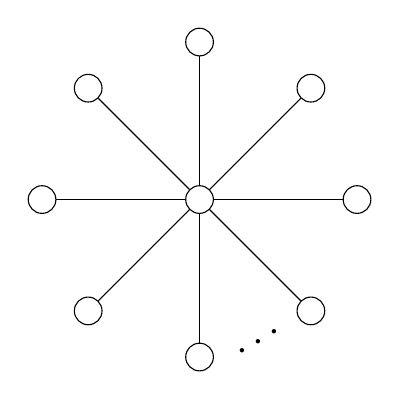
\begin{tikzpicture}
    % Number of outer vertices in the star
    \def\n{8}
    
    % Radius of the star
    \def\r{2cm}
    
    % Rotation angle
    \def\rotationangle{90}
    
    % Draw the central vertex
    \draw (0,0) node[circle, draw, minimum size=10pt, inner sep=1.5pt] (center) {};
    
    % Draw the outer vertices, rotated
    \begin{scope}[rotate=\rotationangle]
      \foreach \i in {1,...,\n} {
        \draw (\i*360/\n:\r) node[circle, draw, minimum size=10pt, inner sep=1.5pt] (\i) {};
      }
    \end{scope}
    
    % Connect the central vertex to every outer vertex
    \foreach \i in {1,...,\n} {
      \draw (center) -- (\i);
    }
    \draw (4) node[shift={(0.75,0.2)}] {\rotatebox{30}{\scalebox{1.5}{$\ldots$}}} (4);
  \end{tikzpicture}
  \]

  Claramente, o raio de uma resposta ótima dessa instância é 1 e inclui o vértice do centro da estrela como um dos centros de cluster.
  Note que se, no algoritmo guloso, o vértice escolhido arbitrariamente for algum dos vértices da ponta dessa estrela o vértice do centro nunca será escolhido, uma vez que ele nunca maximizará a função $c(j,C)$. Assim, serão escolhidos apenas vértices da ponta da estrela e como temos pelo menos $k+1$ delas, sempre existirá um vértice ligado ao centro do seu cluster com uma aresta de custo 2.
% \newpage

\subsection{Método do gargalo}
    Os chamados problemas de gargalo são aqueles definidos em grafos com pesos nas arestas tais que a resposta ótima é o peso de uma aresta.

Para o próximo algoritmo será necessário saber o que é um conjunto independente de vértices.
\begin{definition}
    Seja $G = (V,E)$ um grafo. Um conjunto $S \subseteq V$ é um conjunto \emph{independente} se não existe $e \in E$ que tenha ambos os extremos em $S$.
\end{definition}
Seja $I(G,c,k)$ uma instância do problema dos $k$-centros. Vamos supor que as arestas $E \eqqcolon \{e_1,e_2,\ldots,e_{|E|}\}$ de $G$ estejam dispostas de forma que $c_{e_i} \leq c_{e_{i+1}}$ para todo $i \in [|E|-1]$. Como sabemos que é possível ordenar em tempo polinomial, podemos assumir isso.
Seja $E_i \coloneqq \{e_1,e_2,\ldots,e_i\}$ e $G_i \coloneqq (V,E_i)$. Seja também $i^*$ o menor $i$ tal que $G_i$ tem um $k$-conjunto dominante. Como $G$ é completo, $i^*$ existe. Claramente $c_{e_{i^*}} = \opt(I)$, porém não conseguimos encontrar $i^*$ eficientemente, uma vez que não é possível saber se um grafo tem um $k$-conjunto dominante em tempo polinomial, a menos que $P = \NP$. Vamos usar um conjunto independente maximal para aproximar uma resposta.

\begin{lemma}\label{lemma:2.8}
    Seja $G = (V,E)$ um grafo. Um conjunto independente maximal em $G$ é também um conjunto dominante.
\end{lemma}
\begin{proof}
    Seja $G = (V,E)$ e $S$ um conjunto independente maximal em $G$. Suponha, por absurdo, que $S$ não é um conjunto dominante. Então, existe vértice $u \in V \setminus S$ que não é vizinho de nenhum dos vértices de $S$. Portanto, $S \cup \{u\}$ é também um conjunto independente e $S \subset \{S \cup \{u\}\}$, uma contradição, pois $S$ é maximal.
\end{proof}
Então, se encontrarmos um conjunto independente maximal de tamanho $k$ em $G$ teremos um conjunto dominante de mesmo tamanho. No entanto, não conseguimos garantir que iremos encontrar esse conjunto em $G$ e, por isso, vamos definir e usar o chamado quadrado de $G$.
\begin{definition}
    Seja $G= (V,E)$ um grafo. Denotamos por $G^2 = (V,E^2)$ o \emph{quadrado} de $G$ em que $E^2 = E \cup \{uv: \text{u e v têm vizinhos em comum em $G$}\}$.
\end{definition}
Dada a definição vamos enunciar e provar um lema que nos ajudará no algoritmo.
\begin{lemma}\label{lemma:2.10}
    Seja $G$ um grafo, $G^2$ o seu quadrado e $k$ um inteiro positivo. Se $G$ contém um $k$-conjunto dominante então todo conjunto independente maximal em $G^2$ tem tamanho no máximo~$k$.
\end{lemma}
\begin{proof}
    Vamos mostrar pela contrapositiva.

    Suponha que $G^2$ tem um conjunto independente maximal $S \subseteq V$ tal que $|S| > k$. Seja $D$ um conjunto dominante em $G$. Vamos mostrar que $|D| > k$.

    Por definição, uma aresta entre dois vértices de $S$ em $G^2$ é um caminho de tamanho 2 em $G$. Isso significa que, em $G$, não existe aresta nem vizinho comum entre dois vértices de $S$. Seja $u \in D$. Vamos mostrar que $u$ cobre no máximo um vértice de $S$ em $G$. 
    Se $u \in S$, o único vértice de $S$ coberto por $u$ é ele mesmo, uma vez que não existe aresta entre dois vértices de $S$ em $G$. 
    Se $u \not \in S$, $u$ pode cobrir apenas um vértice de $S$, pois caso cobrisse dois, digamos $v$ e $w$, então u seria um vizinho comum em $G$ de $v$ e $w$ e, portanto, $vw$ seria uma aresta em $G^2$.

    Portanto, $|D| \geq |S| > k$.
\end{proof}
Agora, temos todas as definições e lemas que serão necessários para o algoritmo.
\begin{algorithm}
    \caption{GHS$(G,c,k)$}
    \label{k-center:bottleneck}
    \begin{algorithmic}[1]
        \State $i \leftarrow 0$
        \State $M_0 \leftarrow V$
        \While{$|M_i| > k$}
            \State $i\leftarrow i + 1$
            \State Seja $M_i$ um conjunto independente maximal em $G_i^2$
        \EndWhile
        \State Devolva $M_i$
    \end{algorithmic}
\end{algorithm}

Este algoritmo é de autoria de Gonzalez~\cite{GONZALEZ1985293} e independentemente Hochbaum e Shmoys~\cite{HSBottle}, e, por isso, está sendo creditado com suas iniciais em seu nome. 

\begin{theorem}
    O algoritmo {\sc GHS}$(G,c,k)$ é uma $2$-aproximação do problema dos $k$-centros.
\end{theorem}
\begin{proof}
    Primeiro vamos mostrar que o algoritmo é polinomial. \\
    Como $G_{i^*}$ tem um $k$-conjunto dominante, então o laço vai iterar no máximo $i^* \leq |E|$ vezes, pois pelo Lema~\ref{lemma:2.10} qualquer conjunto independente maximal encontrado em $G_{i^*}^2$ terá tamanho no máximo $k$.
    Também é fácil mostrar que é possível encontrar um conjunto independente maximal em tempo polinomial. Um algoritmo simples começa com um conjunto $A = \{u\}$ sendo $u$ um vértice arbitrário e, a cada iteração, coloca em $A$ um vértice que não é adjacente a nenhum vértice de $A$ até não ser mais possível.
    Além disso, também conseguimos construir o grafo $G_i^2$ em tempo polinomial. Começaremos $E_i^2$ como uma cópia de $E_i$ e, para cada tripla de vértice $(u,v,w)$ caso já não exista uma aresta $uw \in E_i$, vamos inseri-la em $E_i^2$ se $v$ for um vizinho comum de $u$ e $w$ em $E_i$. Como temos no máximo $|V|^3$ triplas de vértices e todas as operações que serão feitas tomam tempo polinomial, então podemos construir $G_i^2$ em tempo polinomial.

    Agora, vamos mostrar que o algoritmo é uma $2$-aproximação.

    Para um grafo $H$ com peso nas arestas, definimos max$(H)$ como o maior peso de uma aresta. Seja $i'$ o valor de $i$ ao final do algoritmo e $M_{i'}$ a solução devolvida por ele. Como $M_{i'}$ é um conjunto independente maximal de tamanho no máximo $k$, então pelo Lema~\ref{lemma:2.8} ele é um $k$-conjunto dominante e como o grafo induzido $G_{i'}[M_{i'}]$ é um subgrafo de $G_{i'}^2$ então max$(G_{i'}[M_{i'}]) \leq \text{max}(G_{i'}^2) $. Pela desigualdade triangular, é fácil notar que max$(G_{i'}^2) \leq 2$  max$(G_{i'})$. Assim, max$(G_{i'}[M_{i'}]) \leq $ max$(G_{i'}^2) \leq 2$ max$(G_{i'}) \leq 2$ max$(G_{i^*})= 2 \opt(I)$. 
\end{proof}


% \newpage

\section{Localização de instalações}
    Antes de falarmos sobre algoritmos de aproximação para o problema da localização de instalações, vamos mostrar que, assumindo $P\neq\NP$, não existe algoritmo polinomial que resolva nosso problema, ou seja, vamos mostrar que nosso problema é $\NP$-difícil. Para isso, vamos definir o problema da cobertura por vértices.



\begin{problem}(Cobertura por vértices)
    Dado um grafo $G$ e um inteiro $k$, decidir se $G$ tem uma cobertura por vértices de tamanho $k$.
\end{problem}
Esse problema é $\NP$-completo, sendo um dos famosos $21$ problemas do Karp~\cite{Karp1972}. Disso deriva-se o seguinte.

\begin{theorem}
    O problema de localização de instalações é $\NP$-difícil.
\end{theorem}

\begin{proof}
    Suponha que exista um algoritmo $A$ que resolva o problema de localização de instalações em tempo polinomial.

    Seja $I(G,k)$ uma instância do problema da cobertura por vértices. Tome $F \coloneqq V(G)$ e $D \coloneqq E(G)$. Considere também $f_i = 1$ para todo $i \in V$ e $c_{ij} = 0$ se $i \in V(G)$ é extremo de $j \in E(G)$ e 2 caso contrário. Assim, construímos uma instância $I'(F,D,c,f)$ do problema de localização de instalações a partir de uma instância do problema da cobertura por vértices. 

    Note que a resposta ótima de $I'$ será a menor quantidade de instalações que precisamos abrir até que todos os clientes possam ser associados a instalações em que o seu custo de associação é 0. Se um cliente(aresta) está associado a uma instalação(vértice) cujo custo de associação é 2, podemos diminuir o custo total abrindo uma instalação em que o custo de sua associação é 0, uma vez que abrir a instalação custaria 1 e diminuiríamos o custo de associação do cliente de 2 para 0. Sabemos que essa instalação existe, pois para cada cliente(aresta) existem duas instalações com custo de associação 0(seus vértices extremos).
    Assim, é fácil notar que essa quantidade de instalações é o tamanho mínimo de uma cobertura por vértices em $G$. Portanto, se o custo total da solução do algoritmo $A$ aplicado à instância $I'$ é menor ou igual a $k$, então a resposta para $I$ é sim. Caso contrário, a resposta é não.

    Desse modo, resolvemos o problema da cobertura por vértices em tempo polinomial, o que, assumindo $P\neq\NP$, é um absurdo.
\end{proof}

\subsection{Algoritmos baseados em programação linear}
    \label{facility:PL}
    Nessa seção vamos mostrar algoritmos para o problema de localização de instalações que utilizam métodos baseados em programação linear.

Vamos modelar o problema de localização de instalações como um programa linear inteiro. Vamos relaxar esse programa e encontrar o seu dual.

Para uma instância $(F,D,c,f)$ do problema de localização de instalações, o programa inteiro terá dois tipos de variáveis. Uma variável $y_i$ para cada $i \in F$ que terá valor 1 se a instalação $i$ foi aberta e 0, caso contrário, e uma variável $x_{ij}$, para cada $i \in F$ e $j \in D$, que terá valor 1 se o cliente $j$ estiver associado a instalação $i$ e 0, caso contrário. 

Assim, uma instância $(F,D,c,f)$ do problema de localização de instalações pode ser modelada como o seguinte programa linear inteiro:
\begin{align}
 \text{Minimizar} \quad & \sum_{i \in F}f_iy_i + \sum_{i\in F,j\in D}c_{ij}x_{ij} \nonumber \\
 \text{sujeito a} \quad & \sum_{i\in F} x_{ij}\geq1, \quad \forall j \in D \label{eq:inst}\\
 &x_{ij} \leq y_i,\quad \quad \; \; \forall i\in F,j\in D \label{eq:fac} \\
 &x_{ij} \in \{0,1\} ,\quad \forall i\in F,j\in D \label{fl:x}\\
 &y_i \in \{0,1\}, \quad \; \,\forall i\in F \label{fl:y}.
\end{align}
A restrição~\eqref{eq:inst} garante que todo cliente esteja associado a alguma instalação, a restrição~\eqref{eq:fac} garante que todo cliente esteja associado apenas a instalações abertas.

Para a relaxação desse programa permitiremos que as variáveis em $x$ e em $y$ adotem quaisquer valores não negativos. Portanto, a relaxação do programa inteiro do problema de localização de instalações resulta no seguinte programa.

    \begin{align}
        \text{Minimizar} \quad & \sum_{i \in F}f_iy_i + \sum_{i\in F,j\in D}c_{ij}x_{ij} \tag{PL} \label{P1}\\
        \text{sujeito a} \quad & \sum_{i\in F} x_{ij}\geq1,  &&\forall j \in D \tag{P2} \label{P2}\\
        &y_i - x_{ij} \geq 0, &&\forall i\in F,j\in D \tag{P3} \label{P3}\\
        &x_{ij} \geq 0, &&\forall i\in F,j\in D\tag{P4}\label{P4}\\
        &y_i \geq 0, &&\forall i\in F. \tag{P5} \label{P5}
       \end{align}

       O dual do programa linear acima consiste no seguinte programa.
    \label{D}
    \begin{align}
        \text{Maximizar} \quad & \sum_{j \in D} v_{j}  \tag{PD} \label{D1}\\
        \text{sujeito a} \quad & \sum_{j\in D} w_{ij}\leq f_i, &&\forall i \in F \tag{D2} \label{D2}\\
        &v_{j} - w_{ij}\leq c_{ij},  &&\forall i\in F,j\in D \tag{D3} \label{D3}\\
        &w_{ij} \geq 0 , &&\forall i\in F,j\in D\tag{D4} \label{D4}\\
        &v_j \geq 0, &&\forall j\in D \tag{D5} \label{D5}.
       \end{align}

Sabemos que cada variável de um destes programas está associada a uma restrição do outro programa. 
Especificamente, a variável $x_{ij}$ está associada à desigualdade~\eqref{D3}, a variável $y_i$ está associado à desigualdade~\eqref{D2}, a variável $w_{ij}$ está associada à desigualdade~\eqref{P3} e a variável $v_j$ está associado a desigualdade~\eqref{P2}.

Note que toda solução viável do programa linear inteiro é solução viável do programa linear relaxado. Desse modo, a resposta ótima do programa linear relaxado tem valor objetivo no máximo o valor objetivo da resposta ótima do programa linear inteiro.

Vamos aqui interpretar o programa dual. Chamaremos as variáveis $v$ de orçamento e as variáveis $w$ de contribuição. Dizemos que um cliente $j$ \emph{contribui} para uma instalação $i$ se $w_{ij} > 0$. Uma instalação recebe contribuições dos clientes para pagar pela sua abertura. Uma vez que as contribuições são suficientes para a sua abertura, a instalação não precisa receber mais contribuições. Isso está explicito na restrição~\eqref{D2}.

O orçamento de um cliente é no máximo o custo de sua associação a uma instalação e sua contribuição para a abertura dela. Isso está explicito na restrição~\eqref{D3}.

Para entender como as variáveis primais e duais se relacionam, vamos analisar as condições de folgas complementares. Vamos supor a existência de uma solução ótima inteira $(x^*,y^*)$ para o primal e seja $(v^*,w^*)$ uma solução ótima para o dual. Em uma solução inteira do primal, as variáveis $x$ e $y$ satisfazem as restrições do programa inteiro. Como ambas são soluções ótimas, valem as folgas complementares. A partir dos pares variável-restrição correspondentes já vistos, as condições de folgas complementares estabelecem que
\begin{enumerate}[(i)]
    \item para todo $i \in F$ e $j \in D$, se $x^*_{ij} > 0$ então $v^*_j - w^*_{ij} = c_{ij}$\label{fg:i};
    \item para todo $ i \in F$, se $y^*_i > 0$ então $\sum_{j \in D} w^*_{ij} = f_i$\label{fg:ii};
    \item para todo $i \in F$ e $ j \in D$, se $w^*_{ij}>0$ então $ y_i = x_{ij}$\label{fg:iii};
    \item para todo $j \in D$ se $v^*_j > 0$  então $\sum_{i \in F}x^*_{ij} = 1$\label{fg:iv}.
\end{enumerate}
Pela condição~\eqref{fg:i}, se um cliente $j$ está associado a uma instalação $i$ então o orçamento do cliente $j$ é exatamente o custo dele se associar a $i$ mais a sua contribuição para a abertura de~$i$. Então podemos interpretar $v_j$ como o valor que o cliente paga para a instalação a qual ele estará associado. 
Pela condição~\eqref{fg:ii}, cada instalação aberta precisa ter contribuições suficientes para pagar pela sua abertura. Pela condição~\eqref{fg:iii}, temos que um cliente que contribui para uma instalação aberta está associado a ela. Juntando as condições~\eqref{fg:ii} e \eqref{fg:iii}, temos que as contribuições recebidas pelas instalações abertas são vindas apenas de clientes associados a elas e são suficientes para pagar pela sua abertura. 
Pela condição~\eqref{fg:iv}, um cliente que tem orçamento não nulo está associado a exatamente uma instalação.

\subsubsection{Método primal-dual}
    Nessa seção vamos apresentar o algoritmo primal-dual para o problema de localização de instalações. Esse algoritmo foi estudado na seção 7.6 do livro WS2011 e foi desenvolvido pelo Jain e pelo Vazirani~\cite{JV}.

Vamos assumir que a função custo satisfaz a desigualdade triangular. Como a função custo só está definida de um cliente para uma instalação, então a desigualdade triangular terá uma cara diferente. Para clientes $j,l$ e  instalações $i,k$, vale que
\[c_{ij} \leq c_{il} + c_{kl} + c_{kj}.\]

Chamamos uma solução $(v,w)$ para o programa dual de \emph{maximal} se não existe solução viável $(v',w')$ tal que:
\begin{enumerate}[(i)]
    \item $v_j \leq v'_j$ para todo cliente $j$;
    \item $w_{ij} \leq w'_{ij}$ para todo cliente $j$ e instalação $i$;
    \item $v_j < v'_j$ para algum cliente $j$;
\end{enumerate}
ou seja, não conseguimos encontrar uma solução viável com valor objetivo maior apenas aumentando os valores das variáveis.

Vamos utilizar a seguinte definição ao longo da explicação do método.
\begin{definition}
    Seja $(v,w)$ uma solução viável do dual. Denotamos por $N(j) = \{i \in F:v_j \geq c_{ij}\}$ a \emph{vizinhança} de um cliente $j$ e $N(i) = \{j \in D:v_j \geq c_{ij}\}$ a \emph{vizinhança} de uma instalação $i$.
\end{definition}

\begin{theorem}
    Seja $(\overline v, \overline w)$ solução maximal para o programa dual e $T \coloneqq \{i \in F: \sum_{j \in D} \overline{w}_{ij} = f_i\}$. Então, todo cliente está na vizinhança de uma instalação em $T$.      
\end{theorem}
\begin{proof}
    Vamos provar por absurdo. Suponha a existência de um cliente $j$ que não está na vizinhança de nenhuma instalação em $T$. Claramente, as desigualdades~\eqref{D3} não são justas para $j$ e nenhuma instalação em $T$. Assim, conseguimos aumentar $\overline{w}_{ij}$ para uma instalação $i$ qualquer que não esteja em $T$, aumentando simultaneamente o $\overline{v}_j$ sem infringir nenhuma das restrições do dual. Com isso, apenas aumentando os valores das variáveis, conseguimos encontrar uma solução viável do dual com valor objetivo maior e isso contradiz o fato da solução $(\overline{v},\overline{w})$ ser maximal. 
\end{proof}

Como cada cliente está na vizinhança de uma instalação que pertence a $T$, abrir todas as instalações em $T$ seria suficiente, mas um cliente poderia contribuir para mais que uma instalação de $T$. Assim, possivelmente estaríamos contando o orçamento de um cliente na contribuição para a abertura de mais de uma instalação, o que interferiria na comparação do custo da solução com o valor ótimo.
Para evitar este problema, podemos escolher um conjunto $T' \subseteq T$ tal que cada cliente esteja na vizinhança de no máximo uma instalação de $T'$ e vamos garantir que um cliente que não esteja na vizinhança de nenhuma instalação de $T'$ esteja próximo a alguma delas.

Nosso algoritmo contará com as seguintes invariantes.
\begin{itemize}
    \item $(v,w)$ é uma solução viável do programa dual.
    \item $T$ são as instalações que têm contribuições suficientes para serem abertas.
    \item $S$ é o conjunto de clientes que não têm nenhum vizinho em $T$.
\end{itemize}
\begin{algorithm}[tbh]
    \caption{\sc PrimalDual-JV(${F,D,c,f}$)}
    \label{fl:primaldual}
    \begin{algorithmic}[1]
        \State $v_j \gets 0$ para todo $j \in D$
        \State $w_{ij} \gets 0$ para todo $i \in F$ e $j \in D$
        \State $S \gets D$
        \State $T \gets \emptyset$
        \While{$S \neq \emptyset$}
        \State $\theta_1 \gets \min\{c_{ij}-v_j : j \in D \text{ e } i \not\in N(j)\}$ \label{theta1}
        \State $\theta_2 \gets \min\{(f_i - \sum_{j \in N(i)}w_{ij})/|N(i)| : i \in F \text{ tal que } N(i) \neq \emptyset \} \label{theta2}$
        \State $\theta \gets \min\{\theta_1,\theta_2\} \label{theta}$
        \State $v_j \gets v_j + \theta$ para todo $j \in D$
        \State $w_{ij} \gets w_{ij} + \theta$ para todo $j \in D$ e $i \in N(j)$ 
        \If{$v_j = c_{hj}$ para algum $j \in S$ e $h \in T$}
        \State $S \gets S \setminus \{j\}$
        \EndIf
        \If{$\sum_{j \in N(i)} w_{ij} = f_i$ para algum $i \not \in T$}
        \State $T \gets T \cup \{i\}$
        \State $S \gets S\setminus N(i)$
        \EndIf
        \EndWhile
        \State $T' \gets \emptyset$
        \While{$T \neq \emptyset$}
        \State Escolha $i \in T$
        \State $T' \gets T' \cup \{i\}$
        \State $T \gets T \setminus \{h \in T : \text{existe $k \in D$ com $w_{ik}> 0 $ e $w_{hk} > 0$} \}$
        \EndWhile
        \State \Return $T'$
    \end{algorithmic}
\end{algorithm}

No algoritmo {\sc PrimalDual-JV}, claramente as coordenadas das variáveis $v$ e $w$ crescerão de maneira uniforme, pois em cada iteração o mesmo valor $\theta$ será somado a elas. Precisamos então garantir que a nossa solução seja sempre viável. Pela escolha de $\theta_1$ na linha~\ref{theta1} do algoritmo, garantimos que a desigualdade~\eqref{D3} não seja violada para $i$ e $j$ em que $i$ é uma instalação que não está na vizinhança do cliente $j$. Quando a instalação $i$ está na vizinhança de $j$, aumentamos $v_j$ e $w_{ij}$ do mesmo valor $\theta$ e isso nunca violará a desigualdade~\eqref{D3}. 
Pela escolha de $\theta_2$ na linha~\ref{theta2}, garantimos que a desigualdade~\eqref{D2} não seja violada para nenhuma instalação. 
Assim, $(v,w)$ é uma solução viável para o problema dual durante todo o algoritmo.
Para cada cliente $j$ e cada instalação $i$, primeiro aumentaremos apenas as variáveis $v_j$ até que $j$ esteja na vizinhança de $i$. Note que nesse momento a desigualdade~\eqref{D3} se torna justa, pois ainda não aumentamos a variável $w_{ij}$. Uma vez que isso acontece, aumentamos uniformemente $v_j$ e $w_{ij}$, assim a desigualdade~\eqref{D3} continuará justa. Desse modo, para $j \in D$ e $i \in N(j)$, vale que 
\begin{equation}\label{Djusta:*}  
w_{ij} = v_j - c_{ij}.
\end{equation}
Note também que ao final do algoritmo $(v,w)$ é uma solução maximal para o problema dual. Isso acontece pois para todo cliente $j$ existe uma instalação $i$ tal que a desigualdade~\eqref{D3} é justa para $i$ e $j$ e, além disso, a desigualdade~\eqref{D2} é justa para $i$. Desse modo, não conseguimos encontrar uma solução viável com valor objetivo maior apenas aumentando as variáveis, pois $w_{ij}$ não pode ser aumentado e é ele quem está impedindo o aumento de $v_j$.

Para provar a razão de aproximação vamos precisar primeiro de um lema.
\begin{lemma}
    \label{lemma:3.9}
    Seja $T'$ a solução devolvida e $(v,w)$ solução do dual produzida pelo Algoritmo {\sc PrimalDual-JV }. Se $j \in D$ não está na vizinhança de nenhuma instalação de $T'$, então existe uma instalação $i \in T'$ tal que $c_{ij} \leq 3v_j$.
\end{lemma}
\begin{proof}
    Seja $h \in T$ a instalação responsável pela remoção de $j$ de $S$, conforme a linha 12 ou 16 do algoritmo. Claramente, $j$ pertence a vizinhança de $h$. Sabemos que $h$ não pertence a $T'$ uma vez que, por hipótese, $j$ não tem vizinhos em $T'$. Como $h$ foi retirada de $T$, conforme a linha 21 do algoritmo, existe $i \in T'$ e $k \in D$ tal que $k$ contribui para $i$ e para $h$. Pela desigualdade triangular,
    \[c_{ij} \leq c_{hj} + c_{hk} + c_{ik}\]
    como $j \in N(h)$ e $k \in N(h) \cap N(i)$ vale que $c_{hj} \leq v_j$ e $c_{hk} + c_{ik} \leq 2v_k$. Como $k$ contribui para $h$, então $k$ já estava na vizinhança de $h$ no momento que $h$ foi retirado de $T$. Assim, $k$ saiu de $S$ no mesmo momento ou anterior a $h$ sair de $T$. Como $h$ foi responsável pela retirada de $j$ de $S$, então $j$ não foi retirado de $S$ antes de $k$. Como as variáveis crescem de maneira uniforme, então $v_k \leq v_j$. 
    Portanto, $c_{ij}\leq 3v_j$. 
\end{proof}

Agora, podemos mostrar o teorema abaixo.
\begin{theorem}
    O algoritmo {\sc PrimalDual-JV} é uma $3$-aproximação para o problema da localização de instalações.
\end{theorem}
\begin{proof}
    Claramente o algoritmo roda em tempo polinomial. 

    Para cada cliente que contribui para uma instalação de $T'$, vamos associá-lo a essa instalação. Como cada cliente contribui para no máximo uma instalação de $T'$, então essa associação é única. Para clientes que estão na vizinhança de instalações de $T'$, mas não contribuem para nenhuma delas, vamos associá-los a qualquer instalação de $T'$ na sua vizinhança.
    Seja $A(i) \subseteq N(i)$ os clientes vizinhos associados a instalação $i \in T'$. Então o custo de abertura das facilidades em $T'$ mais o custo de associar os clientes vizinhos é
    \[\sum_{i \in T'} (f_i + \sum_{j \in A(i)} c_{ij}) = \sum_{i \in T'} \sum_{j \in A(i)} (w_{ij} + c_{ij}) = \sum_{i \in T'} \sum_{j \in A(i)} v_j\]
    em que a primeira igualdade vale pela definição de $T$ e a segunda igualdade vale por~\eqref{Djusta:*} e também pois $w_{ij} > 0$ implica $j \in A(i)$. Claramente o somatório não repete clientes, uma vez que cada cliente está associado a apenas uma instalação.

    Para um cliente $j$ que não está na vizinhança de nenhuma instalação de $T'$, podemos utilizar o Lema~\ref{lemma:3.9}. Então existe uma instalação de $i \in T'$ tal que $c_{ij} \leq 3v_j$. Vamos associar $j$ a $i$. Seja $Z$ o conjunto de clientes que não têm vizinhos em $T'$. Temos
    \[\sum_{j \in Z}c_{\sigma(j)j} \leq 3\sum_{j \in Z}v_j.\]
    Juntando os limitantes encontrados para os clientes que têm vizinhos em $T'$ e os que não têm, encontramos
    \[\sum_{i \in T'} (f_i + \sum_{j \in A(i)} c_{ij}) + \sum_{j \in Z} c_{\sigma(j)j}\leq \sum_{i \in T'} \sum_{j \in A(i)} v_j + 3 \sum_{j \in Z} v_j \leq 3 \sum_{j \in D} v_j\leq 3\,\opt(I)\]
    em que a última desigualdade vale pela dualidade fraca.
\end{proof}

\subsubsection{Arredondamento do programa linear}
    Nessa seção vamos apresentar o algoritmo que faz arredondamento determinístico de uma solução relaxada do programa inteiro que modela o problema localização de instalações. Esse algoritmo foi estudado na seção 4.5 do livro WS2011 e foi desenvolvido pelo Chudak e Shmoys~\cite{Chudak2003}.


Vamos então definir algumas coisas que serão necessárias no nosso algoritmo.
\begin{definition}
    Seja $(x^*,y^*)$ uma solução do programa linear. Dizemos que uma instalação $i$ está na \emph{vizinhança} de um cliente $j$ se $x^*_{ij} > 0$. Seja $N(j) = \{ i \in F : x^*_{ij} > 0\}$.
\end{definition}
Dada essa definição, vamos enunciar um lema que irá nos ajudar a provar uma cota superior para o custo de associação da solução aproximada escolhida pelo algoritmo.
\begin{lemma}\label{lemma:3.5}
    Sejam $(x^*,y^*)$ e $(v^*,w^*)$ soluções do programa linear e do seu dual, respectivamente, e $j$ um cliente qualquer. Para todo $i \in N(j)$, $c_{ij} \leq v^*_j$.
\end{lemma}
\begin{proof}
    Como $i \in N(j)$, então $x^*_{ij}>0$. Assim, pelas folgas complementares, a desigualdade do dual correspondente a~\eqref{P4} vale por igualdade, então $v^*_j - w^*_{ij} = c_{ij}$. Como $w^*_{ij} \geq 0$, $c_{ij} \leq v^*_j$. 
\end{proof}
Com esse lema, sabemos que se em um conjunto $S \subseteq F$ de instalações abertas, para todo cliente $j \in D$, existe uma instalação aberta $i$ em $N(j)$, então $c_{ij}\leq v_j^*$ e o custo total de associação seria no máximo $\sum_{j\in D}v_j^* \leq \opt(I)$. Entretanto, não é garantido uma cota superior para o custo de abertura de $S$. Vamos descobrir como encontrar um $S$ com um bom custo de abertura e um bom custo de associação. Seja $j_k$ um cliente qualquer. Se abrirmos a instalação $i_k$ mais barata de $N(j_k)$ conseguimos limitar o custo de sua abertura por
\[\tag{*} \label{relx_fl:*}
    f_{i_k} = f_{i_k} \sum_{i \in N(j_k)}x^*_{ij_k} = \sum_{i \in N(j_k)}f_{i_k}x^*_{ij_k} \leq \sum_{i \in N(j_k)}f_{i}y^*_{i},
\]
onde a primeira igualdade vale por \eqref{P3} e pela definição de $N(j_k)$ e a desigualdade vale por termos escolhido $i_k$ como a instalação mais barata de $N(j_k)$.

Essa informação será importante para a prova da razão de aproximação do nosso algoritmo. Agora, faremos uma última definição necessária para o nosso algoritmo.

\begin{definition}
    Seja $j\in D$ um cliente. Seja $N^2(j)$ o conjunto dos clientes $i \in D$ tais que $N(i) \cap N(j) \neq \emptyset$.
\end{definition}
Agora, vamos definir o algoritmo. Nele, $S$ será o conjunto das instalações a serem abertas e $\sigma : D \rightarrow F $ a função que associa cada cliente a uma instalação aberta. Ambos serão montados durante o algoritmo.
\begin{algorithm}
    \caption{\sc ArredDet-CS($F,D,c,f$)}
    \label{fl:plrounding}
    \begin{algorithmic}[1]
        \State Sejam $(x^*,y^*)$ e $(v^*,y^*)$ soluções ótimas para o primal e o dual da relaxação do programa inteiro de $I(F,D,c,f)$.
        \State $S \gets \emptyset$
        \State $C_0 \gets D$ 
        \State $k \gets 0$
        \While{$C_k \neq \emptyset$}
        \State Escolha $j_k \in C_k$ que minimize $v_j^*$
        \State Escolha $i_k \in N(j_k)$ que minimize $f_{i}$
        \State $S \gets S \cup \{i_k\}$
        \State Associe a instalação $i_k$ a cada cliente em $N^2(j_k) \cap C_k$
        \State $C_{k+1} \gets C_k \setminus N^2(j_k)$
        \State $k \gets k+1$
        \EndWhile
        \State \Return $S$
    \end{algorithmic}
\end{algorithm}

\begin{theorem}
    O algoritmo {\sc ArredDet-CS} é uma $4$-aproximação para o problema da localização de instalações.
\end{theorem}
\begin{proof}
    Primeiro, vamos mostrar que o algoritmo é polinomial. Sabemos que é possível encontrar uma solução para o problema linear e o seu dual em tempo polinomial utilizando o método dos elipsoides~\cite{Kha79}. Sabemos que o laço da linha 5 irá executar no máximo $|D|$ iterações, uma vez que sempre retiramos pelo menos um elemento de $C$. Além disso, as linhas $6-12$ são claramente polinomiais.

    Agora, vamos mostrar que o algoritmo é uma $4$-aproximação.
    Perceba que, para $k_1$ e $k_2$ com $k_1 < k_2$, $N(j_{k_1})\cap N(j_{k_2}) = \emptyset$, caso contrário $j_{k_2} \in N^2(j_{k_1})$ e não estaria em~$C_{k_2}$.
    Seja $F' \subseteq F$, tal que $F' = \bigcup_k N(j_k)$.
    Por \eqref{relx_fl:*}, vale que $f_{i_k} \leq \sum_{i \in N(j_k)}f_{i_k}y^*_{i}$. Então se somarmos para todo $k$, temos
    \[ \sum_kf_{i_k} \leq \sum_k \sum_{i \in N(j_k)}f_{i}y^*_{i} = \sum_{i \in F'}f_{i}y^*_{i} \leq \sum_{i \in F}f_{i}y^*_{i} \leq \opt(I).\]

    Agora, vamos fixar uma iteração $k$ e sejam $i = i_k$ e $j = j_k$. Pelo Lema~\ref{lemma:3.5}, sabemos que $c_{ij} \leq v^*_j$. Seja $\ell \in N^2(j) \cap C_k$ diferente de $j$ e $h \in N(\ell) \cap N(j)$. Pela desigualdade triangular e como $j$ minimiza $v^*_j$ em $C_k$, temos
    \[ c_{i\ell} \leq c_{ij} + c_{hj} + c_{h\ell} \leq v_j^* + v_j^* + v_{\ell}^* \leq 3 v_{\ell}^*.
        \]
    Então, temos que
    \begin{subequations}
        \begin{align*}
        \sum_{k} {\big (}c_{i_kj_k} + \sum_{j \in N^2(j_k)\cap C_k} c_{i_kj} {\big )} &= \sum_{k} c_{i_kj_k} + \sum_{k}\sum_{j \in N^2(j_k)\cap C_k} c_{i_kj}\\
        &\leq \sum_k v^*_{j_k} + 3\sum_{k}\sum_{j \in N^2(j_k)\cap C_k} v^*_j\\
        &\leq 3 \sum_{j \in D}v^*_j \leq 3\opt(I)           
        \end{align*}
    \end{subequations}
    em que a penúltima desigualdade vale pois o algoritmo só para quando $C_k$ é vazio.

    Assim, temos que o custo de abertura das instalações é no máximo $\opt(I)$ e o custo de associação é no máximo $3\opt(I)$. Portanto, o custo total da solução $S$ é no máximo $4~\opt(I)$.
\end{proof}

\subsubsection{Arredondamento probabilístico}
    Nessa seção vamos apresentar o algoritmo que faz arredondamento probabilístico de uma solução relaxada do programa inteiro que modela o problema localização de instalações. Esse algoritmo foi estudado na seção 5.8 do livro WS2011 e foi desenvolvido pelo Chudak e Shmoys~\cite{Chudak2003}.

Vamos rever definições já vistas anteriormente. 
Seja $I(F,D,c,f)$ uma instância do problema de localização de instalações e $(x^*,y^*)$ uma solução da relaxação do programa inteiro referente a $I$. 
Denote os vizinhos de um cliente $j$ como $N(j) \coloneqq\{i \in F : x^*_{ij} > 0\}$. 
Denote também os vizinhos dos vizinhos de um cliente $j$ como $N^2(j) \coloneqq \{ k \in D : \text{ existe algum } i \in N(j) \text{ tal que } x^*_{ik} > 0\}$.
Além disso, defina $C^*_j \coloneqq \sum_{i \in F} c_{ij}x^*_{ij}$ .

\begin{algorithm}[tbh]
\caption{\sc ArredProb-CS($F,D,c,f$)}
\begin{algorithmic}[1]
        \State Sejam $(x^*,y^*)$ e $(v^*,y^*)$ soluções ótimas para o primal e o dual da relaxação do programa inteiro de $I(F,D,c,f)$.
        \State $S \gets \emptyset$
        \State $C_0 \gets D$
        \State $k \gets 0$
        \While{$C_k \neq \emptyset$}
        \State Escolha $j_k \in C_k$ que minimize $v^*_j + C^*_j$
        \State Escolha $i_k \in N(j_k)$ de acordo com a distribuição de probabilidade $x^*_{ij_k}$
        \State $S \gets S \cup \{i_k\}$
        \State Associe a instalação $i_k$ a cada cliente em $N^2(j_k) \cap C_k$
        \State $C_{k+1} \gets C_k \setminus N^2(j_k)$
        \State $k \gets k +1$
        \EndWhile
        \State \Return $S$
\end{algorithmic}
\end{algorithm}

\begin{theorem} O algoritmo {\sc ArredProb-CS} é uma 3-aproximação para o problema da localização de instalações.
\end{theorem}

\begin{proof}
É evidente que o algoritmo toma tempo polinomial.

Note que, para um mesmo par de soluções ótimas do primal e do dual, a escolha de $j_k$ para uma iteração $k$ qualquer é determinística e, portanto, $N^2(j_k) \cap C_k$ é sempre igual para uma iteração $k$. Assim, o valor esperado da nossa solução é a soma, para cada $k$, do valor esperado de $f_{i_k}$ mais o custo esperado de transporte para cada cliente associado a $i_k$. 

Seja $k$ uma iteração qualquer. Seja $X_k$ uma variável aleatória que represente o custo de abertura da instalação escolhida na iteração $k$, então
\[ \mathbb{E}[X_k] = \sum_{i \in j_k} f_i x^*_{ij_k} \leq \sum_{i \in N(j_k)} f_i y^*_i\]
onde a desigualdade vale pela restrição~\ref{P3}. Seja $Y_k^j$ a variável aleatória que represente o custo de transporte do cliente $j \in N^2(j_k) \cap C_k$. Assim, o valor esperado para o custo de abertura de $j_k$ é 
\[\mathbb{E}[Y_k^{j_k}] = \sum_{i \in N(j)} c_{ij_k} x^*_{ij_k} = C^*_{j_k}. \]
Seja $\ell$ um cliente em $N^2(j_k) \cap C_k$ diferente de $j_k$ e $h \in N(j_k)$ tal que $x^*_{h\ell} > 0$, note que $h$ existe pela definição de $N^2(j_k)$. Pela desigualdade triangular vale que $c_{i\ell} \leq c_{ij_k} + c_{hj_k} + c_{hj}$ e, portanto,
\begin{subequations} 
        \begin{align*}
        \mathbb{E}[Y_k^\ell] = \sum_{i \in N(j_k)} c_{i\ell}x^*_{ij_k} &\leq \sum_{i \in N(j_k)} (c_{ij_j} + c_{hj} + c_{h\ell})x^*_{ij_k} = c_{hj} + c_{h\ell} + C^*_{j_k}\\
        &\leq v^*_\ell + v^*_{j_k} + C^*_{j_k} \leq 2v^*_{\ell} + C^*_\ell 
        \end{align*}
\end{subequations}
onde a segunda desigualdade vale pelo Lema~\ref{lemma:3.5} e a terceira vale pela escolha de $j_k$.

Então fica evidente que o valor esperado da nossa solução é 
\begin{subequations}
        \begin{align*}
                \sum_k {\big (}\mathbb{E}[X_k] + \sum_{j \in N^2(j_k)\cap C_k}\mathbb{E}[Y_k^j] {\big )} &\leq \sum_k {\big (} \sum_{i \in N(j_k)}f_iy^*_i + \sum_{j \in N^2(j_k) \cap C_k} (2v^*_j + C^*_j) {\big )}  \\
                & = \sum_k \sum_{i \in N(j_k)}f_iy^*_i + \sum_k \sum_{j \in N^2(j_k)\cap C_k}(2v^*_j + C^*_j)\\
                &\leq\sum_{i \in F} f_iy^*_i + \sum_{j \in D }(2v^*_j + C^*_j)\\
                &= \sum_{i \in F} f_iy^*_i + \sum_{i \in F, j \in D} c_{ij}x^*_{ij} + 2\sum_{j \in D}v_j \\
                &\leq 3 \opt(I)
        \end{align*}
\end{subequations}
onde a segunda igualdade vale pois para $k_1 < k_2$, vale que $N(j_{k_1}) \cap N(j_{k_2}) = \emptyset$, caso contrário $j_{k_2}$ estaria em $N^2(j_{k_1})$ e, portanto, não estaria em $C_{k_2}$.
\end{proof}


% \newpage

\subsection{Busca local}
    Nessa seção falaremos sobre o algoritmo de busca local para o problema de localização de instalações métrico. Esse algoritmo foi estudado na Seção 9.1 do livro WS2011 e foi proposto primeiramente por Kuen e Hamburger~\cite{KH}. Charikar e Guha~\cite{Charikar&Guha'05} provaram a razão de aproximação igual a 3 e introduziram a ideia de reescala, porém a análise a ser apresentada foi feita por Gupta e Tangwongsan~\cite{DBLP:journals/corr/abs-0809-2554}.

Numa instância $(F,D,c,f)$ do problema de localização de instalações, o custo de transporte está definido apenas para um cliente e uma instalação.
Definimos o custo de transporte entre duas instalações como o menor custo de transporte entre essas duas instalações passando por um cliente qualquer. Igualmente, definimos o custo de transporte entre dois clientes como o menor custo de transporte entre esses dois clientes passando por uma instalação qualquer. Então a desigualdade triangular valerá da seguinte forma: para todo $i,j,\ell \in F \cup D$, 
\[ c_{ij} \leq c_{i\ell} + c_{\ell j}.\]

Um algoritmo de busca local começa com uma solução viável para o problema e checa se alguma alteração local melhora o custo da solução atual. Caso essa melhora ocorra, essa alteração é feita. Esse processo se repete até que não exista alteração local que melhore o custo da solução corrente. A solução resultante é chamada de \emph{localmente ótima}. O tempo de execução de uma implementação dessa ideia e a qualidade da solução obtida dependem da definição adotada de alteração local. Quanto mais abrangente essa definição, melhor a solução, porém em geral mais lento será o algoritmo. Quanto mais restrita a definição, mais rápido o algoritmo, porém pior em geral a qualidade da solução final. Usualmente adotam-se restrições mínimas que garantam a polinomialidade do algoritmo.

O algoritmo que descreveremos contará com três operações: abrir instalações fechadas, fechar instalações abertas ou trocar uma instalação aberta por uma fechada. A solução inicial terá todas as instalações abertas. Para garantir a polinomialidade, uma operação só será feita se diminuir o custo da solução atual em uma razão de $1-\delta$, para um $\delta>0$. Como essa solução não é necessariamente localmente ótima, iremos chamá-la de solução \emph{quase localmente ótima}. Ao final, mostraremos que, dado um $\eps > 0$, o algoritmo é uma $3(1 + \epsilon)$-aproximação para o problema de localização de instalações métrico, onde o $\delta$ será escolhido em função do $\epsilon$ e o consumo de tempo do algoritmo será afetado pelo valor de $\delta$.

\begin{algorithm}
    \caption{\sc BuscaLocal$_\eps$-KHCGGT$(F,D,c,f)$}
    \begin{algorithmic}[1]
        \State $\delta \gets \frac{\eps}{(1+\eps)2|F|}$
        \State $ S' \gets F $ 
        \Repeat
        \State $S\gets S'$
        \If{existe $i \in S$ tal que custo$(S\setminus \{i\} ) \leq (1-\delta) $ custo$(S)$}
        \State $S' \gets S \setminus \{i\}$
        \EndIf
        \If{existe $i' \in F\setminus S$ tal que custo$(S \cup \{i'\}) \leq (1-\delta) $ custo$(S)$}
        \State $S' \gets S \cup \{i'\}$
        \EndIf
        \If{existem $i \in S$ e $i' \in F\setminus S$ tal que \\ \hspace{3cm} custo$(S\setminus \{i\} \cup \{i'\}) \leq (1-\delta) $ custo$(S)$}
        \State $S' \gets S \setminus \{i\} \cup \{i'\}$
        \EndIf
        \Until $S=S'$
        \State \Return $S$
    \end{algorithmic}
\end{algorithm}
Vamos mostrar o Lema~\ref{lemma:3.13} e o Lema~\ref{lemma:3.15} que serão fundamentais para chegar na razão de aproximação do algoritmo. A partir daqui utilizaremos uma instância $I=(F,D,c,f)$. Seja $S \subseteq F$ solução devolvida pelo algoritmo {\sc BuscaLocal$_\eps$-KHCGGT$(F,D,c,f)$}. Seja $\sigma : D \rightarrow S$ com $\sigma(j) \coloneqq \arg\min_{i \in S}c_{ij}$ função de associação dos clientes para a instalação mais próxima em $S$. Sejam $A \coloneqq \sum_{i \in S} f_i$ e $T \coloneqq \sum_{j\in D} \min_{i\in S}c_{ij}$ custos de abertura das instalações e de associação dos clientes na solução $S$, respectivamente. Seja $S^* \subseteq F$ tal que custo$(S^*) =\opt(I)$ uma solução ótima para $I$. Seja $\sigma^* : D \rightarrow S^*$ com $\sigma^*(j) \coloneqq \arg\min_{i \in S^*}c_{ij}$ função de associação dos clientes para a instalação mais próxima em $S^*$. Sejam também $A^* \coloneqq \sum_{i \in S^*} f_i$ e $T^* \coloneqq \sum_{j\in D} \min_{i\in S^*}c_{ij}$ custos de abertura das instalações e de associação dos clientes na solução $S^*$, respectivamente. Seja $m \coloneqq |F|$.

\begin{lemma}
    \label{lemma:3.13}
    Sejam $S$ e $S^*$ as soluções como definidas. Então, vale que
    \[ T - A^* - T^* \leq m \delta (A+T).\]
\end{lemma}

\begin{proof} 
    Para todo $i^* \in S^* \setminus S$, como a solução $S$ é quase localmente ótima, se abrirmos a instalação $i^*$ e associarmos a ela, em $\sigma$, os clientes que estão associados a ela em $\sigma^*$, o custo da solução não diminui em mais que uma fração $1-\delta$. Então,
    \begin{align*} 
      A + f_{i^*} + T + \sum_{j : \sigma^*(j) = i^*} (c_{i^*j} - c_{\sigma(j)j}) &> (1-\delta)(A+T)
    \end{align*} 
que equivale a 
    \begin{align*} 
    f_{i^*} + \sum_{j : \sigma^*(j) = i^*} (c_{i^*j} - c_{\sigma(j)j}) &> -\delta(A+T).
    \end{align*} 
    Vamos agora mostrar que essa desigualdade também é válida para todo $i^* \in S^* \cap S$. Como os clientes sempre estão ligados a uma instalação aberta mais próxima a eles, ao trocar os clientes que estão associados a $i^*$ em $\sigma^*$ para $i^*$ em $\sigma$, o custo de transporte não pode diminuir. Assim, 
    \[ f_{i^*} + \sum_{j : \sigma^*(j) = i^*} (c_{i^*j} - c_{\sigma(j)j}) 
           \ \geq \ \sum_{j : \sigma^*(j) = i^*} (c_{i^*j} - c_{\sigma(j)j})
           \ \geq \ 0 \ \geq \ -\delta(A+T).  \]
    Note que esses dois casos cobrem todas as instalações presentes em $S^*$. Assim, somando as desigualdades para todas essas instalações, vale que
    \begin{subequations}\begin{align*} 
        m\delta(A+T) &\geq  - \sum_{i^* \in S^*}\Big( f_{i^*} + \sum_{j : \sigma^*(j) = i^*} (c_{i^*j} - c_{\sigma(j)j})\Big) \\
        & = -(A^* + \sum_{j \in D} c_{\sigma^*(j)j} - \sum_{j \in D}c_{\sigma(j)j}) \\
        & = - (A^* + T^* - T) = T - A^* - T^*.
    \end{align*}
    \end{subequations}
\end{proof}

Para o Lema~\ref{lemma:3.15}, precisaremos de uma função e de um lema que ajudará a limitar o custo da redistribuição de clientes. 
Vamos definir a função $\phi : S^* \rightarrow S$ como ${\phi(i^*) \coloneqq \arg\min_{i \in S} c_{i^*i}}$, ou seja, uma instalação $i$ em $S$ mais próxima à $i^*$ em $S^*$. Então, teremos o seguinte lema.

\begin{lemma}
    \label{lemma:3.14}
    Seja $j$ um cliente tal que $\sigma(j) = i$, $\sigma^*(j) = i^*$, $\phi(i^*) = i'$ e $i\neq i'.$ Então, \[c_{i'j} - c_{ij} \leq 2c_{i^*j}.\]
\end{lemma}

\begin{proof}
    Pela desigualdade triangular, temos que
    \[c_{i'j} \leq c_{i'i^*} + c_{i^*j}.\] Além disso, pela definição de $i'$, temos que $c_{i'i^*} \leq c_{ii^*}$. Assim,
    \[c_{i'j} \leq c_{ii^*} + c_{i^*j}.\]
    Novamente, pela desigualdade triangular, vale que $c_{ii^*} \leq c_{ij} + c_{i^*j}$. Então,
    \[
        c_{i'j} \leq c_{ij} + 2 c_{i^*j}.
    \] Equivalentemente \[
        c_{i'j} - c_{ij} \leq 2 c_{i^*j}. \]
\end{proof}

\begin{lemma}
    \label{lemma:3.15}
    Sejam $S$ e $S^*$ soluções como já definidas. Então,
    \[A - A^* - 2T^* \leq m \delta(A+T).\]
\end{lemma}

\begin{proof}
    Uma instalação $i \in S$ é \emph{segura} se não existe $i^* \in S^*$ tal que $\phi(i^*)=i$.

    Seja $i \in S$ uma instalação segura. Como $S$ é uma solução quase localmente ótima, então se fecharmos $i$ e redistribuirmos cada cliente $j$ que estava associado à $i$ para $\phi(\sigma^*(j))$  não melhoramos o custo da solução em uma razão de $1-\delta$. Então,
    \[
        A - f_i + T + \sum_{j:\sigma(j) = i} (c_{\phi(\sigma^*(j))j} - c_{\sigma(j)j}) > (1-\delta)(A+T),\]
        o que equivale a 
        \[
        - f_i + \sum_{j:\sigma(j) = i} (c_{\phi(\sigma^*(j))j} - c_{\sigma(j)j}) > -\delta(A+T).
        \]
    Como $i$ é uma instalação segura, o Lema~\ref{lemma:3.14} vale para todos os clientes que estão associados a $i$ em $\sigma$. Então
    \begin{align} 
        \label{segura}
        - f_i + \sum_{j:\sigma(j) = i} 2c_{\sigma^*(j)j} &> -\delta(A+T).
    \end{align}

    Seja $i\in S$ uma instalação não segura. Definimos $R(i)\coloneqq \{i^* \in S^* : \phi(i^*) = i\}$ como o conjunto de instalações de $S^*$ para as quais $i$ é a instalação mais próxima em $S$. Seja $i' \coloneqq \arg\min_{i^* \in R(i)} c_{i^*i}$ a instalação de $R(i)$ mais próxima à $i$.
    Para cada $i^* \in R(i)\setminus\{i'\}$, abrir $i^*$ e associar a $i^*$ os clientes que estão associados a $i$ em $\sigma $ e a $i^*$ em $\sigma^*$ não pode melhorar a solução em uma razão de $1-\delta$. Assim
    \[
        A + f_{i^*} + T + \sum_{j: \sigma(j) = i \text{ e } \sigma^*(j) = i^*}(c_{i^*j} - c_{ij}) > (1-\delta)(A+T),\]
    o que equivale a 
        \begin{equation}
        \label{não segura}
        f_{i^*} + \sum_{j: \sigma(j) = i \text{ e } \sigma^*(j) = i^*}(c_{i^*j} - c_{ij}) > -\delta(A+T).        
    \end{equation}    

    Agora vamos ver o que acontece se abrirmos $i'$, fecharmos $i$ e associarmos cada cliente $j$ associado a $i$ em $\sigma$ para $\phi(\sigma^*(j))$ se $\sigma^*(j) \not \in R(i)$ e a $i'$ caso contrário. Disso, deduzimos que
    \begin{align*}
        - f_i + f_{i'} + \sum_{j: \sigma(j) = i \text{ e } \sigma^*(j)\not \in R(i)}(c_{\phi(\sigma^*(j))j} - c_{ij}) + \sum_{j: \sigma(j)=i \text{ e }\sigma^*(j) \in R(i)}(c_{i'j} - c_{ij}) &> -\delta(A+T).
    \end{align*}
    No somatório dos clientes $j$ em que $\sigma^*(j) \not \in R(i)$, podemos utilizar o Lema~\ref{lemma:3.14} e obtemos
    \begin{align*}
        - f_i + f_{i'} + \sum_{j: \sigma(j) = i \text{ e } \sigma^*(j)\not \in R} 2c_{\sigma^*(j)j} + \sum_{j: \sigma(j)=i \text{ e }\sigma^*(j) \in R(i)}(c_{i'j} - c_{ij}) &> -\delta(A+T).
    \end{align*}
    Juntando essa desigualdade com~\eqref{não segura} para todas as instalações em $R(i)\setminus\{i'\}$, temos
    \begin{align*}
        -f_i + \sum_{i^* \in R(i)}f_{i^*} + \sum_{j: \sigma(j) = i \text{ e } \sigma^*(j)\not \in R(i)} 2c_{\sigma^*(j)j} + \sum_{j: \sigma(j)=i \text{ e }\sigma^*(j) \in R(i)}(c_{i'j} - c_{ij}) \\+ \sum_{j:\sigma(j)=i \text{ e }\sigma^*(j) \in R(i) \setminus\{i'\}}(c_{\sigma^*(j)j} - c_{ij}) > -|R(i)|\delta(A+T).
    \end{align*}
    Vamos reduzir essa expressão. Seja $j$ tal que $\sigma(j)=i$ e $\sigma^*(j) \in R(i)$. 
    Se $\sigma^*(j) = i'$, então $j$ só aparece no terceiro somatório e certamente $c_{i'j} - c_{ij} \leq 2 c_{i'j}$. 
    Se $\sigma^*(j)\neq i'$, então os termos referentes a $j$ no somatório são $c_{i'j} + c_{\sigma^*(j)j} - 2 \,c_{ij}$. Assim, temos que
    \[
            c_{i'j} + c_{\sigma^*(j)j} - 2 \,c_{ij} \leq 
            c_{\sigma^*(j)j} + c_{i'i} - c_{ij} \leq
            c_{\sigma^*(j)j} + c_{\sigma^*(j)i} - c_{ij} \leq
            2 c_{\sigma^*(j)j}
    \]
    onde a primeira desigualdade vale pois $c_{i'j} \leq c_{i'i} + c_{ij}$, a segunda desigualdade vale pela escolha de $i'$ e a terceira desigualdade vale pois $c_{\sigma^*(j)i} \leq c_{\sigma^*(j)j} + c_{ij}$.

    % Pela desigualdade triangular temos que $c_{i'j} \leq c_{i'i} + c_{ij},$ assim
    % \[c_{i'j} + c_{\sigma^*(j)j} - 2 \,c_{ij} \leq c_{\sigma^*(j)j} + c_{i'i} - c_{ij} \]
    % pela definição do $i'$ temos que $c_{i'i} \leq  c_{\sigma^*(j)i}$ e pela desigualdade triangular temos que $c_{\sigma^*(j)i} \leq c_{\sigma^*(j)j} + c_{ij}$, então
    % \[ c_{\sigma^*(j)j} + c_{i'i} -  c_{ij} \leq 2 c_{\sigma^*(j)j}\]
    Então, para qualquer $j$ temos que o custo referente a $j$ na soma é no máximo $2c_{\sigma^*(j)j}$. Assim,
    \[\sum_{i^* \in R(i)}f_{i^*} - f_i + \sum_{j: \sigma(j)= i } 2c_{\sigma^*(j)j} > - |R(i)| \delta(A+T).\]
    Vamos juntar essa última desigualdade para todas as instalações não seguras e~\eqref{segura} para todas as instalações seguras. Chamando de $P$ o conjunto das instalações seguras, temos que
    \[\sum_{i \in P}\Big( - f_i + \sum_{j:\sigma(j) = i} 2c_{\sigma^*(j)j}\Big) + \sum_{i \in S\setminus P}\Big( \sum_{i^* \in R(i)}f_{i^*} - f_i + \sum_{j: \sigma(j)= i } 2c_{\sigma^*(j)j}\Big ) > - m \delta(A+T). \]
    É fácil notar que estamos subtraindo o custo de abertura de todas as instalações de $S$ e somando $2c_{\sigma^*(j)j}$ para todo cliente $j\in D$. Notemos também que estamos somando o custo de abertura de todas as instalações de $S^*$ exatamente uma vez, uma vez que toda instalação de $S^*$ pertence a exatamente um conjunto $R(i)$. Portanto,
    \begin{subequations}
        \begin{align*}
            m\delta(A+T) &\geq - (\sum_{i^* \in S^*}f_{i^*} + 2 \sum_{j \in D} c_{\sigma^*(j)j} - \sum_{i \in S} f_i)\\
            & = - ( A^* + 2 T^* - A ) = A - A^* - 2T^* .
        \end{align*}
    \end{subequations}
\end{proof}

Agora que temos essas duas desigualdades, conseguimos mostrar o seguinte.

\begin{theorem}
    O algoritmo {\sc BuscaLocal$_\eps$-KHCGGT} é uma $3(1+\epsilon)$-aproximação para o problema de localização de instalações métrico.
\end{theorem}

\begin{proof}
    Primeiro, vamos mostrar que o algoritmo executa em tempo polinomial. Claramente, todas as operações podem ser feitas em tempo polinomial, precisamos apenas mostrar que o algoritmo sempre executa um número polinomial de operações.

    Uma instância do problema de localização de instalações consiste em inteiros $n$ e $m$ que designam o número de instalações e clientes, uma matriz $C$ com $nm$ elementos e uma matriz $F$ com $n$ elementos. Se $C_\text{max}$ é o maior valor absoluto de um elemento de $C$ e $F_\text{max}$ é o maior valor absoluto de um elemento de $F$, então o tamanho da instância é $O(mn\log{C_\text{max}} + n\log{F_\text{max}})$. 
    Podemos assumir sem perda de generalidade que todos os custos são inteiros. Seja $M$ o valor da solução inicial, note que $M \leq mC_\text{max} + nF_\text{max}$. Note que se $\rho$ é um inteiro tal que $(1-\delta)^\rho M < 1$, então o algoritmo não fará mais que $\rho$ iterações. Como $ 1 + x < e^x$ para todo $x\neq 0$, sabemos que $(1 - \delta)^{\frac{1}{\delta}} < \frac{1}{e}$. Quando elevamos tudo por $\ln M$ temos $(1- \delta)^{\frac{1}{\delta}\ln M} < \frac{1}{M}$ e, portanto, vale que $ (1- \delta)^{\frac{1}{\delta}\ln M}M < 1$. Então o número de iterações do laço da linha 3 do algoritmo é no máximo 
    \begin{equation}
        \frac{1}{\delta}\ln M \leq \frac{1}{\delta} \ln(mC_\text{max} + nF_\text{max}).  \nonumber
    \end{equation}
    Assim, concluímos que o número de iterações é polinomial no tamanho da instância.

    Agora, vamos mostrar a razão de aproximação. Somando as desigualdades encontradas nos Lemas~\ref{lemma:3.13} e \ref{lemma:3.15}, temos que 
        \[A + T - 2A^* - 3T^* \leq 2m\delta(A+T)\] 
        e, assim, podemos concluir que
        \[A+T \leq \frac{2A^* + 3T^*}{1-2m\delta} \leq \frac{3}{1-2m\delta} \ \opt(I) = (1+\eps)3 \ \opt(I)\]
        em que a última igualdade vale uma vez que $\delta = \frac{\eps}{(1+\eps)2m}$.
\end{proof}

Durante a prova da razão do algoritmo, utilizamos que $(2A^* + 3T^*) \leq 3\opt(I)$. Vamos utilizar essa folga para melhorar o algoritmo. 
A partir da instância recebida, vamos criar uma nova instância $(F,D,c,\frac{f}{\mu})$ dividindo o custo de abertura das instalações por uma constante $\mu \leq 1$. Ao final, vamos encontrar um valor para $\mu$ que irá diminuir a razão de aproximação do algoritmo o máximo possível. 

Seja $\bar{S}$ a solução devolvida pelo algoritmo {\sc BuscaLocal$_\eps$-KHCGGT} utilizando a instância $(F,D,c,\frac{f}{\mu})$ como entrada. Seja $\bar{A} \coloneqq \sum_{i \in \bar{S}} \frac{f_i}{\mu}$ e $\bar{T} \coloneqq \sum_{j\in D} \min_{i \in \bar{S}} c_{ij}$. Note que existe uma solução para essa nova instância com custos $\frac{A^*}{\mu}$ e $T^*$. Note também que em todos os nossos lemas não utilizamos  que a solução comparada era ótima, então os lemas valem também quando nossa solução é comparada com a solução anterior. Assim, vale que
\[ \overline{T} - \frac{A^*}{\mu} - T^* \leq m\delta(\bar{A} + \overline{T})\]
e
\[ \bar{A} - \frac{A^*}{\mu} - 2T^* \leq m\delta(\bar{A} + \overline{T}).\]
Se multiplicarmos os custos de abertura das instalações escolhidas por $\mu$ temos o custo de uma solução viável para a instância original. Seja $A \coloneqq \mu\bar{A}$ e $T \coloneqq \bar{T}$ os custos dessa solução. Vale
\[ T - \frac{A^*}{\mu} - T^* \leq m\delta(\frac{A}{\mu}+ T)\]
e
\[ \frac{A}{\mu} - \frac{A^*}{\mu} - 2T^* \leq m\delta(\frac{A}{\mu} + T),\]
como $\mu \leq 1$ então $m\delta(\frac{A}{\mu}+ T) \leq m\delta\frac{1}{\mu}( A + T)$ e valendo 
\[T - \frac{A^*}{\mu} - T^* \leq m\delta\frac{1}{\mu}( A + T) \] 
e 
\[ \frac{A}{\mu} - \frac{A^*}{\mu} - 2T^* \leq m\delta\frac{1}{\mu}( A + T) .\]
Somando a primeira desigualdade com a segunda multiplicada por $\mu$ temos
\[A + T - A^* (1 + \frac{1}{\mu}) - T^*(1 + 2\mu) \leq (1 + \frac{1}{\mu})m\delta(A+T),\]
o que é equivalente a 
\[(A+T)(1 - (1+\frac{1}{\mu})m\delta)\leq A^* (1 + \frac{1}{\mu}) + T^*(1 + 2\mu).\]
Note que $(1+\frac{1}{\mu})$ decresce e $1 + 2\mu$ cresce quando $\mu$ cresce. Então, o menor valor do máximo deles dois será quando eles forem iguais. Igualando eles, encontraremos $\mu = \frac{1}{\sqrt{2}}$ e ambos serão iguais a $1 + \sqrt{2}$. Assim temos
\[(A+T)(1 - (1+\frac{1}{\mu})m\delta)\leq A^* (1 + \frac{1}{\mu}) + T^*(1 + 2\mu) \leq (1+\sqrt{2})\opt(I)\]
e, assim, 
\[(A+T)\leq \frac{(1+\sqrt{2})}{(1 - (1+\sqrt{2 })m\delta)}\opt(I).\]
Analogamente ao que foi feito na análise da razão de aproximação $3(1 + \epsilon)$, escolhendo $\delta = \frac{\epsilon}{2m(1+\sqrt{2})}$ encontramos 
\[(A+T) \leq (1 + \sqrt{2} + \epsilon )\opt(I).\]
Assim, se fizermos a reescala dos custos de abertura das facilidades antes de executar o algoritmo de busca local temos um novo algoritmo que é uma $(1 + \sqrt{2} + \epsilon )$-aproximação para o problema de localização de instalações métrico.
% \newpage

\subsection{Algoritmo guloso}
    \label{facility:guloso&fitting}
    O algoritmo guloso para o problema da localização de instalações consiste em, a cada iteração, abrir uma instalação fechada e associar-lá a um conjunto de clientes ainda não associados, garantindo um baixo aumento no custo total. 
Isso se repete até que todos os clientes estejam associados a uma instalação aberta. Então, seja $X$ o conjunto de facilidades abertas até o momento e $C$ o conjunto de clientes ainda não associados a uma instalação em $X$. Queremos escolher $i \in F \setminus X$ e $Y \subseteq C$ que minimize
\[ \frac{f_i + \sum_{j \in Y} c_{ij}}{|Y|}.
    \] 

Note que, desse modo, um cliente não pode ser associado a instalações abertas anteriormente e, depois de associado, não pode mudar a instalação a qual está associado. 
Para permitir que o primeiro aconteça, podemos atualizar o custo de abertura de uma instalação para 0 quando ela for aberta ao invés de a considerarmos fechada. Além disso, podemos permitir que clientes troquem de instalação caso essa troca melhore o seu custo de associação. Desse modo, conseguimos melhorar ainda mais o custo da solução desse algoritmo. Defina $c(j,X) \coloneqq \min_{i \in X} c_{ij}$ e $(a)_+ \coloneqq \max\{0,a\}$. Assim, teremos o seguinte algoritmo guloso para o problema da localização de instalações.
\begin{algorithm}
    \caption{Guloso\_JMMSV($F,D,c,f$)}
    \begin{algorithmic}[1]
        \State $C \gets D$
        \State $X \gets \emptyset$
        \While{$C \neq \emptyset$}
        \State Escolha $i \in F$ e $Y \subseteq C$ que minimize $(f_i - \sum_{j \not \in C}(c(j,X) - c_{ij})_+ + \sum_{j \in Y}c_{ij})/|Y|$
        \State $f_i \gets 0$
        \State $C \gets C \setminus Y$
        \State $X \gets X \cup \{i\}$
        \EndWhile
        \State \Return $X$
    \end{algorithmic}
\end{algorithm}

O algoritmo é de autoria de Jain, Mahdian, Markakis, Saberi e Vazirani e leva suas inicias em seu nome~\cite{jain2002greedy}.

Para a análise do algoritmo guloso, iremos apresentar um algoritmo que utiliza o método de \emph{dual fitting}, mostrar que eles são equivalentes e mostrar uma razão de aproximação para ele.

Relembre o programa inteiro e as relaxações associadas ao nosso problema~\ref{D}. 
No algoritmo de \emph{dual fitting} vamos devolver um conjunto de instalações $X$ e produzir variáveis $\alpha$ que não existam variáveis $w$ tais que $(\alpha,w)$ seja solução viável para o dual. 
Vamos mostrar que a solução em que $X$ está aberto e todos os clientes estão ligados a instalação mais próxima em $X$ tem custo no máximo $\sum_{j \in D} \alpha_j$ e que se dividirmos $\alpha$ por 2, conseguimos montar uma solução viável para o dual. 
Assim, temos que o algoritmo será uma 2-aproximação. 
Denote $N(i) \coloneqq \{j \in D: \alpha_j \geq c_{ij}\}$.

\begin{algorithm}
    \caption{DualFitting\_JMMSV$(F,D,c,f)$}
    \begin{algorithmic}[1]
    \State $\alpha \gets 0$
    \State $C \gets D$
    \State $X \gets \emptyset$
    \State $f' \gets 2f$
    \While{$C \neq \emptyset$}
    \State $\theta_1 \gets \min\{c_{ij} - \alpha_j:j \in C,i\in X\}$
    \State $\theta_2 \gets \min\{(f'_i - \sum_{j \in C}(\alpha_j - c_{ij})_+ - \sum_{j \not \in C}(c(j,X) - c_{ij})_+)/|C|: i \in F \setminus X\}$
    \State $\theta \gets \min\{\theta_1,\theta_2\}$
    \State $\alpha_j \gets \alpha_j + \theta,$ para todo $j \in C$
    \If{$\alpha_j = c_{ij}$ para algum $j \in C$ e $i \in X$}
    \State $C \gets C \setminus \{j\}$
    \EndIf
    \If{$\sum_{j \in C} (\alpha_j - c_{ij})_+ + \sum_{j \not \in C}(c(j,X) - c_{ij})_+ = f'_i$ para algum $i \in F \setminus X$}
    \State $X \gets X \cup \{i\}$
    \State $C \gets C\setminus N(i)$
    \EndIf
    \EndWhile
    \State \Return $X$
    \end{algorithmic}
\end{algorithm}
Iremos provar dois lemas principais para provar a razão de aproximação do algoritmo que utiliza o método de \emph{dual fitting}.
Para o primeiro deles, iremos, primeiramente, provar outros três lemas.

\begin{lemma}
    \label{upbound_bid}
    Seja $k$ a iteração em que o cliente $j$ sai de $C$ e seja $\ell$ um cliente tal que $\alpha_\ell \leq \alpha_j$. Então, a oferta do cliente $\ell$ para uma facilidade i no início da iteração $k$ é pelo menos $\alpha_j - c_{ij} - 2c_{i\ell}$.
\end{lemma}

\begin{proof}
Caso $\alpha_\ell = \alpha_j$, então $\ell$ sai de $C$ na iteração $k$ e nesse momento oferta a $i$ exatamente $(\alpha_\ell - c_{i\ell})_+ = (\alpha_j - c_{i\ell})_+ \geq \alpha_j - c_{ij} - 2c_{i\ell}$, onde a desigualdade vale pois $c_{i\ell} \geq 0$.

Caso $\alpha_\ell < \alpha_j $, então $\ell$ já está fora de $C$ no início da iteração $k$. 
Seja $h$ a instalação a qual $\ell$ está conectado nesse momento. 
Então $\ell$ oferta $(c_{h\ell} - c_{i\ell})_+$ a $i$ nesse momento. 
Pela desigualdade triangular, $c_{hj} \leq c_{ij} + c_{i\ell} + c_{h\ell}$. 
Note que $\alpha_j \leq c_{hj}$, caso contrário $j$ estaria conectado a $h$ e, portanto, estaria fora de $C$. Então $\alpha_j \leq c_{ij} + c_{i\ell } + c_{h\ell}$. 
Portanto,
\[ (c_{h\ell} - c_{i\ell})_+ \geq c_{h\ell} - c_{i\ell} \geq \alpha_j - c_{ij} - 2c_{i\ell}.
\]
\end{proof}
\begin{lemma}
\label{lowerbound_fcost}
Seja $A \subseteq D$ um conjunto qualquer de clientes. Ordene $A = \set{1,\ldots,|A|}$ tal que $\alpha_1 \leq \alpha_2 \leq \ldots \leq \alpha_{|A|}$. Então, para $i \in F$ e $j \in A$, vale que
\[ \sum_{\ell=1}^{j-1}(\alpha_j - c_{ij} - 2c_{i\ell}) + \sum_{\ell= j}^{|A|}(\alpha_j - c_{i\ell}) \leq f'_i.
\]
\end{lemma}
\begin{proof}
Sabemos que as ofertas recebidas por $i$ sempre serão no máximo $f_i'$. Assim, é suficiente mostrar que o lado esquerdo da desigualdade é no máximo a soma das ofertas recebidas por $i$ em algum momento. Seja $k$ a iteração em que $j$ se conecta a uma instalação pela primeira vez. Pelo Lema~\ref{upbound_bid}, vale que a oferta recebi por $i$ na iteração $k$ por cada cliente $\ell$ tal que $\alpha_\ell \leq \alpha_j$ é no máximo $\alpha_j - c_{ij} - 2c_{i\ell}$. Para um cliente $\ell$ tal que $\alpha_\ell \geq \alpha_j$, sabemos que no início da iteração $k$ ele ainda não está associado a uma instalação e, 
portanto, oferta a $i$ exatamente $(\alpha_j - c_{i\ell})_+$  que é pelo menos $\alpha_j - c_{i\ell}$. Portanto, $\sum_{\ell=1}^{j-1}(\alpha_j - c_{ij} - 2c_{i\ell}) + \sum_{\ell= j}^{|A|}(\alpha_j - c_{i\ell}) \leq f'_i$.

\end{proof}


\begin{lemma}
\label{greedy:3}
Seja $A \subseteq D$ um conjunto qualquer de clientes. Ordene $A = \set{1,\ldots,|A|}$ tal que $\alpha_1 \leq \alpha_2 \leq \ldots \leq \alpha_{|A|}$. Seja $i \in F$. Então vale que
\[ \sum_{j \in A}\alpha_j - 2c_{ij} \leq f'_i.
\]
\end{lemma}
\begin{proof}
Seja $p \coloneqq |A|$. Usando o Lema~\ref{lowerbound_fcost} para todo $j \in A$, temos que
\begin{subequations}
\begin{align*}
  p f'_i &\geq \sum_{j=1}^p {\big (} \sum_{k=1}^{j-1} (\alpha_j - c_{ij} - 2c_{ik}) + \sum_{k=j}^p (\alpha_j - c_{ik}) {\big )} \\
  &= p\sum_{j \in A}\alpha_j - \sum_{k=1}^p (k-1)c_{ik} - p\sum_{k=1}^p c_{ik} - \sum_{k=1}^p (p-k) c_{ik} \\
  &= p\sum_{j \in A}\alpha_j - \sum_{k=1}^p (k-1+p+p-k)c_{ik} \\
  &= p\sum_{j \in A}\alpha_j - (2p -1 )\sum_{k=1}^p c_{ik} \ \geq \ p\sum_{j \in A}\alpha_j - 2p\sum_{k=1}^p c_{ik}.
\end{align*}
\end{subequations}

Então, temos que $\sum_{j \in A}\alpha_j - 2c_{ij} \leq f'_i$.

\end{proof}

Assim, temos os lemas necessários para provar o primeiro dos dois lemas que são imprescindíveis para a prova da razão de aproximação para o nosso algoritmo.

\begin{lemma}
\label{greedy:4}
Seja $\alpha$ as variáveis produzidas pelo nosso algoritmo, seja também $v_j \coloneqq \alpha_j/2$ e $w_{ij} \coloneqq (v_j - c_{ij})_+$ para todos os clientes $j$ e instalações $i$. Então $(v,w)$ é solução viável para o dual. 
\end{lemma}

\begin{proof}
É evidente que $v_j \geq 0$ para todo $j \in D$ e que $w_{ij} \geq 0$ para todo $i \in F$ e $j \in D$. É evidente também que $v_{ij} - w_{ij} \leq c_{ij}$ para todo $i \in F$ e $j \in D$. Pelo Lema~\ref{greedy:3}, para uma instalação $i\in F$ e $A \coloneqq \set{j \in D: w_{ij} > 0}$, temos que
\begin{subequations}
\begin{align*}
2 f_i = f'_i &\geq \sum_{j \in A} (\alpha_j - 2c_{ij}) \\
 &= \sum_{j \in A}(2v_j - 2c_{ij}) = 2 \sum_{j \in A} w_{ij}.
\end{align*}
\end{subequations}
Assim, temos que $\sum_{j \in D} w_{ij} \leq f_i$. Portanto, $(v,w)$ é solução viável para o dual.
\end{proof}


Agora, o último lema que será necessário para mostrar a razão de aproximação do nosso algoritmo.

\begin{lemma}
\label{greedy:5}
Seja $\alpha$ a variável produzida e $X$ o subconjunto de clientes escolhido pelo algoritmo. Vale que 
\[ \sum_{j \in D} \alpha_j = \sum_{j \in D} c(j,X) + 2\sum_{i \in X} f_i.
\]
\end{lemma}

\begin{proof}
Vamos provar que $\sum_{j \in D \setminus C_k} \alpha_j = \sum_{j \in D \setminus C_k} + 2 \sum_{i \in X_k} f_i$ por indução no início da iteração $k$ do algoritmo. Como no final do algoritmo $C = \emptyset$, então, ao final do algoritmo, $D\setminus C = D$ e o que vamos provar é equivalente ao lema.

Suponha, por absurdo, que a afirmação é falsa. Seja $k$ a primeira iteração em que a afirmação não vale. Se $k=1$, então no começo da iteração $k$ não retiramos nenhum cliente de $C$ e, portanto, $D\setminus C_k = \emptyset$, assim a afirmação vale. Então $k > 1$.

Caso, na iteração $k-1$, a primeira condicional seja verdadeira, então $C_k = C_{k-1} \setminus \set{j}$ para algum $j \in D$. Portanto 
\begin{subequations}
\begin{align*}
 \sum_{\ell \in D \setminus C_k} \alpha_\ell = \sum_{\ell \in D \setminus C_{k-1}} \alpha_\ell  +  \alpha_j &= \sum_{\ell \in D\setminus  C_{k-1}}c(\ell,X_{k-1}) + 2 \sum_{i \in X_{k-1}} f_i + \alpha_j \\
 &= \sum_{\ell \in D\setminus C_{k}}c(\ell,X_k) + 2 \sum_{i \in X_{k}} f_i,
\end{align*}
\end{subequations}
em que a segunda desigualdade vale, pois a afirmação vale para $C_{k-1}$ e a terceira vale pois $\alpha_j = = c_{ij} = c(j,X)$, caso contrário $j$ não estaria em $C_{k-1}$.

Caso, na iteração $k-1$ a segunda condicional seja verdadeira, então $X_k = X_{k-1} \cup \set{i}$ e $C_k = C_{k-1} \setminus N(i)$ para algum $i \in F$. Defina $A\coloneqq \set{j \in D\setminus C_{k-1}: c(j,X_{k-1}) \geq c_{ij}}$ e $B$ tal que $A \cap B = \emptyset$ e $A \cup B = D\setminus C_{k-1}$. Então

\begin{subequations}
\begin{align*}
\sum_{j \in D \setminus C_k} \alpha_j &= \sum_{j \in D\setminus C_{k-1}} \alpha_j + \sum_{j \in C_{k-1}\cap N(i)} \alpha_j \\
&= \sum_{j \in C_{k-1}\cap N(i)} \alpha_j +  \sum_{j \in D\setminus C_{k-1}}c(j,X_{k-1}) + 2 \sum_{h \in X_{k-1}} f_h,
\end{align*}
\end{subequations}
pela condição da segunda condicional vale que $\sum_{j \in C_{k-1}} (\alpha_j - c_{ij})_+ + \sum_{j \not \in C_{k-1}}(c(j,X_{k-1}) - c_{ij})_+ = f'_i$, então $\sum_{j \in C_{k-1}\cap N(i)} \alpha_j = \sum_{j \in C_{k-1}\cap N(i)} c_{ij} - \sum_{j \in A} (c(j,X_{k-1}) - c_{ij}) + 2f_i$ e, portanto, vale
\begin{subequations}
\begin{align*}
\sum_{j \in D \setminus C_k} \alpha_j &= 2\sum_{h \in X_k} f_h + \sum_{j \in B} c(j,X_{k-1}) + \sum_{j \in A} c_{ij} + \sum_{j \in C_{k-1} \cap N(i)} c_{ij}\\
&= \sum_{j \in D \setminus C_k} c(j,X_k)  + 2 \sum_{h \in X_k} f_h  
\end{align*}
\end{subequations}

Portanto, todos os casos caem em uma contradição e a afirmação é verdadeira.
\end{proof}


Agora, podemos provar a razão de aproximação do nosso algoritmo.

\begin{theorem}
O algoritmo {\sc DualFitting\_JMMSV} é uma 2-aproximação para o problema de localização de instalações.
\end{theorem} 
\begin{proof}
Seja $X$ o subconjunto de instalações devolvido pelo algoritmo.  O custo da solução em que abrimos as instalações em $X$ e conectamos cada cliente à instalação aberta mais próxima a ele é
\begin{subequations}
\begin{align*}
\sum_{i \in X} f_i + \sum_{j \in D}c(j,X) &\leq 2\sum_{i \in X} f_i + \sum_{j \in D}c(j,X) \\
&= \sum_{j \in D} \alpha_j = 2\sum_{j \in D} \frac{\alpha_j}{2} \leq 2 \opt(I)  
\end{align*}
\end{subequations}

em que a primeira igualdade vale pelo Lema~\ref{greedy:5} e a última desigualdade vale pois, $\sum_{j \in D} \alpha_j/2 $ é o valor objetivo da solução viável do dual construída como no Lema~\ref{greedy:4} e, portanto, vale a dualidade fraca.
\end{proof}

Agora, precisamos mostrar que os algoritmos são equivalentes. Para facilitar a prova, vamos supor que no algoritmo guloso o desempate é feito escolhendo o conjunto com menor tamanho e que no algoritmo dual fitting quando passamos pela primeira condicional apenas um cliente é retirado de $C$.

\begin{theorem}
Os algoritmos {\sc DualFitting\_JMMSV} e {\sc Guloso\_JMMSV} são equivalentes.
\end{theorem}

\begin{proof}
Vamos chamar de $(C_k^1,X_k^1)$ e $(C_k^2,X_k^2)$ os pares de conjuntos $C$ e $X$ no começo da iteração $k$ no algoritmo guloso e no algoritmo de dual fitting, respectivamente. Para mostrar que os algoritmos são equivalentes, é suficiente mostrar que $(C_k^1,X_k^2) = (C_k^2,X_k^2)$ para todo $k$.

Suponha, por absurdo, que a afirmação é falsa. Seja $k$ a primeira iteração tal que a afirmação não vale. Se $k=1$, então $(C_k^1,X_k^1) = (D,\emptyset) = (C_k^2,X_k^2)$.
Então, $k>1$.
Caso, na iteração $k-1$, o algoritmo de dual fitting escolha abrir uma instalação $i$. Então, vale que 
\[
    \sum_{j \in C_{k-1}^2} (\alpha_j - c_{ij})_+ + \sum_{j \not \in C_{k-1}^2}(c(j,X_{k-1}^2) - c_{ij})_+ = 2f_i
\] 
e, portanto,
\[
    \sum_{j \in C_{k-1}^2 \cap N(i)} \alpha_j = 2f_i - \sum_{j \not \in C_{k-1}^2} (c(j,X)- c_{ij})_+  + \sum_{j \in  C_{k-1}^2 \cap N(i)} c_{ij}. 
\]
Note que, por construção, todos os clientes de  $C_{k-1}^2 \cap N(i)$ tem o mesmo valor em $\alpha$ neste momento. Seja $j \in C_{k-1}^2 \cap N(i)$, vale que
\[
    |C_{k-1}^2 \cap N(i)| \alpha_j = \sum_{j \in C_{k-1}^2 \cap N(i)} \alpha_j = 2f_i - \sum_{j \not \in C_{k-1}^2} (c(j,X)- c_{ij})_+  + \sum_{j \in  C_{k-1}^2 \cap N(i)} c_{ij}
\]
e , portanto,

\[
    \alpha_j = \frac{ 2f_i - \sum_{j \not \in C_{k-1}^2} (c(j,X)- c_{ij})_+  + \sum_{j \in  C_{k-1}^2 \cap N(i)} c_{ij}}{|C_{k-1}^2 \cap N(i)|}
\]
como a variável $\alpha$ cresce uniformemente e como $(C_{k-1}^1,X_{k-1}^1) = (C_{k-1}^2,X_{k-1}^2)$, é fácil notar que o conjunto $(i,C_{k-1}^2 \cap N(i))$ minimiza a função de escolha do algoritmo guloso e, portanto, $(C_{k}^1,X_{k}^1) = (C_{k}^2,X_{k}^2)$. Então, na iteração $k-1$, o algoritmo de dual fitting escolhe apenas retirar um elemento de $C_{k-1}^2$. Seja $j$ o elemento que foi retirado e $i \in X_{k-1}^2$ a instalação tal que $\alpha_j = c_{ij}$. Como $i \in X_{k-1}^2$ e $X_{k-1}^1 = X_{k-1}^2$, então na iteração $k-1$ do algoritmo guloso, vale que $f_i = 0$. Note que a função de escolha do guloso aplicada ao par $(i,\set{j})$ tem valor $c_{ij}$, uma vez que a instalação $i$ já estava aberta no início da iteração $k-1$ e, portanto, não haverá melhora no custo de conexão dos clientes que já estavam ligados a alguma instalação aberta. Novamente, como a variável $\alpha$ cresce uniformemente e como $(C_{k-1}^1,X_{k-1}^1) = (C_{k-1}^2,X_{k-1}^2)$, é fácil notar que o conjunto $(i,\set{j})$ minimiza a função de escolha do algoritmo guloso e, portanto, $(C_{k}^1,X_{k}^1) = (C_{k}^2,X_{k}^2)$.

Todos os casos nos levam a contradição, então a afirmação é verdadeira.   
\end{proof}

\subsection{Inaproximabilidade}
    Nesta seção vamos mostrar um resultado que, sob certa hipótese, limita inferiormente a razão de aproximação para os algoritmos do problema de localização de instalações métrico. Esse resultado é o Corolário 16.16 que se encontra na Seção 16.2 do livro WS2011. Ele foi provado por Guha e Kuller~\cite{GUHA1999228}.

Para esse resultado vamos precisar definir a versão de otimização do problema de cobertura de conjuntos.
\begin{problem}\label{otsetcover}
    Dada um conjunto $E$ e uma família ${\mathcal{S} = \set{S_1,\ldots,S_m}}$ de subconjuntos de $E$, encontrar $C \subseteq \mathcal{S}$ tal que $\bigcup_{S \in C} S = E$ que minimize $|C|$.
\end{problem}

Esse problema é $\NP$-difícil, uma vez que sua versão de decisão é um dos 21 problemas $\NP$-completos de Karp~\cite{Karp1972}. Além disso, Feige~\cite{Feige98} provou que não existe $(1-\eps)$-aproximação para esse problema, a menos que, para todo problema em $\NP$, exista um algoritmo determinístico que resolva o problema em tempo $n^{O(\log\log n)}$. Assim como ${P = \NP}$ essa também é uma conjectura conhecida na área de complexidade computacional que acreditam ser falsa.

Vamos mostrar que se existe uma $\alpha$-aproximação para o problema de localização de instalações com $\alpha < 1.463$ então existe um algoritmo que é uma $(c \ln n)$-aproximação para o problema da cobertura de conjuntos sem peso com $c<1$.

Vamos apresentar um algoritmo de aproximação para o problema da cobertura de conjuntos que utiliza várias chamadas ao algoritmo que é uma $\alpha$-aproximação para o problema de localização de instalações métrico. 

\begin{algorithm}
    \caption{\sc Inaprox-GK($E,\{S_1,\ldots,S_m\}$)}
    \begin{algorithmic}[1]
        \State $\gamma \gets 0.463$
        \For{$i \gets 1$ até $m$}
            \For{todo $j \in E$}
            \If{$j \in S_i$}
            \State $c_{ij} \gets 1$
            \Else
            \State $c_{ij} \gets 3$
            \EndIf
            \EndFor
        \EndFor
        \For{$k \gets 1$ até $m$}
            \State $I_k \gets \emptyset$
            \State $D \gets E$; \quad $F \gets [m]$
            \While{$D\neq \emptyset$}
                \State $f_i \gets \gamma |D|/k$ para todo $i \in F$
                \State $F' \gets$ {\sc $\alpha$-aprox-loc-inst}$(F,D,c,f)$
                \State $I_k \gets I_k \cup F'$
                \State $D' \gets \{j \in D: c(j,F') = 1 \}$
                \State $F \gets F \setminus F'$;\quad $D\gets D\setminus D'$
            \EndWhile
        \EndFor
    \State \Return $I_k$ que minimize $|I_k|$.
    \end{algorithmic}
\end{algorithm}

Seja $I = (E,\{S_1,\ldots,S_m\})$ uma instância do problema de cobertura de conjuntos. Criaremos uma sequência de instâncias para o problema de localização de instalações métrico.
Para um $k$ fixo, o algoritmo cria uma sequência de instâncias métricas para o problema de localização de instalações. Todas elas terão a mesma função de custo $c$ tal que, para todo $i \in [m]$ e $j \in E$, $c_{ij} = 1$ se $j \in S_i$ e $c_{ij}=3$, caso contrário. É fácil notar que essa função é métrica.
A primeira instância da sequência terá o conjunto de instalações $F \coloneqq [m]$ e o conjunto de clientes $D \coloneqq E$. Além disso, toda instalação terá custo de abertura $f_i \coloneqq \gamma |D|/k$. A ideia é que usamos o algoritmo {\sc $\alpha$-aprox-loc-inst} para encontrar um conjunto $F' \subseteq F$ de instalações que serão abertas e existirá um conjunto $D' \subseteq D$ tal que, para todo $j \in D'$ existe $i \in F'$ tal que $j \in S_i$.
Então, para construir a próxima instância, usaremos o conjunto de instalações $F \setminus F'$ e o conjunto de clientes $D\setminus D'$, que representam os subconjuntos de $E$ que ainda podem ser escolhidos e os elementos de $E$ que ainda não foram cobertos, respectivamente.
Isso acontecerá sucessivamente até que todos os elementos de $E$ sejam cobertos, ou seja, até que $D = \emptyset$.

\begin{theorem}
    \label{inaprox}
Se existe uma $\alpha$-aproximação para o problema da localização de instalações com $\alpha < 1.463$, então {\sc Inaprox-GK} é uma $(c \ln n)$-aproximação para o problema de cobertura de conjuntos com $c<1$ quando $n$ é suficiente grande.
\end{theorem}

\begin{proof}
Seja $k^*$ o tamanho de uma cobertura de conjuntos ótima para a instância $(E,\set{S_1,\ldots,S_m})$ do problema de cobertura de conjuntos. Suponha que estamos na iteração $k^*$ do laço {\bf Para} e na iteração $\ell$ do laço {\bf Enquanto} do algoritmo {\sc Inaprox-GK}.
Sejam $D_\ell$ e $F_\ell$ os conjuntos $D$ e $F$ no começo dessa iteração do laço {\bf Enquanto}. Sejam $n_\ell \coloneqq |D_\ell|$ e $f^\ell \coloneqq \gamma n_\ell /k^*$. Note que existe uma solução para a instância $(D_\ell,F_\ell,c,f^\ell)$ do problema de localização de instalações com custo no máximo $f^\ell k^* + n_\ell$ em que abrimos todas as instalações que representam subconjuntos que estão em uma cobertura de conjuntos ótima.
Seja $F_\ell'$ o conjunto das instalações devolvido pela chamada de {\sc $\alpha$-aprox-loc-inst} na linha~13 e $D_\ell'$ o conjunto de clientes encontrado na linha 15. Sejam $\beta_\ell \coloneqq |F_\ell'|/k^*$ e $p_\ell \coloneqq |D_\ell'|/n_\ell $. É fácil notar que o custo da solução $F'_\ell$ é
\[ |F_\ell'| f^\ell+ p_\ell n_\ell + 3 (1-p_\ell) n_\ell = n_\ell(\beta_\ell \gamma + 3 - 2p_\ell) \leq \alpha ( f^\ell k^* + n_\ell) = \alpha n_\ell (\gamma + 1)\]
e, portanto, 
\begin{equation} 
    \label{inaprox:beta}
\frac{\beta_\ell + 3 - 2p_\ell}{\gamma + 1} \leq \alpha.
\end{equation}

Seja $c$ uma constante entre 0 e 1 que vamos escolher depois. Suponha que $p_\ell \leq 1 - e^{-\frac{\beta_\ell}{c}}$ para algum $\ell$ e $0 < \gamma < 1$. Defina 
\[f(\beta_\ell) \coloneqq \frac{\beta_\ell \gamma + 1 + 2e^{-\frac{\beta_\ell}{c}}}{\gamma + 1}.\]
Note que $f(\beta_\ell) \leq \frac{\beta_\ell + 3 - 2p_\ell}{1 + \gamma} \leq \alpha$.

O valor de $\beta_\ell$ que minimiza $f$ é $c\ln(\frac{2}{\gamma c})$, uma vez que $f'(c\ln(\frac{2}{\gamma c})) = 0$ e $~f''(\beta_\ell)~>~0$ qualquer que seja o valor de $\beta_\ell$. Assim, temos que 
\[f(c\ln\left(\frac{2}{\gamma c}\right)) = \frac{1}{1+\gamma} \left( \gamma c + \ln\left(\frac{2}{\gamma c}\right) + \gamma c + 1 \right).\]
Os valores de $c$ e $\gamma$ que maximizam essa função são $\gamma = 0.463$ e $c$ próximo de 1, e teremos $1.463 \leq f(1.463) \leq \alpha < 1.463$, o que é um absurdo.

Agora, vamos mostrar que, se $p_\ell > 1 - e^{ - \frac{\beta_\ell}{c}}$ para todo $\ell$, então o algoritmo {\sc Inaprox-GK} com $\gamma = 0.463$ devolve uma $(c'\ln n)$-aproximação para o problema da cobertura de conjuntos com $c' < 1$. Vamos chamar de $r$ a quantidade de iterações que o laço {\bf Enquanto} realiza. É evidente que $|I_{k^*}| = k^*\sum_{\ell = 1}^r \beta_\ell$, logo a razão de aproximação desse algoritmo é no máximo $\sum_{\ell = 1}^r \beta_\ell$. Para todo $\ell$, como vale que $p_\ell > 1 - e^{ - \frac{\beta_\ell}{c}}$, então temos que $\beta_\ell < c \ln\left( \frac{1}{1-p_\ell}\right)$. Note que $n_{\ell + 1} = n_\ell(1-p_\ell)$ e $n_r \geq 1$. Assim, vale que $n_1 \prod_{\ell =1}^{r-1} (1 - p_\ell) = n_r \geq 1$ e, consequentemente, $\ln\left(\prod_{\ell =1 }^{r-1} \frac{1}{1-p_\ell}\right) \leq \ln n_1 = \ln n$. Assim,
\[ \sum_{\ell= 1}^r \beta_\ell = \sum_{\ell =1}^{r-1} \beta_\ell + \beta_r < c\sum_{\ell = 1}^{r-1} \ln \left( \frac{1}{1-p\ell}\right) + \beta_r \leq c \ln n + \beta_r. \]
Como $r$ é a última iteração, vale que $p_r= 1$. Então pela desigualdade~\eqref{inaprox:beta} temos que $\beta_r \leq \alpha(1 + \frac{1}{\gamma}) < 4\alpha$ uma vez que escolhemos $\gamma = 0.463$. Portanto,
\[ \sum_{\ell =1}^r \beta_\ell < c \ln n + \beta_r < c\ln n + 4\alpha \leq c' \ln n, \]
em que a última desigualdade vale para algum $c' \in (c,1)$, uma vez que $4\alpha$ é constante e, pelo enunciado do teorema, podemos assumir que $n$ é suficientemente grande.

Assim, temos uma aproximação para o problema de cobertura de conjuntos com razão de aproximação estritamente menor que $\ln n$ para $n$ suficientemente grande.
\end{proof}

Juntando esse resultado com o resultado do Feige, temos que a existência de uma $\alpha$-aproximação para o problema de localização de instalações métrico com $\alpha < 1.463$ implica a existência de um algoritmo determinístico que leva tempo $O(n^{O(\log \log n)})$ para todo problema $\NP$-completo.
    
\section{$k$-Medianas}
    Nessa seção falaremos sobre a versão métrica do problema das $k$-medianas. 
O problema das $k$-medianas métrico consiste em, dado um conjunto de instalações $F$, um conjunto de clientes $D$, uma métrica $c : F \times D \rightarrow \mathbb{R}$ e um inteiro $k$, encontrar $S \subseteq F$ com $|S| \leq k$ que minimize custo$(S) \coloneqq \sum_{j \in D} \min_{i \in S} c_{ij}$.

Antes de falarmos sobre algoritmos de aproximação para o problema das $k$-medianas, vamos mostrar que, assumindo que $P \neq \NP$, não existe algoritmo polinomial que resolva esse problema. Mais forte que isso, vamos mostrar que a versão métrica do problema é $\NP$-difícil. Vamos fazer uma redução do problema da cobertura de conjuntos na sua versão de decisão para o problema das $k$-medianas métrico.

\begin{theorem}
O problema das $k$-medianas métrico é $\NP$-difícil.
\end{theorem}
\begin{proof}
Seja $I \coloneqq (E,\{S_1,\ldots,S_m\},k)$ uma instância da versão de decisão do problema da cobertura de conjuntos. Vamos definir o conjunto de instalações $F \coloneqq [m]$, o conjunto de clientes $D \coloneqq E$ e a função de custo $c_{ij} \coloneqq 1$ se $j \in S_i$ e $c_{ij} \coloneqq 3$ caso contrário, para cada $i \in F$ e $j \in D$. Assim, temos uma instância $I' \coloneqq (F,D,c,k)$ para o problema das $k$-medianas. É fácil notar que essa corresponde a uma instância métrica do problema. Então, vamos mostrar que a resposta para $I$ é sim se e somente se $\opt(I') = |D|$. Antes, note que $\opt(I') \geq |D|$, uma vez que $c_{ij} \geq 1$ para todo $i \in F$ e $j\in D$.

Vamos mostrar que se a resposta para $I$ é sim, então $\opt(I') = |D|$. Como a resposta para $I$ é sim, então existem $k$ elementos de $\{S_1,\ldots,S_m\}$ tal que a união deles é igual a $E$. Vamos supor sem perda de generalidade que esses elementos são os $k$ primeiros. Seja $F' \coloneqq [k]$. A solução de $I'$ em que abrimos as instalações em $F'$ tem custo $|D|$, uma vez que para cada cliente $j$ temos que $j \in E = \bigcup_{i= 1}^k S_i$. Então existe $i \in [k]$ tal que $j \in S_i$ e, consequentemente, $c_{ij} = 1$. Portanto, $\opt(I') \leq |D|$. Como já sabemos que $\opt(I') \geq |D|$, então $\opt(I') = |D|$.

Agora vamos mostrar que se $\opt(I') = |D|$, então a resposta para $I$ é sim. Como $\opt(I') = |D|$, então existe um conjunto $F' \subseteq F$ de tamanho $k$ tal que para todo cliente $j$ existe uma instalação $i \in F'$ tal que $c_{ij} = 1$ e, consequentemente, $j \in S_i$. Como isso vale para todo cliente $j \in D$, então a união dos conjuntos referentes às instalações em $F'$ é uma cobertura de conjuntos de $E$ com tamanho $k$. Portanto, a resposta para $I$ é sim.
\end{proof}

\subsection{Busca local}
    Nessa seção falaremos sobre o algoritmo de busca local com trocas unitárias para o problema das $k$-medianas. Esse algoritmo foi estudado na Seção 9.2 do livro WS2011 e foi desenvolvido por Arya, Garg, Khandekar, Meyerson, Munagala e Pandit~\cite{AryaLocal}.

Numa instância do problema das $k$-medianas o custo de transporte está definido apenas para um cliente e uma instalação.
Definimos o custo de transporte entre duas instalações como o menor custo de transporte entre essas duas instalações passando por um cliente qualquer. Analogamente, definimos o custo de transporte entre dois clientes como o menor custo de transporte entre esses dois clientes passando por uma instalação qualquer. Então a desigualdade triangular valerá da seguinte forma: para todo $i,j,k \in F \cup D$,
\[ c_{ij} \leq c_{ik} + c_{kj}.\]

Um algoritmo de busca local começa com uma solução viável para o problema e checa se alguma alteração local melhora o custo da solução atual. Caso essa melhora ocorra, essa alteração é feita. Esse processo se repete até que não exista alteração que melhore o custo da solução corrente. A solução resultante é chamada de \emph{localmente ótima}. O tempo de execução de uma implementação dessa ideia e a qualidade da solução obtida dependem da definição adotada de alteração local. Quanto mais abrangente essa definição, melhor a solução, porém em geral mais lento será o algoritmo. Quanto mais restrita a definição, mais rápido o algoritmo, porém pior em geral a qualidade da solução final. Usualmente adotam-se restrições mínimas que garantam a polinomialidade do algoritmo.

O algoritmo que descreveremos começa com um conjunto arbitrário de $k$ instalações abertas e conta apenas com operações de troca em que fechamos uma instalação aberta e abrimos uma instalação fechada. Operações que exclusivamente abram ou fechem instalações não são considerados, uma vez que apenas abrir uma instalação faz com que nossa solução se torne inviável e é fácil notar que somente fechar alguma instalação não melhora o valor da solução. O algoritmo é parametrizado por uma constante $\eps > 0$ que afeta a sua razão de aproximação e o seu consumo de tempo. Para garantir a polinomialidade, uma operação de troca só será feita se diminuir o custo da solução atual em uma razão de $1-\delta$, onde $\delta$ é escolhido em função de $\eps$ e $k$. O algoritmo resultante é chamado de {\sc BuscaLocal$_\eps$-AGKMMP} e é apresentado no Algoritmo 9. Como a solução produzida não é necessariamente localmente ótima, iremos chamá-la de solução \emph{quase localmente ótima}.

Vamos mostrar que, para um $\eps > 0$, {\sc BuscaLocal$_\eps$-AGKMMP} é uma $(5 + \eps)$-aproximação para o problema das $k$-medianas métrico.
\begin{algorithm}[H]
    \caption{\sc BuscaLocal$_\eps$-AGKMMP$(F,D,c,k)$}
    \begin{algorithmic}[1]
        \State $\delta \gets \frac{\eps}{(5+\eps)k}$
        \State Escolha arbitrariamente $S' \subseteq F$ com $|S'| = k$
        \Repeat
        \State $S\gets S'$
        \If{existem $i \in S$ e $i' \in F\setminus S$ tais que \\ \hspace{3cm} custo$(S\setminus \{i\} \cup \{i'\}) < (1-\delta) $ custo$(S)$}
        \State $S' \gets S \setminus \{i\} \cup \{i'\}$
        \EndIf
        \Until $S=S'$
        \State \Return $S$
    \end{algorithmic}
\end{algorithm}

\begin{theorem}
    A solução devolvida por {\sc BuscaLocal$_\eps$-AGKMMP} tendo a instância $I$ como entrada tem custo no máximo $(5+\eps)\,\opt(I)$.
\end{theorem}

\begin{proof}
Seja $S$ a solução devolvida pelo algoritmo e $S^* \subseteq F$ com $|S^*| = k$ uma resposta ótima para $I$. Seja ${\sigma : D \rightarrow S}$ com ${\sigma(j) \coloneqq \arg\min_{i \in S} c_{ij}}$ e ${\sigma^* : D \rightarrow S^*}$ com ${\sigma^*(j) \coloneqq \arg\min_{i\in S^*} c_{ij}}$ funções que associam cada cliente à instalação de $S$ e $S^*$ mais próxima, respectivamente.
Além disso, seja $\phi:S^* \rightarrow S$ com $\phi(i^*) \coloneqq \arg\min_{i \in S} c_{i^*i}$ função que mapeia cada instalação de $S^*$ para a instalação de $S$ mais próxima.

Para relacionar o custo de $S$ e o custo de $S^*$, iremos descrever um conjunto de $k$ trocas entre instalações de $S$ e instalações de $S^*$ que serão chamadas de trocas \emph{cruciais}. Como $S$ é quase localmente ótima, nenhuma dessas trocas pode melhorar o custo da solução $S$ em uma razão melhor que $ 1-\delta$. Isso vai nos permitir delimitar o custo de $S$ em termos de $\delta$ e do custo de $S^*$.

Vamos definir uma partição $\{Z,O,T\}$ das instalações de $S$ que será fundamental para descrevermos as trocas cruciais. Uma instalação $i \in S$ pertence a 
\begin{enumerate}[i.]
\item $Z$ se $|\{i^* \in S^* : \phi(i^*) = i\}| = 0$;
\item $O$ se $|\{i^* \in S^* : \phi(i^*) = i\}| = 1$;
\item $T$ se $|\{i^* \in S^* : \phi(i^*) = i\}| > 1$.
\end{enumerate}
Vamos também definir uma partição $\{O^*,T^*\}$ de $S^*$. Uma instalação $i^* \in S^*$ pertence a $O^*$ se $\phi(i^*) \in O$ e, caso contrário, pertence a $T^*$. Note que $|O| = |O^*|$. Consequentemente $|T^*| = |T\cup Z|$. Além disso, como cada instalação de $T$ é imagem de pelo menos duas instalações de $T^*$ em $\phi$, então $|T| \leq \frac{|T^*|}{2}$ e, portanto, $|Z| \geq \frac{|T^*|}{2}$.

Agora, vamos descrever as trocas cruciais. Para cada $i^* \in O^*$, consideramos uma troca entre o par $(\phi(i^*),i^*)$ que gera uma solução $S\setminus \set{\phi(i^*)} \cup \set{i^*}$. Além disso, vamos descrever uma coleção com $|T^*|$ trocas, em que cada uma delas retira da solução uma instalação de $Z$ e inclui na solução uma instalação de $T^*$. Essas trocas podem ser escolhidas arbitrariamente, contanto que cada instalação de $T^*$ apareça uma vez e cada instalação de $Z$ apareça no máximo duas vezes. Isso é possível, uma vez que $|T^*| \leq 2 |Z|$.

Considere uma troca crucial entre a instalação $i \in S$ e a instalação $ i^* \in S^*$. Seja $S' \coloneqq S \setminus \set{i} \cup \set{i^*}$. Vamos construir uma função de associação $\sigma' : D \rightarrow S'$. Para cada cliente $j$ tal que $\sigma^*(j) \neq i^*$ e $\sigma(j) \neq i$, tome $\sigma'(j) \coloneqq \sigma(j)$. Para cada cliente $j$ tal que $\sigma^*(j) = i^*$, tome $\sigma'(j)\coloneqq i^*$. Para cada cliente $j$ tal que $\sigma^*(j) \neq i^*$ e $\sigma(j)=i$, tome $\sigma'(j) \coloneqq \phi(\sigma^*(j))$. Para que $\sigma'(j) \in S'$, é essencial que nesse último caso valha que $\phi(\sigma^*(j)) \neq i$ então vamos mostrar que isso acontece. Suponha por absurdo que $\phi(\sigma^*(j))=i$. Então, sabemos que $i$ não pertence a $Z$. Como nas trocas cruciais as instalações de $S$ que serão fechadas são sempre de $O$ ou de $Z$, então $i$ pertence a $O$. Logo, existe apenas uma instalação $h$ em $O^*$ tal que $\phi(h) = i$ que é $h = i^*$ e, portanto, $\sigma^*(j) = i^*$, o que é uma contradição à hipótese desse caso. Assim, vale que 
\begin{subequations}
    \begin{align*}
        - \delta \text{ custo}(S)&\leq \text{custo}(S') - \text{custo}(S)  \\
        &\leq \sum_{j \in D} c_{\sigma'(j)j} - \text{custo}(S) \\
        &= \sum_{j:\sigma^*(j) = i^*} (c_{\sigma^*(j)j} - c_{\sigma(j)j}) \ + \sum_{\substack{j : \sigma^*(j)\neq i^*,\\ \sigma(j) = i}} (c_{\phi(\sigma^*(j))j} - c_{\sigma(j)j}).
    \end{align*}
\end{subequations}

Primeiro, vamos encontrar um limitante superior para o segundo somatório. Pela desigualdade triangular, temos que $c_{\phi(\sigma^*(j))j} \leq c_{\phi(\sigma^*(j))\sigma^*(j)}+c_{\sigma^*(j)j}$. Além disso, por definição de $\phi$, vale que $c_{\phi(\sigma^*(j))\sigma^*(j)}\leq c_{\sigma(j)\sigma^*(j)}$. Aplicando a desigualdade triangular novamente, temos que $c_{\sigma(j)\sigma^*(j)} \leq c_{\sigma(j)j} + c_{\sigma^*(j)j}$. Juntando essas desigualdades, temos que $c_{\phi(\sigma^*(j))j} \leq c_{\sigma(j)j} + 2c_{\sigma^*(j)j}$ e, consequentemente, $c_{\phi(\sigma^*(j))j} - c_{\sigma(j)j} \leq 2c_{\sigma^*(j)j}$. Portanto, vale que
\begin{subequations}
\begin{align*}
    - \delta \text{ custo}(S) &\leq \sum_{j:\sigma^*(j) = i^*} (c_{\sigma^*(j)j} - c_{\sigma(j)j}) \ + \sum_{\substack{j : \sigma^*(j)\neq i^*, \\ \sigma(j) = i}} (c_{\phi(\sigma^*(j))j} - c_{\sigma(j)j}) \\
    &\leq \sum_{j:\sigma^*(j) = i^*} (c_{\sigma^*(j)j} - c_{\sigma(j)j}) \ + 2\sum_{\substack{j : \sigma^*(j)\neq i^*,\\ \sigma(j) = i}} c_{\sigma^*(j)j}.
\end{align*}
\end{subequations}


Como essa desigualdade vale para toda troca crucial, podemos somá-las. Vamos chamar de $i_\ell$ e $i_\ell^*$ a instalação de $S$ e de $S^*$ referentes à troca $\ell$, respectivamente. Observe que $\set{i^*_1,\ldots,i^*_k} = O^* \cup T^* $. Portanto,
\begin{subequations}
\begin{align*}
- k \delta C &\leq \sum_{\ell = 1}^k \left(  \sum_{j : \sigma^*(j) = i_\ell^*} (c_{\sigma^*(j)j} - c_{\sigma(j)j}) \ + 2 \sum_{\substack{ j : \sigma^*(j)\neq i_\ell^*,\\  \sigma(j) = i_\ell}} c_{\sigma^*(j)j}     \right) \\
&= \sum_{j\in D} (c_{\sigma^*(j)j} - c_{\sigma(j)j}) + 2 \sum_{\ell = 1}^k \ \sum_{\substack{ j : \sigma^*(j)\neq i_\ell^*,\\  \sigma(j) = i_\ell}} c_{\sigma^*(j)j} \\
&= C^* - C + 2 \sum_{\ell = 1}^k \ \sum_{\substack{ j : \sigma^*(j)\neq i_\ell^*,\\  \sigma(j) = i_\ell}} c_{\sigma^*(j)j}
\end{align*}
\end{subequations}
em que $C \coloneqq \text{custo}(S)$ e $C^* \coloneqq \text{custo}(S^*)$. Considere o último somatório. É evidente que 
\[\sum_{\substack{ j : \sigma^*(j)\neq i_\ell^*,\\  \sigma(j) = i_\ell}} c_{\sigma^*(j)j} \leq \sum_{\substack{j:\sigma(j) = i_\ell}} c_{\sigma^*(j)j}.\]
Cada instalação de $S$ aparece em no máximo duas trocas crucias. Então
\[ \sum_{\ell=1}^k \sum_{j: \sigma(j) = i_\ell} c_{\sigma^*(j)j} \leq 2\sum_{i \in S} \sum_{j: \sigma(j) = i} c_{\sigma^*(j)j} = 2 \sum_{j\in D}c_{\sigma^*(j)j} =2 C^*.\]
Assim, vale que 
\[ - k \delta C \leq C^* - C + 2 \sum_{\ell = 1}^k \ \sum_{\substack{ j : \sigma^*(j)\neq i_\ell^*,\\  \sigma(j) = i_\ell}} c_{\sigma^*(j)j} \leq 5C^* - C,\]
consequentemente, 
\[C \leq \frac{5C^*}{1 - k\delta} = (5+\epsilon)C^*\]
em que a igualdade vale uma vez que $\delta = \frac{\epsilon}{(5+\epsilon)k}$.
\end{proof}
Agora, é necessário mostrar que o algoritmo é polinomial.

\begin{theorem}
    O algoritmo {\sc BuscaLocal$_\eps$-AGKMMP$(F,D,c,k)$} toma tempo polinomial para executar.
\end{theorem}
\begin{proof}
    Uma instância do problema das $k$-medianas consiste em inteiros $n$ e $m$ que designam o número de instalações e clientes, uma matriz $C$ com $nm$ elementos e um inteiro $k$. Se $C_\text{max}$ é o maior valor absoluto de um elemento de $C$, então o tamanho da instância é $O(mn\log{C_\text{max}})$. 

    Claramente, uma iteração do laço da linha 3 consome tempo polinomial. Precisamos apenas mostrar que o número de iterações do laço do linha 3 é polinomial no tamanho da instância.
    Podemos assumir sem perda de generalidade que todos os custos são inteiros. Seja $M$ o valor da solução inicial. Note que se $\rho$ é um inteiro tal que $(1-\delta)^\rho M < 1$, então o algoritmo não fará mais que $\rho$ iterações. Como $ 1 + x < e^x$ para todo $x\neq 0$, sabemos que $(1 - \delta)^{\frac{1}{\delta}} < \frac{1}{e}$. Quando elevamos tudo por $\ln M$ temos $(1- \delta)^{\frac{1}{\delta}\ln M} < \frac{1}{M}$ e, portanto, vale que $ (1- \delta)^{\frac{1}{\delta}\ln M}M < 1$. Então o número de iterações do laço da linha 3 do algoritmo é no máximo $\frac{1}{\delta}\ln M$. Como $M \leq m C_\text{max}$, concluímos que o número de iterações é polinomial no tamanho da instância.
\end{proof}

Arya, Garg, Khandekar, Meyerson, Munagala e Pandit~\cite{AryaLocal} também desenvolveram um algoritmo de busca local para o problema das $k$-medianas métrico que permite trocas de conjuntos de instalações de tamanho maior que 1. Esse algoritmo é parametrizado em um número $p$ e, no lugar de trocar uma instalação aberta por uma instalação fechada, ele troca um conjunto $A$ de instalações abertas por um conjunto $B$ de instalações fechadas, tais que $|A| = |B| \leq p$. Isso resulta em uma $(3 + \frac{2}{p})$-aproximação. O parâmetro $p$ está diretamente ligado ao tempo de execução do algoritmo. Tomando $p$ grande o suficiente, é possível desenvolver um algoritmo que é uma $(3+\eps)$-aproximação para qualquer $\eps >0$.
    
\subsection{Algoritmos baseados em programação linear}
    Nessa seção vamos mostrar algoritmos para o problema das $k$-medianas que utilizam métodos baseados em programação linear.

Vamos modelar o problema das $k$-medianas como um programa linear inteiro. Vamos relaxar esse programa e encontrar o seu dual.

Para uma instância $(F,D,c,k)$ do problema das $k$-medianas, o programa inteiro terá dois tipos de variáveis. Uma variável $y_i$ para cada $i \in F$ que terá valor 1 se a instalação $i$ foi aberta e 0 caso contrário, e uma variável $x_{ij}$ para cada $i \in F$ e $j \in D$ que terá valor 1 se o cliente $j$ estiver associado a instalação $i$ e 0 caso contrário. 

Assim, uma instância $(F,D,c,k)$ do problema das $k$-medianas pode ser modelada como o seguinte programa linear inteiro:
\begin{align*}
\text{Minimizar} \quad & \sum_{i \in F, j \in D} c_{ij}x_{ij} \\
\text{sujeito a} \quad & \sum_{i \in F} x_{ij} \geq 1, &&\forall j \in D, \\
                       & y_i - x_{ij} \geq 0, &&\forall i \in F, j \in D, \\
                       & \sum_{i \in F} y_i \leq k, \\
                       & x_{ij} \in \{0,1\}, && \forall i \in F,j \in D, \\
                       & y_i \in \{0,1\}, &&\forall i \in F. 
\end{align*}
Para a relaxação desse programa permitiremos que as variáveis em $x$ e em $y$ adotem quaisquer valores não negativos. Portanto, a relaxação do programa inteiro do problema das $k$-medianas resulta no seguinte programa.
\begin{align}
    \text{Minimizar} \quad & \sum_{i \in F, j \in D} c_{ij}x_{ij} \nonumber \\
    \text{sujeito a} \quad & \sum_{i \in F} x_{ij} \geq 1, &&\forall j \in D, \nonumber\\
                           & y_i - x_{ij} \geq 0, &&\forall i \in F, j \in D, \nonumber \\
                           & \sum_{i \in F} y_i \leq k, \\
                           & x_{ij} \geq 0, && \forall i \in F,j \in D, \nonumber \\
                           & y_i \geq 0, &&\forall i \in F. \nonumber 
\end{align}
O dual do programa linear acima consiste no seguinte programa.
\begin{align*}
    \text{Minimizar} \quad & \sum_{j \in D} v_j - zk \\
    \text{sujeito a} \quad & v_j - w_{ij} \leq c_{ij}, &&\forall i \in F, j\in D, \\
                           & \sum_{j\in D} w_{ij} \leq z, &&\forall i \in F, \\
                           & v_j \geq 0, &&\forall j\in D, \\
                           & w_{ij} \geq 0, && \forall i \in F,j \in D, \\
                           & z \geq 0. 
\end{align*}

Note que existe uma grande semelhança entre os programas lineares derivados do problema das $k$-medianas e os derivados do problema de localização de instalações, que se encontram na Seção~\ref{facility:PL}. Desse modo, as variáveis e as restrições desses programas lineares têm interpretações equivalentes.

\subsubsection{Relaxação Lagrangeana}
\label{k-median:RelLag}
    Nessa seção falaremos sobre o algoritmo que utiliza o método de relaxação Lagrangeana para o problema das $k$-medianas métrico. Esse algoritmo foi estudado na Seção 7.7 do livro WS2011 e foi desenvolvido por Jain e Vazirani~\cite{JV}.

A relaxação Lagrangeana é um modo de aumentar o conjunto de soluções viáveis de um programa linear retirando uma de suas restrições e penalizando, da função objetivo, soluções que não respeitem essa restrição. Para o programa linear que é uma relaxação da formulação por um programa linear inteiro do problema das $k$-medianas, iremos retirar a restrição (23), que limita a quantidade de instalações abertas. Essa remoção resultará no seguinte programa.
\begin{align*}
    \text{Minimizar} \quad & \sum_{i \in F, j \in D} c_{ij}x_{ij} + \lambda \left(\sum_{i \in F} (y_i) - k\right) \\
    \text{sujeito a} \quad & \sum_{i \in F} x_{ij} \geq 1, &&\forall j \in D, \\
                           & y_i - x_{ij} \geq 0, &&\forall i \in F, j \in D, \\
                           & x_{ij} \geq 0, && \forall i \in F,j \in D, \\
                           & y_i \geq 0, &&\forall i \in F.
\end{align*}
A constante $\lambda$ é chamada de \emph{multiplicador de Lagrange}, e é o que nos deixará escolher o quão grande será o desconto no valor de soluções que infrinjam a restrição (23).
Como queremos piorar o valor das solução que não respeitavam a restrição (23) e como nosso problema é de maximização, então vamos restringir $\lambda$ a valores não-negativos.
O valor de uma solução ótima desse programa é no máximo o valor de uma solução ótima do programa original, uma vez que as soluções anteriores continuam viáveis e o seu custo não aumentou.

Como essa relaxação é um programa linear, podemos considerar o seu dual. O dual desse programa é o seguinte.
\begin{align*}
    \text{Minimizar} \quad & \sum_{j \in D} v_j - \lambda k \\
    \text{sujeito a} \quad & v_j - w_{ij} \leq c_{ij}, &&\forall i \in F, j\in D, \\
                           & \sum_{j\in D} w_{ij} \leq \lambda, &&\forall i \in F, \\
                           & v_j \geq 0, &&\forall j\in D, \\
                           & w_{ij} \geq 0, && \forall i \in F,j \in D.
\end{align*}
As restrições desses programas são iguais às restrições do programa linear do problema de localização de instalações e do seu dual, respectivamente, da Seção 3.1, considerando que cada instalação tem custo de abertura $\lambda$.
Desse modo, podemos utilizar algum algoritmo para o problema de localização de instalações para encontrar uma solução para o problema das $k$-medianas. 

No algoritmo de dual fitting para o problema de localização de instalações, da Seção~\ref{facility:guloso&fitting}, encontramos um conjunto $X$ de instalações e valores para as variáveis $\alpha$ tais que, definindo $v_j \coloneqq \frac{\alpha_j}{2}$ e $w_{ij} \coloneqq \max(0,v_j - c_{ij})$ para toda instalação $i$ e cliente~$j$, vale que $(v, w)$ é solução viável do dual e, pelo Teorema~\ref{greedy:5}, vale que
\[\sum_{j \in D} c(j,X) + 2\sum_{i \in X} f_i = \sum_{j \in D} \alpha_j =  2\sum_{j\in D} v_j.\]
Substituindo $f_i$ por $\lambda$, deduzimos que
\[\sum_{j\in D} c(j,X) \leq 2\left(\sum_{j\in D}v_j - \lambda|X|\right).\]
Se $|X| = k$, então a solução encontrada pelo algoritmo de dual fitting para o problema de localização de instalações também é solução para o problema das $k$-medianas com valor no máximo duas vezes o ótimo. 

Note que o valor de $\lambda$ está diretamente relacionado com a quantidade de instalações que serão abertas pelo algoritmo de dual fitting para o problema de localização de instalações. 
Caso $\lambda = 0$, é normal esperar que muitas instalações sejam abertas e, caso $\lambda = \sum_{j \in D}\sum_{i \in F}c_{ij}$, o algoritmo abrirá apenas uma instalação. 
Então é natural buscar um método que garanta um $\lambda$ que faça o algoritmo abrir exatamente $k$ instalações. 
Infelizmente, um tal método não é conhecido. 
No entanto, podemos tentar encontrar um bom valor para $\lambda$ utilizando busca binária. 
Nessa busca binária, manteremos dois valores de $\lambda$:  $\lambda_1$, que inicialmente terá valor 0, e $\lambda_2$, que inicialmente terá valor $\sum_{j \in D}\sum_{i \in F}c_{ij}$. 
Excluindo-se casos triviais, com esses valores de $\lambda$ o algoritmo retorna soluções $X_1$ e $X_2$ (respectivamente) com $|X_1| > k$ e $|X_2| < k$. 
Ao executar o algoritmo com o valor $\lambda \coloneqq \frac{1}{2}\left(\lambda_1 + \lambda_2 \right)$, este retorna um conjunto de instalações $X$. 
Caso $|X| = k$, então encontramos um $\lambda$ que garante uma $2$-aproximação. 
Caso contrário, atualizaremos o valor de $\lambda_1$ ou de $\lambda_2$: caso $|X| > k$ atualizaremos o valor de $\lambda_1$ e, caso $|X| < k$, atualizaremos o valor de $\lambda_2$. 

Pararemos a busca binária se encontrarmos $\lambda$ que garanta a abertura de $k$ instalações ou se $\lambda_2 - \lambda_1 \leq \frac{\epsilon c_{\min}}{|F|}$, onde $\eps$ é um parâmetro da busca binária e $c_\text{min}$ é o custo da aresta com menor custo não nulo. Vamos assumir aqui que $0 < c_{\min} \leq \opt(I)$ e vamos mostrar depois que é possível encontrar uma solução ótima para o problema das $k$-medianas métrico em tempo polinomial quando $\opt(I)=0$. 

A seguir formalizamos o algoritmo que representa a busca binária em $\lambda$.

\begin{algorithm}
    \caption{\sc BuscaBinária$_\eps(F,D,c,k)$}
    \begin{algorithmic}[1]
        \State $\lambda_1 \gets 0; \quad \lambda_2 \gets \sum_{j \in D}\sum_{i \in F}c_{ij} $
        \State $X_1 \gets F$; \quad $X_2 \gets \emptyset$
        \While{$ \lambda_2 - \lambda_1 > \frac{\eps c_\text{min}}{|F|} $}
        \State $\lambda \gets \frac{\lambda_1 + \lambda_2}{2}$
        \State $f_i \gets \lambda$ para cada $i \in F$
        \State $X \gets$ {\sc DualFitting-JMMSV}$(F,D,c,f)$
        \If{$|X| = k$}
        \State \Return $(X,\emptyset)$
        \ElsIf{$|X| < k$}
        \State $\lambda_2 \gets \lambda$; \quad $X_2 \gets X$
        \Else
        \State $\lambda_1 \gets \lambda$;\quad$X_1 \gets X$
        \EndIf
        \EndWhile
        \State \Return $(X_1,X_2)$
    \end{algorithmic}
\end{algorithm}
O pseudocódigo para o algoritmo {\sc DualFitting-JMMSV} está presente na Seção~\ref{facility:guloso&fitting}. Para cada solução $X$ devolvida por {\sc DualFitting-JMMSV} também são produzidas variáveis $\alpha \in \mathbb{R}^D$ que serão utilizadas posteriormente. Note que {\sc BuscaBinária$_\eps$} consome tempo polinomial para ser executado, uma vez que faz $O(\log \frac{|F| \sum c_{ij}}{\epsilon c_{\min}})$ chamadas ao algoritmo {\sc DualFitting-JMMSV}, que por sua vez é polinomial.

Agora, vamos provar o seguinte lema que nos permitirá limitar as instâncias às quais iremos tratar.

\begin{lemma}
    Seja $I$ uma instância para o problema das $k$-medianas métrico. É possível decidir se $\opt(I) = 0$ em tempo polinomial.
\end{lemma}
\begin{proof}
    Suponha $I = (F,D,c,k)$. Seja $Z(i) \coloneqq \{j \in D: c_{ij} = 0\}$, ou seja, $Z(i)$ é o conjunto de clientes que a instalação $i$ pode suprir com custo 0. Então, para que $\opt(I) = 0$, precisa existir $S \subseteq F$ tal que $|S|\leq k$ e $Z(S) \coloneqq \bigcup_{i \in S} Z(i) = D$.

    Primeiro, vamos mostrar que se $i_1, i_2\in F $ e $Z(i_1) \cap Z(i_2) \neq \emptyset$, então $Z(i_1) = Z(i_2)$.  Seja $j \in Z(i_1)$ e $\ell \in Z(i_1) \cap Z(i_2)$. Então $c_{i_1j} = c_{i_1\ell} = c_{i_1\ell} = c_{i_2\ell} = 0$ e, pela desigualdade triangular, vale que
    \[c_{i_2j} \leq c_{i_2\ell} + c_{i_1\ell} + c_{i_1j} = 0.\]
    Como todos os custos são não negativos, então $c_{i_2j} = 0$ e portanto $j \in Z(i_2)$.

    Seja $S \subseteq F$ construído escolhendo uma instalação para cada grupo de instalações com o mesmo $Z$, ignorando-se instalações com $Z$ vazio. É evidente que $S$ pode ser construído em tempo polinomial. Vamos mostrar que $\opt(I) = 0$ se e somente se $|S| \leq k$ e $Z(S) = D$.

    Vamos mostrar apenas que $\opt(I) = 0$ implica que $|S|\leq k$ e $Z(S) = D$, uma vez que a volta é trivial. Seja $S^*$ tal que custo$(S^*) = 0$. Suponha sem perda de generalidade que $Z(i) \neq \emptyset$ para todo $i \in S^*$. Se $S^* = S$, então a afirmação é verdadeira. Suponha $S^* \neq S$. Como $Z(S^*)=D$ não é possível ter $S^* \subset S$. Para cada $i^* \in S^* \setminus S$, como $Z(i^*) \neq \emptyset$ e $i^* \not \in S$, então existe $i \in S$ tal que $Z(i) = Z(i^*)$. Então, sejam $A = S \cap S^*$ e $B \coloneqq \{i \in S: \text{existe } i^* \in S^* \setminus S \text{ tal que } Z(i) = Z(i^*)\}$. Note que $Z(B) = Z(S^*\setminus S)$. Assim,
    \[Z(S) \supseteq Z(A) \cup Z(B) = Z(S^* \cap S) \cup Z(S^*\setminus S) = Z(S^*) = D.\]
    Como $Z(S) \subseteq D$, então $Z(S) = D$. Além disso, como $S$ não tem duas instalações com o mesmo $Z$, então $S = A \cup B$. Portanto, $|S| = |A| + |B| \leq |S^* \cap S| + |S^* \setminus S| = |S^*| \leq k$.
\end{proof} 

A partir desse momento, vamos considerar que $I = (F,D,c,k)$ é uma instância com $\opt(I) \neq 0$ tal que {\sc BuscaBinária$_\eps(F,D,c,k)$} termina com $\lambda_2 - \lambda_1 \leq \frac{\eps c_\text{min}}{|F|}$ e $|X_1| > k > |X_2|$.
Agora, iremos relacionar o custo das soluções $X_1$ e $X_2$ encontradas com o custo de $\opt(I)$.

Considere as variáveis $\alpha^1$ e $\alpha^2$ produzidas por {\sc DualFitting-JMMSV} associadas às soluções $X_1$ e $X_2$, respectivamente. Seja $v_j^\ell \coloneqq \frac{\alpha_j^\ell}{2}$ e $w_{ij}^\ell \coloneqq \max(0,v_j^\ell - c_{ij})$ para $i \in F$, $j \in D$ e $\ell = 1,2$. Sejam $a \coloneqq \frac{k - |X_2|}{|X_1| - |X_2|}$ e $b \coloneqq \frac{|X_1| - k}{|X_1| - |X_2|}$. É evidente que $a + b = 1$ e $a,b >0$. Note que $a|X_1| + b |X_2| = k$. Portanto, $k$ é combinação convexa de $|X_1|$ e $|X_2|$.

Defina $ v \coloneqq av^1 + bv^2$ e $w \coloneqq aw^1 + bw^2$. Note que $(v,w)$ é solução viável do programa dual (DL) utilizando custos de abertura $\lambda_2$. Isso é verdade pois $(v^1,w^1)$ também é solução viável desse dual quando utilizamos custos de abertura $\lambda_2$ e, portanto, $(v,w)$ é combinação convexa de duas solução viáveis de (DL) e é um fato que o conjunto de soluções viáveis de um programa linear é convexo.

%Note qsolução $(v,w)$ do dual definindo ${v = av^1 + bv^2}$ e ${w = aw^1 + bw^2}$. É fácil notar que essa solução é viável para o problema de localização de instalações quando utilizamos custos de abertura $\lambda_2$ para todas as instalações, uma vez que $(v^1,w^1)$ também é solução viável do dual quando utilizamos $\lambda_2$ e, portanto, $(v,w)$ é uma combinação convexa de duas soluções viáveis. 


\begin{lemma}
    \label{k-median_relLag_lema1}
    Seja $(X_1,X_2)$ o par devolvido por {\sc BuscaBinária}$_\eps$ com $|X_2| \neq 0$. Seja também $a,b > 0$ tal que $a + b = 1 $ e $a|X_1| + b|X_2| = k$, então
    \[a \, \custo(X_1) + b \,\custo(X_2) \leq (1+\epsilon) 2\opt(I).\]
\end{lemma}
\begin{proof}
Primeiro observemos que 
\begin{subequations}
    \begin{align*}
        \custo\left(X_1\right) &\leq 2\left(\sum_{j \in D} v_j^1 - \lambda_1|X_1|\right) \\
        & = 2 \left(\sum_{j \in D} v_j^1 - \lambda_2 |X_1| \right) + 2 \left(\lambda_2 - \lambda_1\right) |X_1| \\
        &\leq 2 \left(\sum_{j \in D} v_j^1 - \lambda_2 |X_1| \right) + 2\frac{\epsilon\, c_{\min}}{|F|}|X_1|  \\
        &\leq 2 \left(\sum_{j \in D} v_j^1 - \lambda_2 |X_1| \right) + 2 \, \eps \, \opt(I)
    \end{align*}
\end{subequations}
onde a primeira desigualdade vale pela garantia do algoritmo utilizado para encontrar a solução $X_1$, a segunda vale pelo limitante imposto para $\lambda_2 - \lambda_1$ ao final do algoritmo e a última vale, pois $c_{\min} \leq \opt(I)$ e $|X_1| \leq |F|$. Utilizando adicionalmente a desigualdade análoga à primeira desigualdade só que para $\custo(X_2)$, deduzimos que
\begin{subequations}
    \begin{align*}
        a \, \custo(X_1) + b \,\custo(X_2) &\leq 2a \left(\sum_{j\in D} v_j^1 - \lambda_2|X_1|\right) + 2a\, \epsilon\,\opt(I) + 2b\left(\sum_{j\in D} v_j^2 - \lambda_2|X_2|\right) \\
        &= 2\sum_{j \in D} \left(a v_j^1 + b v_j^2\right) - 2\lambda_2\left( a|X_1| + b|X_2|\right) + 2a\,\epsilon\,\opt(I)\\
        & = 2\left(\sum_{j\in D } v_j\right) - 2\lambda_2 k + 2a\,\epsilon\,\opt(I)\\
        & = 2\left( \sum_{j \in D } v_j -\lambda_2 k\right) + 2a\,\epsilon\,\opt(I) \leq 2(1+\epsilon)\opt(I)
    \end{align*}
\end{subequations}
onde a última desigualdade vale pois $(v,w)$ é uma solução viável para o dual com custo de abertura de instalações $\lambda_2$ e porque $a \leq 1$.
\end{proof}

Agora, vamos mostrar o algoritmo que utiliza o método de relaxação Lagrangeana e é uma $4(1 + \eps)$-aproximação para o problema das $k$-medianas.

\begin{algorithm}
    \caption{\sc RelLag-JV$(F,D,c,k)$}
    \begin{algorithmic}[1]
        \State $(X_1,X_2) \gets$ {\sc BuscaBinária}$_\eps(F,D,c,k)$
        \If{$X_2 = \emptyset$}
        \State \Return $X_1$
        \EndIf
        \State $a \gets \frac{k-|X_2|}{|X_1| - |X_2|}$; $b \gets \frac{|X_1| - k}{|X_1| - |X_2|}$
        \If{$b\geq \frac{1}{2}$}
        \State \Return $X_2$
        \EndIf
        \State $X \gets \emptyset$
        \For{$i \in X_2$}
        \State $X \gets X \cup \{\arg\min_{i' \in X_1} c_{ii'}\}$
        \EndFor
        \If{$|X| < |X_2|$}
        \State Seja $ A \subseteq X_1\setminus X$ tal que $|X| + |A| = |X_2|$ escolhido arbitrariamente
        \State $X \gets X \cup A$
        \EndIf
        % \State $X_1' \gets X_1 \setminus X$
        % \State $S \gets \emptyset$
        % \While{$|S| < k - |X_2|$}
        % \State $i \gets \arg\min_{i\in S} \mathbb{E}(S \cup \{i\}, X_1' \setminus \left( S \cup \{i\}\right))$
        % \State $S \gets S \cup \{i\}$
        % \EndWhile
        % \State $X \gets X \cup S$
        \State Seja $S \subseteq X_1 \setminus X$ com $|S| = k - |X_2|$ escolhido aleatoriamente.
        \State \Return $X \cup S$
    \end{algorithmic}
\end{algorithm}

\begin{lemma}
    O algoritmo {\sc RelLag-JV} é uma $4(1 + \eps)$-aproximação para o problema das $k$-medianas.
\end{lemma}
\begin{proof}

É fácil ver que o algoritmo é polinomial. As linhas 2 e 3 cobrem o caso em que {\sc BuscaBinária$_\eps$} encontra $\lambda$ tal que o algoritmo de dual fitting para o problema de localização de instalações abre exatamente $k$ instalações (veja as linhas 7 e 8 de {\sc BuscaBinária$_\eps$}). Assim, podemos nos limitar a falar de instâncias em que {\sc BuscaBinária$_\eps$} termina com $\lambda_2 - \lambda_1 \leq \frac{\eps c_\text{min}}{|F|}$ e $|X_1| > k > |X_2|$.

As próximas linhas do algoritmo vão produzir uma solução viável para a instância $I = (F,D,c,k)$ do problema das $k$-medianas combinando as soluções $X_1$ e $X_2$.

O algoritmo então considera dois casos: um caso simples, em que $b \geq \frac{1}{2}$, e um caso um pouco mais complicado, em que $b < \frac{1}{2}$. Se $b \geq \frac{1}{2}$, então devolve $X_2$ como solução viável, uma vez que $|X_2| < k$. Usando $b \geq \frac{1}{2}$ e o Lema~\ref{k-median_relLag_lema1}, temos que
\begin{subequations}
    \begin{align*}
        \custo(X_2) \leq 2b\,\custo(X_2) &\leq 2\left(a\,\custo(X_1) + b\,\custo(X_2) \right) \\
        &\leq 2(1+\epsilon) 2\, \opt(I) = 4(1+\epsilon)\, \opt(I).
    \end{align*}
\end{subequations}

Agora precisamos mostrar que esse limitante superior também vale para a solução produzida pelo algoritmo no caso em que $ b < \frac{1}{2}$. Considerando $X$ inicializado nas linhas 7-9 do algoritmo, para cada instalação $i \in X_2$, a instalação $h \in X_1$ que minimiza $c_{ih}$ estará em~$X$. É possível que instalações de $X_2$ tenham como instalação mais próxima em $X_1$ a mesma instalação. Em seguida, nas linhas 10-12, incluímos em $X$ instalações de $X_1$ arbitrariamente até que $|X| = |X_2|$. Após isso, na linha 13, escolhemos aleatoriamente um subconjunto de tamanho $k - |X_2|$ das $|X_1| - |X_2|$ instalações restantes de $X_1$ para incluir em $X$. 

Considere o custo de associação esperado entre um cliente $j$ e uma instalação em $X$. Seja $i_1$ a instalação de $X_1$ mais próxima de $j$ e $i_2$ a instalação de $X_2$ mais próxima de $j$. Note que a probabilidade de $i_1$ ser aberta pela parte aleatória do algoritmo é $\frac{k - |X_2|}{|X_1| - |X_2|} = a$, caso ela não tenha sido aberta na primeira parte do algoritmo. Então, com probabilidade pelo menos $a$, o custo de associação de $j$ para a instalação mais próxima em $X$ é no máximo $c_{i_1j}$. Com probabilidade no máximo $1 - a = b$, a instalação $i_1$ não será aberta. Assim, no pior dos casos, iremos associar $j$ a uma instalação aberta no primeiro passo do algoritmo, em particular, a instalação de $X_1$ mais próxima à $i_2$. Seja $i$ a instalação  de $X_1$ mais próxima a $i_2$. Então, pela desigualdade triangular, vale que
\[c_{ij} \leq c_{ii_2} + c_{i_2j}.\]
Pela definição de $i$, sabemos que $c_{ii_2} \leq c_{i_1i_2}$. Então \(c_{ij} \leq c_{i_1i_2} + c_{i_2j}\). Novamente pela desigualdade triangular, vale que 
\[c_{i_1i_2} \leq c_{i_1j} + c_{i_2j}\]
e, consequentemente,
\[c_{ij} \leq c_{i_1j} + c_{i_2j} + c_{i_2j} = c(j,X_1) + 2 c(j,X_2).\]
Assim, o custo de associação esperado de $j$ para a instalação mais próxima em $X$ é
\[\mathbb{E}[c(j,X)] \leq a c\left(j,X_1\right) + b\left(c(j,X_1) + 2 c(j,X_2)\right) = c(j,X_1) + 2bc(j,X_2).\] 
Como $b < \frac{1}{2}$, então $a = 1 - b > \frac{1}{2}$ e 
\[\mathbb{E}[c(j,X)] \leq 2\left( a c(j,X_1) + bc(j,X_2)\right).\]
Somando para todos os clientes $j$, temos
\begin{subequations}
    \begin{align*}
        \sum_{j \in D}\mathbb{E}[c(j,X)] &\leq \sum_{j \in D}2\left( a c(j,X_1) + bc(j,X_2)\right) = 2\left(a \sum_{j\in D} c(j,X_1) + b \sum_{j \in D} c(j,X_2)\right) \\
        & = 2\left( a\, \custo(X_1) + b\, \custo(X_2)\right) \leq 2 (1 + \epsilon) 2 \opt(I) = 4(1+\epsilon)\, \opt(I)
    \end{align*}
\end{subequations}
em que a última desigualdade vale pelo Lema~\ref{k-median_relLag_lema1}.
\end{proof}

Assim, temos uma $(1 + \eps)4$-aproximação aleatória para o problema das $k$-medianas que utiliza o método de relaxação Lagrangeana. Vamos agora desaleatoriza-lo.

A desaleatorização utiliza o método das esperanças condicionais. Não precisamos tratar o caso em que $b \geq \frac{1}{2}$, uma vez que ele é determinístico. Então vamos tratar apenas do caso em que $b < \frac{1}{2}$.

No caso em que $b < \frac{1}{2}$ abrimos $|X_2|$ instalações de $X_1$ de maneira determinística. Após isso, escolhemos aleatoriamente $k - |X_2|$ instalações das $|X_1| - |X_2|$ instalações restantes de $X_1$. Considerando $X$ na linha 13 do algoritmo, seja $X'_1 \coloneqq X_1 \setminus X$. Para uma escolha $S \subseteq X_1'$ com $|S| \leq k - |X_2|$, vamos definir $\mathbb{E}(S,X_1' - S)$ o custo esperado em que todas as facilidades em $S$ são abertas e outras $k - |X_2| - |S|$ instalações são escolhidas aleatoriamente de $X_1' - S$. Como cada instalação de $X_1' \setminus S$ tem a mesma chance de ser escolhida, temos que 
\[ \mathbb{E}(S,X_1' \setminus S) = \frac{1}{|X_1' - S|}\sum_{i \in X_1' - S} \mathbb{E}(S \cup \{i\}, X_1' \setminus \left( S \cup \{i\}\right)).\]

Isso implica que existe um $i$ tal que $\mathbb{E}(S \cup \{i\}, X_1' \setminus (S \cup \{i\})) \leq \mathbb{E}(S,X_1' \setminus S)$. Assim, para desaleatorizar o algoritmo trocaremos a linha 13 de {\sc RelLag-JV} pelo seguinte conjunto de linhas.
\begin{algorithm}
    \begin{algorithmic}[1]
        \State $X_1' \gets X_1 \setminus X$
        \State $S \gets \emptyset$
        \While{$|S| < k - |X_2|$}
        \State $i \gets \arg\min_{i\in S} \mathbb{E}(S \cup \{i\}, X_1' \setminus \left( S \cup \{i\}\right))$
        \State $S \gets S \cup \{i\}$
        \EndWhile
    \end{algorithmic}
\end{algorithm}

\subsection{Inaproximabilidade}
    Nesta seção vamos mostrar um resultado que, sob certa hipótese, limita inferiormente a razão de aproximação para os algoritmos do problema das $k$-medianas métricos. Esse resultado é o Teorema 16.17 que se encontra na Seção 16.2 do livro WS2011. Ele foi provado por Jain, Mahdian, Markakis, Saberi e Vazirani~\cite{jain2002greedy}.

Vamos mostrar que, se existe uma $\alpha$-aproximação $A$ para o problema das $k$-medianas métrico com $\alpha < 1.735$, então existe uma $(c \ln n)$-aproximação para o problema da cobertura de conjuntos para uma constante $c<1$. 
Feige~\cite{Feige98} mostrou que a existência desse segundo algoritmo implica na existência de um algoritmo determinístico que leva tempo $O(n^{O(\log\log n)})$ para resolver instâncias de tamanho $n$ de qualquer problema em $\NP$.

Vamos apresentar um algoritmo de aproximação para o problema da cobertura de conjuntos que utiliza várias chamadas ao algoritmo $A$.

\begin{algorithm}
    \caption{\sc Inaprox-JMMSV$(E,\{S_1,\ldots,S_m\})$}
    \begin{algorithmic}[1]
        \For{$i \gets 1$ até $m$}
            \For{todo $j \in E$}
            \If{$j \in S_i$}
            \State $c_{ij} \gets 1$
            \Else
            \State $c_{ij} \gets 3$
            \EndIf
            \EndFor
        \EndFor
        \For{$k \gets 1$ até $m$}
            \State $I_k \gets \emptyset$; $D \gets E$; $F \gets [m]$
            \While{$D\neq \emptyset$}
                \State $F' \gets$ {\sc $\alpha$-aprox-k-med}$(F,D,c,k)$
                \State $I_k \gets I_k \cup F'$
                \State $D' \gets \{j \in D: c(j,F') = 1 \}$
                \State $F \gets F \setminus F'$; $D\gets D\setminus D'$
            \EndWhile
        \EndFor
    \State \Return $I_k$ que minimize $|I_k|$.
    \end{algorithmic}
\end{algorithm}

Seja $I = (E,\{S_1,\ldots,S_m\})$ uma instância do problema da cobertura de conjuntos. Para um $k$ fixo, o algoritmo cria uma sequência de instâncias métricas para o problema das $k$-medianas. Todas elas terão a mesma função de custo $c$ tal que, para todo $i \in [m]$ e $j \in E$, $c_{ij} = 1$ se $j \in S_i$ e $c_{ij} = 3$ caso contrário. É fácil notar que essa função é uma métrica.
A primeira instância da sequência terá o conjunto de instalações $F \coloneqq [m]$ e o conjunto de clientes $D \coloneqq E$. 
A ideia é que escolheremos um conjunto $F' \subseteq F$ de instalações que serão abertas e existirá um conjunto $D' \subseteq D$ tal que, para todo $j \in D'$, existe $i \in F'$ tal que $j \in S_i$. 
Então, para construir a próxima instância, usaremos o conjunto de instalações $F \setminus F'$ e o conjunto de clientes $D \setminus D'$, que representam os subconjuntos de $E$ que ainda podem ser escolhidos e os elementos de $E$ que ainda não foram cobertos, respectivamente.
Isso acontecerá sucessivamente até que todos os elementos de $E$ sejam cobertos, ou seja, até que $D = \emptyset$.
Queremos escolher $k^*$ instalações em cada chamada do algoritmo do problema das $k$-medianas, em que $k^* = \opt(I)$. Como é difícil saber o tamanho de uma cobertura de conjuntos ótima, vamos rodar essa rotina para todo $k \in [m]$, ou seja, para todos os candidatos para o tamanho $k^*$ de uma cobertura de conjuntos ótima para essa instância.

\begin{theorem}
Se existe uma $\alpha$-aproximação para o problema das $k$-medianas com $\alpha < 1.735$, então {\sc Inaprox-JMMSV} é uma $(c \ln n)$-aproximação para o problema de cobertura de conjuntos com $c<1$ quando $n$ é suficiente grande.
\end{theorem}

\begin{proof}
Seja $k^*$ o tamanho de uma cobertura de conjuntos ótima da instância $(E,\{S_1,\ldots,S_m\})$ do problema de cobertura de conjuntos. Suponha que estamos na iteração $k^*$ do laço {\bf Para} e na iteração $\ell$ do laço {\bf Enquanto} do algoritmo {\sc Inaprox-JMMSV}.
Seja $D_\ell$ e $F_\ell$ os conjuntos $D$ e $F$ no começo dessa iteração do laço {\bf Enquanto}. Seja $n_\ell \coloneqq |D_\ell|$. Note que existe uma solução para a instância $(F_\ell,D_\ell,c,k^*)$ do problema das $k$-medianas com custo $n_\ell$ em que abrimos todas as instalações que representam subconjuntos que estão em uma mesma resposta ótima da cobertura de conjuntos e associamos os clientes restantes às instalações com custo de conexão 1.
Seja $F_\ell'$ o conjunto das instalações devolvido pela chamada do algoritmo na linha~6 e $D_\ell'$ o conjunto de clientes encontrado na linha~8. Denote $p_\ell \coloneqq  |D_\ell'|/n_ell$. É fácil notar que o custo da solução $F'_\ell$ é
\[ p_\ell n_\ell + 3 (1-p_\ell) n_\ell \leq \alpha  n_\ell\]
e, portanto, 
\[
3 - 2p_\ell \leq \alpha.
\]

Seja $c$ uma constante entre 0 e 1 que vamos escolher depois. Suponha que ${p_\ell \leq 1 - e^{-\frac{1}{c}}}$ para algum $\ell$. 
Então
\[ 1 + 2e^{-\frac{1}{c}} \leq 3 - 2p_\ell < \alpha\]

O valor de $c$ que maximiza o lado esquerdo da desigualdade é $c$ próximo de 1 e teremos $1.735 \leq \alpha < 1.735$ o que é um absurdo. Note que o lado esquerdo da desigualdade é quem nos traz o valor do resultado de inaproximabilidade para o problema das $k$-medianas.

Agora, vamos mostrar que, se $p_\ell > 1 - e^{ - \frac{1}{c}}$ para todo $\ell$, então {\sc Inaprox-JMMSV} devolve uma $(c'\ln n)$-aproximação para o problema da cobertura de conjuntos com $c' < 1$. Vamos chamar de $r$ a quantidade de iterações que o laço {\bf Enquanto} realiza. É evidente que $|I_{k^*}| \leq k^*r$, logo a razão de aproximação desse algoritmo é no máximo $r$. Para todo $\ell$ vale que $p_\ell > 1 - e^{ - \frac{1}{c}}$, então temos que $1 < c \ln\left( \frac{1}{1-p_\ell}\right)$. Note que $n_{\ell + 1} = n_\ell(1-p_\ell)$ e $n_r \geq 1$. Assim, vale que $n_1 \prod_{\ell =1}^{r-1} (1 - p_\ell) = n_r \geq 1$ e, consequentemente, $\ln\left(\prod_{\ell =1 }^{r-1} \frac{1}{1-p_\ell}\right) \leq \ln n_1 = \ln n$. Assim,
\[ r = (r - 1) + 1 < c\sum_{\ell = 1}^{r-1} \ln \left( \frac{1}{1-p_\ell}\right) + 1 \leq c \ln n + 1 \leq c' \ln n, \]
em que a última desigualdade vale para algum $c' \in (c,1)$, uma vez que, pelo enunciado do teorema, podemos assumir que $n$ é suficientemente grande.

Assim, temos uma aproximação para o problema de cobertura de conjuntos com razão de aproximação estritamente menor que $\ln n$ para $n$ suficientemente grande.
\end{proof}

Juntando esse resultado com o resultado do Feige temos que a existência de uma $\alpha$-aproximação para o problema das $k$-medianas com $\alpha < 1.735$ implica a existência de um algoritmo determinístico que leva tempo $O(n^{O(\log \log n)})$ para todo problema $\NP$-completo.
\newpage
\section{Algoritmo Li e Svensson}
    Nessa seção vamos falar sobre o algoritmo que é uma $(1 + \sqrt{3} + \eps)$-aproximação para o problema das $k$-medianas métrico, desenvolvido por Li e Svensson~\cite{li2012}.

O método do algoritmo é dividido em duas componentes principais de interesses independentes. Na primeira, é mostrado que, para obter uma $(\alpha + \eps)$-aproximação para o problema das $k$-medianas métrico, é suficiente obter um algoritmo polinomial $A$ tal que, dado uma instância $I = (F,D,c,k)$ do problema das $k$-medianas métrico, encontra um conjunto $S \subseteq F$ com $|S| = k + O(1)$ em que custo$(S) \leq \alpha \, \opt(I) $. A segunda componente complementa a primeira, encontrando tal algoritmo $A$ com ${\alpha =  1 + \sqrt{3} + \eps}$.

Primeiramente, vamos definir e relembrar definições que serão necessárias. Seja $I = (F,D,c,k)$ uma instância do problema das $k$-medianas métrico. Uma \emph{pseudo-solução} de $I$ é um conjunto $S \subseteq F$. Dizemos que uma pseudo-solução $S$ é uma \emph{solução $d$-aditiva} se $|S| \leq k + d$. Se $S$ é uma solução $0$-aditiva, então $S$ é uma solução. Falaremos que um algoritmo que produz uma solução $d$-aditiva com custo no máximo $\alpha\, \opt(I)$ é uma $\alpha$-aproximação $d$-aditiva para o problema das $k$-medianas.
Em vários momentos precisaremos falar sobre clientes ou instalações que estão próximos, por isso, definimos, para qualquer $p \in F \cup D$ e $r \geq 0$, os conjuntos ${\text{FBall}(p,r) \coloneq \set{i \in F: c(p,i) < r}}$ e ${\text{DBall}(p,r) \coloneqq \set{j \in D: c(p,j) < r}}$.
Além disso, utilizaremos o algoritmo {\sc BuscaBinária$_\eps$} e o Lema~\ref{k-median_relLag_lema1} da Seção~\ref{k-median:RelLag}.

\subsection{Obtenção de soluções a partir de soluções aditivas}

Essa seção foca na primeira componente do método. Queremos provar o seguinte teorema.

\begin{theorem}
    Seja $A$ uma $\alpha$-aproximação $d$-aditiva para o problema das $k$-medianas métrico, para algum $\alpha >0$. Então, para todo $\eps > 0$, existe uma $(\alpha + \eps)$-aproximação para o problema com tempo de execução $O(n^{O(d/\eps)})$ vezes o tempo de execução de $A$.
\end{theorem}

Existem instâncias para as quais abrir instalações adicionais pode diminuir muito o valor da solução. Podemos observar isso na instância a seguir em que as bolas pretas representam os clientes e as bolas vermelhas representam as instalações. As arestas desenhadas têm custo 0 e as outras arestas entre clientes e instalações têm custo $M$, sendo $M$ um número positivo qualquer. 
\begin{equation} \nonumber
    \tikzfig{figures/dense}
\end{equation}
Para $k = 1$, podemos notar que uma pseudo-solução $T$ com $|T| = 2$ tem custo 0, enquanto o custo da solução ótima é $4M$. Por isso, vamos fazer um pré-processamento na instância para evitar que abrir um número constante de instalações a mais não aumente muito o custo da pseudo-solução encontrada. Para isso vamos definir o conceito de instâncias esparsas.
\newcommand{\DB}{\mathrm{DBall}}
\newcommand{\FB}{\mathrm{FBall}}
\begin{definition}
    Para $\beta > 0$, uma instância $I = (F,D,c,k)$ do problema das $k$-medianas métrico é \emph{$\beta$-esparsa} se, para cada instalação $i \in F$, vale que
    \begin{equation}
        (1-\xi) \, c(i,S^*) \, |\DB(i,\xi c (i,S^*))| \leq \beta, \label{esparsa}
    \end{equation}
    em que $\xi \coloneqq 1/3$ e $S^*$ é uma solução ótima para a instância $I$. Também dizemos que uma instalação $i$ é \emph{$\beta$-densa} se ela viola~\eqref{esparsa}.
\end{definition}

Veremos que qualquer solução $d$-aditiva para uma instância esparsa pode ser transformada em uma solução sem aumentar muito o seu custo. Além disso, também veremos que é possível transformar qualquer instância em uma instância esparsa sem perder informações que julgaremos importantes sobre a instância original. 

Então, a ideia final é que receberemos uma instância $I$ do problema das $k$-medianas métrico e criaremos uma instância $I'$ $\opt(I)/t$-esparsa a partir de $I$, para algum inteiro~$t$. Em seguida, utilizaremos o algoritmo $A$ que é uma $\alpha$-aproximação $d$-aditiva em $I'$ e, com a solução $d$-aditiva devolvida, construiremos uma solução para a instância $I$ com custo no máximo ${(\alpha + \eps)\, \opt(I)}$. O valor de $t$ vai depender do valor de $\eps > 0$ escolhido e do valor de $d$.

\subsubsection{Instâncias esparsas}

A ideia do algoritmo que constrói instâncias esparsas é devolver várias instâncias do problema das $k$-medianas construídas retirando instalações da instância recebida. De todas essas instâncias devolvidas, o método garante que alguma delas carregue informações importantes da instância original.

\begin{algorithm}
    \caption{\sc Esparsa$(F,D,c,k,t)$}
    \begin{algorithmic}[1]
        \State $\mathcal{I} \gets \emptyset$
        \For{toda sequência de pares de instalações $(i_1,i_1^*), (i_2,i_2^*), \ldots, (i_{t'},i_{t'}^*)$ com $t' \leq t$}
        \State $F' \gets F\setminus \bigcup_{z=1}^{t'} \text{FBall}(i_z,c(i_z,i_z^*))$
        \State $\mathcal{I} \gets \mathcal{I} \cup \set{(F',D,c,k)}$
        \EndFor
        \State \Return $\mathcal{I}$
    \end{algorithmic}
\end{algorithm}

\begin{lemma} \label{lemma:5.3}
    Dada uma instância $I = (F,D,c,k)$ do problema das $k$-medianas métrico com $n = |F|$ e um inteiro positivo $t$, o Algoritmo {\sc Esparsa} devolve em tempo $n^{O(t)}$ um conjunto de instâncias do problema das $k$-medianas métrico em que pelo menos uma, digamos ${I' = (F' \subseteq F,D,c,k)}$, satisfaz
    \begin{enumerate}
        \item uma solução ótima de $I$ também é uma solução ótima de $I'$; e
        \item $I'$ é $\opt(I)/t$-esparsa.
    \end{enumerate}
\end{lemma}

\begin{proof}
    É fácil notar que o algoritmo seleciona $n^{O(t)}$ sequências de pares de instalações e pode ser implementado para executar em tempo $n^{O(t)}$. Considere uma sequência maximal $(i_1,i_1^*), (i_2,i_2^*), \ldots, (i_{\ell},i_{\ell}^*)$ tal que, para todo $b = 1, \ldots, \ell$, vale
    \begin{itemize}
        \item $i_b \in F \setminus \bigcup_{z=1}^{b-1} \text{FBall}(i_z,c(i_z,i_z'))$ é uma instalação $\opt(I)/t$-densa; e
        \item $i_b^*$ é a instalação em $S^*$ mais próxima à $i_b$, sendo $S^*$ uma solução ótima de $I$.
    \end{itemize}
    Seja $I' \coloneqq (F',D,c,k)$ com $F' \coloneqq F \setminus \bigcup_{z=1}^{\ell} \text{FBall}(i_z,c(i_z,i_z^*))$. É fácil notar que uma solução ótima de $I$ também é solução ótima de $I'$, uma vez que $S^* \subseteq F'$. Também é fácil notar que $I'$ é uma instância $\opt(I)/t$-esparsa, caso contrário a sequência não seria maximal.

    Agora, precisamos mostrar que a sequência $(i_1,i_1^*), (i_2,i_2^*), \ldots, (i_{\ell},i_{\ell}^*)$ está entre as sequências escolhidas por {\sc Esparsa}, ou seja, mostrar que $\ell \leq t$. Seja ${B_z \coloneqq \text{DBall}(i_z,\xi c(i_z,i_z^*))}$ e $w$ tal que $1 \leq z < w \leq \ell$. Vamos mostrar que $B_z \cap B_w = \emptyset$. 
    Note que 
    \begin{equation}
        c(i_w,i_w^*) \leq c(i_w,i_z^*) \leq c(i_w,i_z) + c(i_z,i_z^*) \leq 2 c(i_w,i_z), \label{pseudo:1}
    \end{equation}
    em que a primeira desigualdade vale uma vez que $i_w^*$ é uma instalação de $S^*$ mais próxima à $i_w$, a segunda desigualdade vale pela desigualdade triangular e a terceira vale pois $i_w \not \in \text{FBall}(i_z,c(i_z,i_z^*))$. Seja $j$ um cliente em $B_z$.
    Vale que
    \begin{equation}
        c(i_z,i_w) \leq c(i_z,j) + c(i_w,j) < \xi c(i_z,i_z^*) + c(i_w,j), \label{pseudo:2}
    \end{equation}
    em que a primeira desigualdade vale pela desigualdade triangular e a segunda vale pela definição de $B_z$.
    Assim,
        \begin{align}
            \begin{split}\nonumber
        c(i_w,j) &> c(i_z,i_w) - \xi c(i_z,i_z^*) 
        \geq c(i_z,i_w) - \xi c (i_w,i_z) 
        = 2\xi c(i_z,i_w) \geq \xi c(i_w,i_w^*),
            \end{split}
        \end{align}
    em que a primeira desigualdade vale por~\eqref{pseudo:2}, a segunda desigualdade vale pois ${i_w \not \in \text{FBall}(i_z,c(i_z,i_z^*))}$ e a última desigualdade vale por~\eqref{pseudo:1}.
    Portanto, $j \not \in B_w$. Agora que mostramos que as bolas de clientes não se intersectam, vamos mostrar que isso implica que $\ell \leq t$. Seja $h^*$ uma instalação de $S^*$ mais próxima a $j$. Vale que
        \begin{align}
            \begin{split} \nonumber
            c(j,h^*) &\geq c(i_z,h^*) - c(i_z,j) > c(i_z,h^*) - \xi c(i_z,i_z^*) \\
            &\geq c(i_z,i_z^*) - \xi c(i_z,i_z^*) = (1 - \xi) c(i_z,i_z^*),
            \end{split}
        \end{align}
    em que a primeira desigualdade vale pela desigualdade triangular, a segunda vale pois $j \in B_z$ e a terceira vale pela definição de $i_z^*$. Como isso vale para qualquer $1 \leq z\leq \ell$ e qualquer $j \in B_z$, temos que
    \begin{subequations}
        \begin{align*}
            \opt(I) = \sum_{j \in D} c(j,S^*) \geq \sum_{z \in [\ell]} \sum_{ j\in B_z} c(j,S^*) > \sum_{z \in [\ell]} (1 - \xi ) c(i_z,i_z^*) |B_z|.
        \end{align*}
    \end{subequations}
    Como $i_z$ é $\opt(I)/t$-densa, então
    \begin{subequations}
        \begin{align*}
            \opt(I) > \sum_{z \in [\ell]} (1 - \xi ) c(i_z,i_z^*) |B_z| \geq \sum_{z \in [\ell]} \frac{\opt(I)}{t} = \opt(I)\cdot\frac{\ell}{t}.
        \end{align*}
    \end{subequations}
    Assim, concluímos que $\ell < t$.
\end{proof}

Logo, conseguimos transformar uma instância $I$ qualquer em uma instância $I'$ $\opt(I)/t$-esparsa em tempo $n^{O(t)}$, para qualquer $t$ inteiro, mantendo o seu valor ótimo.

\subsubsection{Soluções para instâncias esparsas a partir de pseudo-soluções}

O seguinte algoritmo será responsável por, a partir de uma solução $d$-aditiva $\mathcal{T}$ para uma instância $\beta$-esparsa, encontrar uma solução para essa instância com custo não muito maior do que o custo de $\mathcal{T}$. O algoritmo será dividido em duas partes. Na primeira delas, removeremos instalações de $\mathcal{T}$ que não aumentem muito o custo da solução. Caso seja possível remover instalações assim até que o tamanho de $\mathcal{T}$ seja menor ou igual a $k$, então já obtemos uma tal solução. A segunda parte só será executada se não for possível remover instalações a ponto de transformar $\mathcal{T}$ em uma solução. Nisto, iremos enumerar vários conjuntos de $k$ instalações de modo que um deles garantidamente estará próximo de uma solução ótima.

O algoritmo recebe uma instância $I$ $\beta$-esparsa, uma solução $\mathcal{T}$ $d$-aditiva, um inteiro $t$ e um número $\delta \in (0,1/8)$, e devolve uma solução $S$ para $I$ tal que ${\text{custo}(S) \leq \max \left\{ \text{custo}(\mathcal{T}) + dB, \frac{1+3\delta}{1-3\delta} \opt(I)\right\}}$, onde $B = 2 \cdot \frac{\beta + \text{custo}(\mathcal{T})/t}{\delta\xi}$.

\begin{algorithm}
    \caption{\sc Pseudo-para-Sol-Esp$(I = (F,D,c,k), \mathcal{T}, t, \delta)$}
    \begin{algorithmic}[1]
        \State $\mathcal{T}' \gets \mathcal{T}; \quad B \gets 2 \cdot \frac{\beta + \text{custo}(\mathcal{T})/t}{\delta\xi}$
        \While{$|\mathcal{T}'| > k$ {\bf e} existe $i \in \mathcal{T}'$ tal que custo$(\mathcal{T}' \setminus \set{i}) \leq $ custo$(\mathcal{T}') + B$ }
        \State $\mathcal{T}' \gets \mathcal{T}' \setminus \set{i}$
        \EndWhile
        \If{$|\mathcal{T}'| \leq k$}
        \State \Return $S \gets \mathcal{T}'$
        \EndIf
        \For{todo $Q \subseteq \mathcal{T}'$ e $V \subseteq F$ tal que $|Q| + |V| = k$ e $|V| < t$}
            \State $S_{Q,V} \gets V$
            \For{cada $i \in Q$}
                \State $L_i \gets c(i,\mathcal{T}' \setminus \set{i})$
                %\State $f_i \gets \arg\min_{h \in \text{FBall}(i,\delta L_i)} \; \sum_{j \in \text{DBall}(i,L_i/3)} \min\set{c(h,j),c(j,V)}$
                \State Seja $f_i$ uma instalação em FBall$(i, \delta L_i)$ que minimiza \[\sum_{j \in \text{DBall}(i,L_i/3)} \min\set{c(f_i,j),c(j,V)}\]
                \State $S_{Q,V} \gets S_{Q,V} \cup \set{f_i}$
            \EndFor
        \EndFor
        \State \Return $S \gets \arg\min_{S_{Q,V}} \text{custo}(S_{Q,V})$
    \end{algorithmic}
\end{algorithm}

\begin{lemma} \label{lemma:5.4}
    Para uma instância $\beta$-esparsa $I = (F,D,c,k)$, uma solução $d$-aditiva $\mathcal{T}$, um inteiro $t \geq \frac{2d}{\delta \xi}$ e um número $\delta \in (0,1/8)$, {\sc Pseudo-Para-Sol-Esp} encontra em tempo $t\, n^{O(t)}$, onde $n = |F|$, um conjunto $S \subseteq F$ tal que 
    \begin{itemize}
        \item $|S| \leq k$; e
        \item $\mathrm{custo}(S) \leq \max \left\{ \mathrm{custo}(\mathcal{T}) + dB, \frac{1+3\delta}{1-3\delta} \opt(I)\right\}$, onde $B = 2 \cdot \frac{\beta + \mathrm{custo}(\mathcal{T})/t}{\delta\xi}$.
    \end{itemize}
\end{lemma}

A prova do Lema~\ref{lemma:5.4} será dividida em vários lemas. O primeiro deles irá provar a delimitação no tempo de execução do algoritmo.

\begin{lemma}
    Para uma instância $\beta$-esparsa $I = (F,D,c,k)$, uma solução $d$-aditiva $\mathcal{T}$, um inteiro $t \geq \frac{2d}{\delta \xi}$ e um número $\delta \in (0,1/8)$, {\sc Pseudo-Para-Sol-Esp} leva tempo $t\, n^{O(t)}$ para executar, onde $n = |F|$.
\end{lemma}

\begin{proof}
    É evidente que o {\bf Enquanto} da linha 2 executa no máximo $d$ iterações, uma vez que $\mathcal{T}$ é uma solução $d$-aditiva e em cada iteração uma instalação é removida de $\mathcal{T}'$. Então, suponha que, após remover instalações cuja remoção não aumenta muito o custo de $\mathcal{T}$, obtemos um conjunto $\mathcal{T}' \subseteq \mathcal{T}$ em que $|\mathcal{T}'| > k$. Assim, o laço ${\bf Para}$ da linha 6 é executado.
    O número de iterações desse laço é igual ao número de pares de conjuntos $Q \subseteq \mathcal{T}'$ e $V \subseteq F$ com $|Q| + |V| = k$ e $|V|<t$. A quantidade desses pares é
    \begin{align}
        \sum_{\ell = 1}^{t-1}\binom{|\mathcal{T}'|}{k - \ell}\binom{|F|}{\ell} &\leq \sum_{\ell = 0}^{t-1}\binom{k+d}{k - \ell}\binom{|F|}{\ell} \nonumber \\
        &= \sum_{\ell = 0}^{t-1}\binom{k+d}{d + \ell}\binom{|F|}{\ell} \nonumber \\
        &\leq \sum_{\ell = 0}^{t-1} (k+d)^{(d+\ell)} n^{\ell}\nonumber \\
        &\leq \sum_{\ell =0}^{t-1} n^{(d + 2\ell)} \nonumber \\
        &\leq \sum_{\ell = 0}^{t-1} n^{3t} = t \,n^{3t} \nonumber
    \end{align}
    em que a primeira e a terceira desigualdades valem uma vez que $|\mathcal{T}'| \leq k + d \leq n$. Assim, temos no máximo $t \, n^{3t} = t \, n^{O(t)}$ iterações do laço da linha 6.
\end{proof}


Agora precisamos mostrar que o conjunto $S \subseteq F$ devolvido por {\sc Pseudo-para-Sol-Esp} satisfaz o que é proposto pelo Lema~\ref{lemma:5.4}. Vamos separar no caso em que $S$ é devolvido na linha 5 e em que $S$ é devolvido na linha 12. Caso $S$ seja devolvido na linha~5 é evidente que $|S| \leq k$ e que custo$(S) \leq \text{custo}(\mathcal{T}) + dB$. Caso $S$ seja devolvido na linha~12 também é evidente que $|S| \leq k$, mas não é evidente que o custo de $S$ satisfaz o que é proposto. Como chegamos no laço {\bf Para} da linha~6, então temos um conjunto $\mathcal{T}' \subseteq \mathcal{T}$ com $|\mathcal{T}'| > k$ e que custo$(\mathcal{T}' \setminus \set{i}) > \text{custo}(\mathcal{T}') + B$, para todo $i \in \mathcal{T}'$.  Assim, iremos mostrar conjuntos $Q_0 \subseteq \mathcal{T}'$ e $V_0 \subseteq F$ com $|Q_0| + |V_0| = k$ e $|V_0| < t$ tais que custo$(S_{Q_0,V_0}) \leq \frac{1+3\delta}{1-3\delta}\opt(I)$.
Para mostrar esses conjuntos usaremos o seguinte conceito.
\begin{definition}
    Para toda instalação $i \in \mathcal{T}'$, seja $L_i \coloneqq c(i,\mathcal{T}' \setminus \set{i})$ e $\ell_i \coloneqq c(i,S^*)$, em que $S^*$ é uma solução ótima de $I$. Dizemos que uma instalação $i \in \mathcal{T}'$ é \emph{determinada} se $\ell_i < \delta L_i$.
\end{definition}
Vamos então definir os conjuntos $Q_0$ e $V_0$. O conjunto $Q_0$ é formado pelas instalações determinadas de $\mathcal{T}'$. Seja $f_i^*$ uma instalação de $S^*$ mais próxima de $i$, para cada $i \in Q_0$. Definimos, então, $V_0 \coloneqq S^* \setminus \set{f_i^* : i\in Q_0}$. A intuição dessa escolha é que a solução $S_{Q_0,V_0}$ é muito próxima de $S^*$, uma vez que as instalações de $Q_0$ têm instalações de $S^*$ em uma vizinhança muito próxima e as instalações de $V_0$ são instalações de $S^*$. Precisamos provar que os conjuntos $Q_0$ e $V_0$ são selecionados pelo algoritmo, ou seja, que $|Q_0| + |V_0| = k$ e $|V_0| < t$.

\begin{lemma}\label{lemma:5.7}
    Sejam $Q_0$ e $V_0$ os conjuntos definidos no parágrafo anterior. Vale que ${|Q_0| + |V_0| = k}$.
\end{lemma}

\begin{proof}
    Note que 
    \begin{equation}
        |\set{f_i^* : i \in Q_0}| + |V_0| = |S^*| = k \nonumber,
    \end{equation}
    em que $f_i^*$ é uma instalação de $S^*$ mais próxima à $i$ e estamos assumindo sem perda de generalidade que $|S^*| = k$. Mostraremos que $ |Q_0| = |\set{f_i^* : i \in Q_0}|$. Para isso, é suficiente mostrar que, para duas instalações $i,i' \in Q_0$ distintas, vale que $f_i^* \neq f_{i'}^*$. Suponha, por absurdo, que $f_i^* = f_{i'}^*$. Note que $c(i,i') \geq \max\set{L_i,L_{i'}}$. Como ambas instalações são determinadas, então 
    \begin{equation}
        c(i,i') \geq \max\set{L_i,L_{i'}} > \frac{1}{\delta}\max\set{\ell_i,\ell_{i'}} > 8 \max\set{\ell_i,\ell_{i'}}. \nonumber
    \end{equation}
    Além disso, pela desigualdade triangular, vale que 
    \begin{equation}
        c(i,i') \leq c(i,f_i^*) + c(i',f_i^*) = c(i,f_i^*) + c(i',f_{i'}^*) = \ell_i + \ell_{i'}\leq 2 \max\set{\ell_i,\ell_{i'}}. \nonumber
    \end{equation}
    Assim, temos que
    \[ 8 \max\set{\ell_i,\ell_{i'}} < c(i,i') \leq 2 \max\set{\ell_i,\ell_{i'}}\]
    o que é um absurdo, uma vez que todos os custos são não negativos e $i \neq i'$. Então, $f_i^* \neq f_{i'}^*$ para todo $i,i' \in Q_0$ distintos e, consequentemente, ${|\set{f_i^*: i \in Q_0}| = |Q_0|}$. Logo, $|V_0| + |Q_0| = k$. 
    \end{proof}

    Para garantir que os conjuntos serão escolhidos pelo algoritmo em algum momento, precisamos mostrar que $|V_0| < t$.
    \begin{lemma}
        Sejam $Q_0$ e $V_0$ os conjuntos definidos no parágrafo anterior ao Lema~\ref{lemma:5.7}. Vale que ${|V_0| < t}$.
    \end{lemma}
    \begin{proof}
    Como $|V_0| = k - |Q_0|$ e as instalações de $\mathcal{T}'$ podem ser particionadas em determinadas e não determinadas, então vale que ${|V_0| = k - (|\mathcal{T}'| - |U_0|)}$ em que $U_0$ é o conjunto das instalações não determinadas de $\mathcal{T}'$. Como $|\mathcal{T}'| > k$, então $|V_0| < |U_0|$. Vamos mostrar que $|U_0| \leq t$. Suponha, por absurdo, que $|U_0| > t$. Seja ${\mathcal{C}_i \coloneqq \set{j \in D : i = \arg\min_{i' \in \mathcal{T}'} c_{i'j}}}$ para todo $i \in \mathcal{T}'$, ou seja, o conjunto de clientes tais que a instalação de $\mathcal{T}'$ mais próxima a eles é $i$. Seja também $C_i \coloneqq \sum_{j \in \mathcal{C}_i} c_{ij}$. Então, custo$(\mathcal{T'}) =\sum_{i \in \mathcal{T}'} C_i$. Seja $i$ uma instalação de $U_0$ com menor $C_i$. É evidente que ${C_i \leq \text{custo}(\mathcal{T}')/t}$, uma vez que $|U_0| > t$. Seja $i'$ uma instalação de $\mathcal{T'}\setminus\set{i}$ mais próxima à $i$. Vamos analisar o custo resultante ao remover $i$ de $\mathcal{T}'$ e conectar os clientes em $\mathcal{C}_i$ à $i'$. Vamos analisar particionando os clientes de $\mathcal{C}_i$ em duas partes.
    \begin{itemize}
        \item $\mathcal{C}_i \cap \text{DBall}(i,\delta\xi L_i)$. Como $i$ não é $\beta$-densa, vale que ${(1-\xi) \ell_i |\text{DBall}(i,\xi\ell_i)| \leq \beta}$. Além disso, como $i$ não é determinada, então $\delta L_i \leq \ell_i$ e, consequentemente, DBall$(i, \xi\delta L_i) \subseteq \text{DBall}(i,\xi\ell_i)$. Assim,
        \[(1 - \xi) \delta L_i |\text{DBall}(i,\xi\delta L_i)| \leq (1-\xi)\ell_i |\text{DBall}(i,\xi\ell_i)| \leq \beta.\]
        Multiplicando por $(1 + \delta\xi)$ e dividindo por $\delta(1 - \xi)$, temos que
        \[(1 + \delta\xi) L_i |\text{DBall}(i,\xi\delta L_i)| \leq \frac{1 + \delta\xi}{\delta(1 - \xi)} \beta \leq \frac{\beta}{\delta\xi}\]
        em que a última desigualdade vale pois $1 + \delta\xi \leq 2$ e $\xi = \frac{1}{3}$. Seja ${j \in \mathcal{C}_i \cap \text{DBall}(i, \delta \xi L_i)}$. Pela desigualdade triangular vale que \[c(i',j) \leq c(i,j) + c(i,i') = c(i,j) + L_i < \delta\xi L_i + L_i = (1 + \delta\xi) L_i.\] Portanto, a soma do custo de associar todos os clientes em $\mathcal{C}_i \cap \text{DBall}(i, \delta \xi L_i)$ à instalação $i'$ é no máximo $ |\mathcal{C}_i \cap \text{DBall}(i, \delta \xi L_i)| ( 1 + \delta\xi) L_i \leq \frac{\beta}{\delta\xi}$.
        \item $\mathcal{C}_i \setminus \text{DBall}(i,\delta\xi L_i)$. Seja $j \in \mathcal{C}_i \setminus \text{DBall}(i,\delta\xi L_i)$. Como, pela desigualdade triangular, $c(i',j) \leq c(i,j) + c(i,i') \leq c(i,j) + L_i$ e, pela escolha de $j$, $c(i,j) \geq \delta\xi L_i$, então 
        \begin{equation}
            \frac{c(i',j) - c(i,j)}{ c(i,j)} \leq \frac{L_i}{\delta \xi L_i} = \frac{1}{\delta\xi}. \nonumber
        \end{equation}
        Logo, conectar um cliente em $\mathcal{C}_i \setminus \text{DBall}(i,\delta\xi L_i)$ à $i'$ aumenta o custo em uma razão de no máximo $\frac{1}{\delta\xi}$. Assim, associar todos os clientes em $\mathcal{C}_i \setminus \text{DBall}(i,\delta\xi L_i)$ à $i'$ aumenta o custo em no máximo $\frac{C_i}{\delta\xi}$, que pela escolha de $i$ é no máximo $\frac{\text{custo}(\mathcal{T}')}{\delta\xi t}$.
    \end{itemize}

    Assim, juntando o aumento do custo de cada uma das partes, temos que
    \begin{subequations}
        \begin{align*}
            \text{custo}(\mathcal{T}'\setminus\set{i}) &\leq \text{custo}(\mathcal{T}') + \frac{\beta + \text{custo}(\mathcal{T}')/t}{\delta\xi} \\
            &<\text{custo}(\mathcal{T}') + \frac{\beta + (\text{custo}(\mathcal{T}) + dB)/t}{\delta\xi} \\
            &=\text{custo} (\mathcal{T}') + \frac{\beta + \text{custo}(\mathcal{T})/t}{\delta\xi} + \frac{dB}{t\delta\xi} \\
            &=\text{custo} (\mathcal{T}') + \frac{B}{2} + \frac{dB}{\delta\xi} \frac{1}{t} \\
            &\leq \text{custo}(\mathcal{T}') + \frac{B}{2} + \frac{dB}{\delta\xi}\frac{\delta\xi}{2d} \leq \text{custo}(\mathcal{T}') + B.
        \end{align*}
    \end{subequations}
    Isso é um absurdo, pois conseguiríamos retirar $i$ de $\mathcal{T}'$ nas linhas 2-3 do algoritmo. Portanto, $|U_0| \leq t$ e, consequentemente, $|V_0| < t$.
\end{proof}
Para completar a prova do Lema~\ref{lemma:5.4}, vamos mostrar o seguinte lema.
\begin{lemma}
    Sejam $Q_0$ e $V_0$ os conjuntos definidos no parágrafo anterior ao Lema~\ref{lemma:5.7}. Vale que 
    \begin{equation}
        \text{custo}(S_{Q_0,V_0}) \leq \frac{1+3\delta}{1-3\delta}\,\opt(I). \nonumber
    \end{equation}
\end{lemma}
\begin{proof}

    Seja $j$ um cliente em  $\text{DBall}(i,L_i/3)$ e, seja $h$ uma instalação em $\text{FBall}(i,\delta L_i)$. Vale que 
    \[c(h,j) \leq c(i,j) + c(h,i) < \frac{L_i}{3} + \delta L_i = (\delta + \frac{1}{3}) L_i.\]
        Seja $i' \in Q_0 \setminus \set{i}$ e $h' \in \text{FBall}(i',\delta L_{i'})$. Vale que 
        \begin{subequations}
            \begin{align*}
                c(h',j) &\geq c(i,h') - c(i,j) \geq c(i,i') - c(h',i') - c(i,j) \\
                &> c(i,i') - \delta L_{i'} - \frac{L_i}{3} \geq c(i,i') - \delta c(i,i') - \frac{c(i,i')}{3} \\
                &= \left(\frac{2}{3} - \delta\right) c(i,i') \geq \left(\frac{2}{3} - \delta \right) L_i,
            \end{align*}
        \end{subequations}
        em que as duas primeira desigualdades valem pela desigualdade triangular e as outras valem pela definição de $L_i$ e de $L_{i'}$. Concluímos que
        \[c(h,j) < \left( \frac{1}{3} + \delta  \right) L_i < \left(\frac{2}{3} - \delta\right) L_i \leq c(h',j)\]
        em que a segunda desigualdade vale pois $\delta < \frac{1}{8}$. Como, para todo $i\in Q_0$, vale que $f_{i}^* \in \text{FBall}(i,\delta L_i)$, então, para todo $i' \in Q_0 \setminus \set{i}$, temos que $c(f_{i}^*,j) < c(f_{i'}^*,j)$, em que $f_i^*$ é a instalação de $S^*$ mais próxima à $i$. Então para um cliente $j \in \text{DBall}(i,L_i/3)$ a instalação de $S^*$ mais próxima a ele será $f_i^*$ ou alguma instalação de $V_0$. Assim, para $j \in \bigcup_{i \in Q_0} \text{DBall}(i,L_i/3)$, vale que ${c(j, S_{Q_0,V_0}) \leq c(j,S^*)}$. Seja $j$ um cliente que não está em $\bigcup_{i \in Q_0} \text{DBall}(i,L_i/3)$. Caso a instalação de $S^*$ mais próxima a $j$ seja uma instalação em $V_0$, então ${c(j,S_{Q_0,V_0}) \leq c(j,V_0) = c(j,S^*)}$, uma vez que $V_0 \subseteq S_{Q_0,V_0}$. Caso contrário, então a instalação de $S^*$ mais próxima a $j$ é $f_i^*$ para algum $i \in Q_0$, uma vez que ${V_0 = S^* \setminus \set{f_i^* : i \in Q_0}}$ . Como $i \in Q_0$ é, por definição, determinado, então $f_i^* \in \text{FBall}(i,\delta L_i)$. Pela desigualdade triangular, temos que ${c(i,j) \leq c(i,f_i^*) + c(f_i^*,j)}$ e ${c(j,f_i^*) \geq c(i,j) - c(i,f_i^*) > c(i,j) - \delta L_i}$. Seja $f_i \in \text{FBall}(i,\delta L_i)$ a instalação escolhida na linha 10 do algoritmo para a instalação $i \in Q_0$. Pela desigualdade triangular, vale que ${c(j,f_i) \leq c(i,j) + c(i,f_i) < c(i,j) + \delta L_i}$. Assim, 
        \begin{subequations}
            \begin{align*}
                \frac{c(f_i,j)}{c(f_i^*,j)} \leq \frac{c(i,j) + \delta L_i}{c(i,j) - \delta L_i} \leq \frac{L_i/3 + \delta L_i}{Li/3 - \delta L_i} = \frac{1 +3\delta}{1 - 3\delta}.
            \end{align*}
        \end{subequations}
        É fácil ver que a segunda desigualdade vale uma vez que $c(i,j) \geq L_i/3$. Seja $S$ a solução devolvida na linha 12 e seja DB $\coloneqq\bigcup_{i \in Q_0} \text{DBall}(i,L_i/3)$. Portanto, vale que
        \begin{subequations}
            \begin{align*}
                \text{custo}(S) &\leq \text{custo}(S_{Q_0,V_0}) = \sum_{j \in D} c(j,S_{Q_0,V_0}) \\
                &= \sum_{j \in \text{DB}} c(j,S_{Q_0,V_0}) + \sum_{j \not \in \text{DB}} c(j,S_{Q_0,V_0}) \\
                &\leq \sum_{j \in \text{DB}} c(j, S^*) + \frac{1 +3\delta}{1 - 3\delta} \sum_{j \not \in \text{DB}}  c(j,S^*)\\
                &\leq  \frac{1 +3\delta}{1 - 3\delta} \opt(I),
            \end{align*}
        \end{subequations}
            em que a última desigualdade vale uma vez que $\frac{1 +3\delta}{1 - 3\delta} \geq 1$.
\end{proof}

Assim, está provado o Lema 5.4.

\subsubsection{Combinando os algoritmos}

Agora, utilizaremos os algoritmos mostrados nas Seções 5.1.1 e 5.1.2 para provar o Teorema 5.1. Suponha que temos um algoritmo $A$ que é uma $\alpha$-aproximação $d$-aditiva para o problema das $k$-medianas métrico. O seguinte algoritmo, parametrizado em $\epsilon$, é uma $(\alpha + \epsilon)$-aproximação para o problema das $k$-medianas métrico com tempo de execução $O(n^{O(d/\eps)})$ vezes o tempo de execução de $A$.

\begin{algorithm}
    \caption{\sc Pseudo-Para-Sol$_\eps(F,D,c,k)$}
    \begin{algorithmic}[1]
        \State Escolha o maior $\delta \in (0,1/8)$ tal que $\frac{1+3\delta}{1-3\delta} \leq \alpha$
        \State $ t \gets \frac{4}{\eps} \cdot \frac{\alpha d}{\xi \delta}$
        \State $\mathcal{I} \gets$ {\sc Esparsa}$((F,D,c,k),t)$
        \For{cada instância $I' \in \mathcal{I}$}
        \State $\mathcal{T}_{I'} \gets A(I')$
        \State $S_{I'} \gets $ {\sc Pseudo-para-Sol-Esp}$(I', \mathcal{T}_{I'},t,\delta)$
        \EndFor
        \State $S \gets \arg\min_{S_{I'}} \text{custo}(S_{I'})$
        \State \Return $S$
    \end{algorithmic}
\end{algorithm}

É fácil perceber que o tempo de execução desse algoritmo é $O(n^{O(d/\eps)})$ vezes o tempo de execução de $A$, uma vez que temos $n^{O(t)} = n^{O(d/\eps)}$ instâncias em $\mathcal{I}$ e, para cada uma delas, executamos o algoritmo $A$ uma vez. Além disso, executamos {\sc Pseudo-para-Sol-Esp} para cada solução devolvida por $A$. Cada uma dessas execuções toma tempo $O(t\,n^{O(t)}) = O(\frac{d}{\eps} \, n^{O(d/\eps)})$, o que totaliza $n^{O(d/\eps)} \cdot O(\frac{d}{\eps} \, n^{O(d/\eps)}) = O(\frac{d}{\eps} \, n^{O(d/\eps)})$.

Agora mostraremos que {\sc Pseudo-Para-Sol}$_\eps$ é uma $(\alpha + \eps)$-aproximação para o problema das $k$-medianas métrico. Seja $I = (F,D,c,k)$. É evidente que o conjunto $S$ devolvido é uma solução viável para a instância $I$ do problema das $k$-medianas métrico. Precisamos mostrar que ${\text{custo}(S) \leq (\alpha + \eps)\, \opt(I)}$. Seja $I'$ a instância que satisfaz as propriedades do Lema~\ref{lemma:5.3}. Como $A$ é uma $\alpha$-aproximação $d$-aditiva para o problema das $k$-medianas métrico, vale que
\(
    \text{custo}(\mathcal{T}_{I'}) \leq \alpha \, \opt(I') = \alpha \, \opt(I). \nonumber
\) 
Como vale que $I'$ é uma instância $\opt(I)/t$-esparsa, $\delta \in (0,1/8)$ e $t = \lceil\frac{4}{\eps} \cdot \frac{\alpha d}{\xi \delta}\rceil \geq \frac{2d}{\delta \xi}$, então, pelo Lema~\ref{lemma:5.4}, vale que 
\begin{align}
    \text{custo}(S) &\leq \text{custo}(S_{I'}) \nonumber\\
    &\leq \max \left\{ \text{custo}(\mathcal{T}_{I'}) + d \cdot 2 \frac{\opt(I) + \text{custo}(\mathcal{T}_{I'})}{t\xi\delta}, \frac{1+3\delta}{1-3\delta}\opt(I) \right\} \nonumber \\
    &\leq  \max \left\{ \alpha\, \opt(I) + \opt(I) \frac{4 \alpha d}{t\xi\delta}, \alpha \, \opt(I) \right\} \nonumber \\
    &\leq  \max \left\{ (\alpha + \eps)\, \opt(I), \alpha \, \opt(I) \right\} \leq (\alpha + \eps) \, \opt(I). \nonumber
\end{align}

Assim, o Teorema 5.1 está provado.

\subsection{Uma aproximação aditiva}

Nessa seção vamos apresentar um algoritmo que é uma $(1 + \sqrt{3} + \eps)$ aproximação $O(1/\eps)$-aditiva desenvolvida por Li e Svensson para o problema das $k$-medianas métrico. Esse algoritmo faz o papel do algoritmo $A$ presente na linha 5 do {\bf Algoritmo 16}.

Vamos relembrar o algoritmo {\sc BuscaBinária}$_\eps$ (Algoritmo~\ref{bb}), que recebe uma instância ${I = (F,D,c,k)}$ do problema das $k$-medianas métrico e devolve dois conjuntos ${X_1,X_2 \subseteq F}$. Se $|X_2| = 0$, então $X_1$ é uma solução com custo no máximo duas vezes~$\opt(I)$. Se $|X_2| \neq 0$, então $|X_1| > k > |X_2|$ e, pelo Lema~\ref{k-median_relLag_lema1}, para $a \coloneqq \frac{k - |X_2|}{|X_1| - |X_2|}$ e $b \coloneqq \frac{|X_1| - k}{|X_1| - |X_2|}$, vale que $a \, \custo(X_1) + b \,\custo(X_2) \leq 2(1+\epsilon)\,\opt(I)$.

Sejam $(x_1,y_1)$ e $(x_2,y_2)$ soluções (não necessariamente viáveis) do programa linear relaxado~\eqref{PL:med} que representam $X_1$ e $X_2$, respectivamente. Chamamos de  solução \emph{bi-point} a solução ${(ax_1 + bx_2, ay_1 + by_2)}$, ou seja, a solução que é combinação convexa de $(x_1,y_1)$ e $(x_2,y_2)$ com coeficientes $a$ e $b$. É fácil mostrar que essa solução é realmente viável para o programa linear relaxado. É evidente que o valor objetivo dessa solução é igual a $a \, \custo(X_1) + b \,\custo(X_2)$ que por sua vez é no máximo $2(1 + \eps) \opt(I)$. Vamos utilizar essa solução para construir uma solução inteira $O(1/\eps)$-aditiva.

É conveniente pensarmos na solução bi-point como um grafo $(X_1,X_2)$-bipartido em que para cada cliente $j$ temos uma aresta que liga $i_1(j)$ e $i_2(j)$, em que $i_1(j)$ é uma instalação de $X_1$ mais próxima a $j$ e $i_2(j)$ é uma instalação de $X_2$ mais próxima a $j$. Seja $\phi : X_1 \rightarrow X_2$ tal que $\phi(i_1) \coloneqq \arg\min_{i_2 \in X_2} c(i_1,i_2)$, ou seja, a função que mapeia cada instalação em $X_1$ a uma instalação em $X_2$ mais próxima a ela. Vamos particionar os elementos de $X_1$ com base na função $\phi$. Para cada $i_2 \in X_2$, criamos uma parte $L(i_2) \coloneqq \set{i_1 \in X_1 : \phi(i_1) = i_2}$. Vamos nos referir a $L(i_2)$ como as folhas de uma estrela com centro $i_2$.

\vspace{-1cm}

\begin{equation} \nonumber
    \scalebox{1.2}{\tikzfig{figures/bip-pseudo}}
\end{equation}

\vspace{-2cm}
A figura acima é uma representação do grafo bipartido associado à solução bi-point. As arestas grossas são os clientes que formam as arestas da estrela. A aresta fina representa um cliente $j$ tal que $i_1(j) \not \in L(i_2(j))$.

\begin{algorithm}[H]
    \caption{\sc Pseudo$_\eps(I = (F,D,c,k))$}
    \begin{algorithmic}[1]
       % \State $\eps' \gets \frac{2\eps}{1 + \sqrt{3}}$
       \State $\eps' \gets \frac{\eps}{3(1 +\sqrt{3})}$
        \State $(X_1,X_2) \gets$ {\sc BuscaBinária$_{\eps'}(F,D,c,k)$}
        \If{$|X_2| = 0$}
        \State \Return $X_1$
        \EndIf
        \State $a \gets \frac{k - |X_2|}{|X_1| - |X_2|};$ \quad $b \gets \frac{|X_1| - k}{|X_1| - |X_2|}$
        \If{$b > \frac{2}{1+\sqrt{3}}$}
            \State \Return $X_2$
        \EndIf
        \If{$b\leq \frac{\sqrt{3} - 1}{4} $}
            \State \Return {\sc b-pequeno}$(I,X_1,X_2,a,b)$
            % \State $X \gets X_2$
            % \While{existir $i \in X_2$ tal que custo$(X \cup L(i) \setminus \set{i}) \leq \text{custo}(X)$}
            %     \State $X \gets X \cup L(i) \setminus \set{i}$
            %     \State $X_2 \gets X_2 \setminus \set{i}$
            % \EndWhile
            % \State \Return $X$
        \Else
            % \State $\eta \gets \frac{\eps}{1 + \sqrt{3}}$
            % \State $B \gets \set{i \in X_2 : |L(i)| \geq \frac{2}{ab\eta}}$
            % \State $\mathcal{U}_h \gets \set{i \in X_2 : |L(i)| = h}$ para todo $h = 0,1,\ldots, \left\lceil\frac{2}{ab\eta}\right\rceil-1$
            % \State $X \gets \emptyset$
            % \For{cada $i \in B$}
            %     \State $X \gets X \cup \set{i}$
            %     \State Seja $R \subseteq L(i)$ com $|R| = \left \lfloor b (|L(i)| - 1) \right \rfloor$ escolhido aleatoriamente
            %     \State $X \gets X \cup R$ 
            % \EndFor
            % \For{cada $h = 0,1,\ldots,\left\lceil\frac{2}{ab\eta}\right\rceil-1$}
            %     \State Seja $R \subseteq \mathcal{U}_h$ com $|R| = \left \lceil a|\mathcal{U}_h|\right \rceil + 1$ escolhido aleatoriamente
            %     \State $X \gets X \cup R$
            %     \For{cada $i \in \mathcal{U}_h \setminus R$}
            %         \State $X \gets X \cup L(i)$
            %     \EndFor
            %     \State $\ell \gets bh|\mathcal{U}_h| - \sum_{i \in \mathcal{U}_h \setminus R} |L(i)|$
            %     \State Seja $p$ um número entre 0 e 1 escolhido aleatoriamente
            %     \If{$p \leq \lceil \ell \rceil - \ell}$
            %         \State Seja $Z \subseteq \cup_{i \in R} L(i)$ com $|Z| = \lfloor \ell \rfloor$ escolhido aleatoriamente
            %     \Else
            %         \State Seja $Z \subseteq \cup_{i \in R} L(i)$ com $|Z| = \lceil \ell \rceil$ escolhido aleatoriamente
            %     \EndIf 
            %     \State $X \gets X \cup Z$
            % \EndFor
            \State \Return {\sc b-médio}$_\eps(I,X_1,X_2,a,b)$
        \EndIf
    \end{algorithmic}
\end{algorithm}
As funções {\sc b-pequeno} e {\sc b-médio} serão definidas posteriormente junto com as suas explicações.

Seja $X$ a solução devolvida por {\sc Pseudo}$_\eps$ utilizando a instância ${I = (F,D,c,k)}$ como entrada. Vamos mostrar que custo$(X) \leq (1 + \sqrt{3} + \eps) \opt(I)$ 
e que $|X| \leq k + O(1/\eps)$.

Se $X$ foi devolvido na linha 3, então custo$(X) \leq 2 \, \opt(I)$ e $|X| = k$. Caso $X$ não tenha sido devolvido na linha 3, o algoritmo segue caminhos diferentes dependendo do valor de $b$. Vamos então descrever as funções não definidas e explicar o algoritmo para cada um dos intervalos delimitados para o valor de $b$.

Note que a função {\sc BuscaBinária} foi utilizada com parâmetro $\eps' = \frac{\eps}{3(1 + \sqrt{3})}$. Assim, vale que
\begin{align*}
    a\,\text{custo}(X_1) + b\,\text{custo}(X_2) \leq 2(1 + \eps') \opt(I) = 2(1 + \frac{\eps}{3(1 + \sqrt{3})} )\opt(I). \nonumber
\end{align*}

\subsubsection*{Caso $b > \frac{2}{1+\sqrt{3}}:$}

Neste caso, devolvemos $X$ na linha 6 do algoritmo e $X = X_2$. Portanto, $|X| = |X_2| < k$. Além disso,
\begin{align*}
    \text{custo}(X_2) &\leq \frac{1}{b} ( a \, \text{custo}(X_1) + b \, \text{custo}(X_2)) \\
    &\leq \frac{2}{b} (1 + \frac{\eps}{3(1+\sqrt{3})})\, \opt(I) \\
    &< (1 + \sqrt{3})(1 + \frac{\eps}{1 + \sqrt{3}})\opt(I) = (1 + \sqrt{3} + \eps) \opt(I).
\end{align*}

\subsubsection*{Caso $b \leq \frac{\sqrt{3} - 1}{4}:$}

Neste caso, executamos a função {\sc b-pequeno}, onde a escolha aleatória da linha 16 é feita de acordo com a distribuição uniforme.

\begin{algorithm}[H]
    \caption{\sc b-pequeno$(I,X_1,X_2,a,b)$}
    \begin{algorithmic}[1]
        \State $X \gets X_2$
        \State $X_2' \gets X_2$
        \For{cada $i \in X_2'$ tal que $|L(i)| = 1$}
            \State $X \gets X \cup \set{L(i)} \setminus \set{i}$
            \State $X_2' \gets X_2'\setminus \set{i}$
        \EndFor
        % \State $X \gets L(i)$ para todo $i \in X_2$ tal que $|L(i)| = 1$.
        % \State $X_2 \gets \set{i \in X_2 : |L(i)| > 1}$
        % \State $X \gets X \cup X_2$
        % \State Ordene $X_2$ em ordem decrescente da função
        %             \[\sum_{ j \, \in \, \delta(L(i))} \frac{ c(j,X_1) + c(j,X_2)} {|L(i)| - 1} \]
        \State $\text{cap} \gets k - |X|$
        \While{$X_2' \neq \emptyset$}
            \If{cap $\leq 0$}
                \State \Return $X$
            \EndIf
            \State $i \gets \arg\min_{i \in X_2'}\sum_{ j \, \in \, \delta(L(i))} \frac{ c(j,X_1) + c(j,X_2)} {|L(i)| - 1}$
            \State $X_2' \gets X_2' \setminus \set{i}$
            \If{$|L(i)| - 1 \leq \text{cap}$}
                \State $X \gets X \cup L(i) \setminus \set{i}$
                \State $\text{cap}\gets \text{cap}  - (|L(i)| - 1)$
            \Else
                \State Seja $R \subseteq L(i)$ com $|R| = \left\lceil \frac{\text{cap}}{|L(i)| - 1} \cdot |L(i)| \right\rceil$ escolhido aleatoriamente
                \State $X \gets X \cup R$
                \State $\text{cap} \gets \text{cap} - (|L(i)| - 1)$
            \EndIf
        \EndWhile
        \State \Return $X$
    \end{algorithmic}
\end{algorithm}
O conjunto $\delta(L(i))$ representa todos os clientes $j$ tais que $i_1(j) \in L(i)$. Durante o algoritmo, consideramos que $X$ é o conjunto de instalações abertas. O algoritmo tem como invariante a seguinte propriedade: se a instalação $i \in X_2$ estiver fechada, ou seja, $i \not \in X$, então todas as instalações em $L(i)$ estão abertas, ou seja, $L(i) \subseteq X$. Note que isso é verdade, uma vez que inicializamos $X$ como $X_2$, e sempre que tiramos uma instalação $i \in X_2$ de $X$ colocamos em $X$ todas as instalações de $L(i)$.

A ideia quando o valor de $b$ é pequeno é que o tamanho de $X_1$ é próximo de $k$, logo podemos abrir muitas instalações de $X_1$. 
Vamos começar com $X_2$ como solução inicial e vamos escolher, quase gulosamente, estrelas para trocar o seu centro pelas suas folhas.

Seja $j$ um cliente qualquer e $i \in X_2$ tal que $i_1(j) \in L(i)$. O custo de conexão do cliente $j$ é $c(j,X_1)$ caso $i_1(j)$ esteja aberta e no máximo 
\begin{align}
    c(i,j) &\leq c(i,i_1(j)) + c(i_1(j),j) \nonumber \\
    &\leq c(i_1(j),i_2(j)) +  c(i_1(j),j) \nonumber \\
    &\leq 2\,c(i_1(j),j) + c(i_2(j),j) = 2\,c(j,X_1) + c(j,X_2)\nonumber
\end{align}
caso contrário, em que a primeira e a terceira desigualdade valem pela desigualdade triangular e a segunda desigualdade vale pela definição de $L(i)$. Assim, toda vez que escolhemos uma estrela cujo centro $i$ será fechado e cujas folhas serão abertas, diminuímos o limitante superior do custo da solução em $\sum_{j \in \delta(L(i))}(c(j,X_1) + c(j,X_2))$. Assim, podemos formular um programa linear para escolher para quais estrelas fecharemos o centro e abriremos as folhas, a fim de maximizar o quanto podemos diminuir esse limitante superior a partir da solução inicial $X_2$.
\begin{align}
\text{Maximize} \quad &\sum_{i \in X_2} \sum_{j\in \delta(L(i))} (c(j,X_1) + c(j,X_2))x_i \nonumber\\
\text{sujeito a}\quad & \sum_{i \in X_2} x_i(|L(i)| - 1) \leq k - |X_2| \nonumber \\
&0 \leq x_i \leq 1, \quad \forall\, i \in X_2 \nonumber.
\end{align}
Intuitivamente, $x_i$ tem valor 1 se fechamos $i$ e abrimos todas as instalações em $L(i)$, e~0 se mantemos $i$ aberta. Note que $x_i \coloneqq a$ para todo $i \in X_2$ é uma solução viável, uma vez que $\sum_{i \in X_2} a(|L(i)| - 1) = a(|X_1| - |X_2|) = k - |X_2|$ e $ 0 \leq a \leq 1$. Assim, uma solução ótima desse programa tem custo pelo menos $a(\text{custo}(X_1) + \text{custo}(X_2))$.

Note que esse programa linear é equivalente ao programa linear do problema da mochila fracionária em que cada instalação $i \in X_2$ é um objeto com valor ${\sum_{j \in \delta(L(i))} c(j,X_1) + c(j,X_2)}$ e peso $|L(i)| - 1$, e a capacidade da mochila é $k - |X_2|$. Portanto, existe uma solução ótima para ele com no máximo uma variável fracionária. Nas linhas $3-5$ tratamos as estrelas com apenas uma folha, trocamos o seu centro pela sua folha, uma vez que elas são objetos sem custos. Nas linhas $7-18$ de {\sc b-pequeno}, seguindo a estratégia gulosa, construímos, implicitamente, uma solução ótima desse tipo. Suponha que estamos na iteração para a instalação $i$ do laço {\bf Enquanto} da linha 7. Se a condicional da linha 8 é satisfeita, então temos $x_i = 0$ para $i$ e para todas as instalações que sobraram em $X_2'$. Caso a condicional da linha 12 seja satisfeita então $x_i = 1$. Caso nenhuma das duas condicionais sejam satisfeitas, então $x_i$ é uma variável fracionária. Note que só teremos uma variável fracionária, uma vez que se entramos no {\bf Senão} da linha 15, atualizamos cap para um valor negativo, uma vez que $\text{cap} < |L(i)| - 1$ e, após isso, a condição da linha 8 será satisfeita e o algoritmo devolve $X$. Evidentemente, se $x_i = 1$, então fechamos $i$ e abrimos todas as instalações em $L(i)$. Se $x_i = 0$, então mantemos $i$ aberta. Se $x_i$ é fracionária, então mantemos $i$ aberta e abrimos $\lceil x_i |L(i)|\rceil$ instalações de $L(i)$ aleatoriamente. Assim, abrimos instalações de modo que a redução no custo esperado da solução inicial $X_2$ é pelo menos o valor da solução ótima desse programa linear. Portanto, 
\begin{align}
    \text{custo}(X) &\leq 2\,\text{custo}(X_1) + \text{custo}(X_2) - a (\text{custo}(X_1) + \text{custo}(X_2)) \nonumber \\
    &= (1 + b)\text{custo}(X_1) + b\,\text{custo}(X_2). \nonumber
\end{align}
Além disso, $|X| \leq k + 2$, onde o termo aditivo 2 vem da estrela com valor de $x$ fracionário.
Podemos assumir que $\text{custo}(X_1) \leq \text{custo}(X_2)$, então
\begin{align}
    \text{custo}(X) &\leq (1+b) \text{custo}(X_1) + b\,\text{custo}(X_2) \nonumber \\
    &\leq (1+2b)(a\,\text{custo}(X_1) + b\,\text{custo}(X_2)) \nonumber \\
    &\leq \frac{1 + \sqrt{3}}{2} (a\,\text{custo}(X_1) + b\,\text{custo}(X_2))\nonumber\\
    &\leq (1 + \sqrt{3}) (1 + \frac{\eps}{3(1 + \sqrt{3})}) \opt(I)\nonumber\\
    &< (1 +\sqrt{3} + \eps)\,\opt(I), \nonumber
\end{align}
em que a terceira desigualdade vale uma vez que $b \leq \frac{\sqrt{3} - 1}{4}$.
\vspace{-0.3cm}
\subsubsection*{Caso $\frac{\sqrt{3} - 1}{4} < b \leq \frac{2}{1 + \sqrt{3}}:$}

No caso em que $b$ tem valor no intervalo intermediário, o algoritmo {\sc b-médio} abaixo é executado. Novamente as escolhas aleatórias são feitas de acordo com a distribuição uniforme e os diferentes sorteios são independentes um do outro.
\begin{algorithm}[h]
    \caption{\sc b-médio$_\eps(I,X_1,X_2,a,b)$}
    \begin{algorithmic}[1]
        \State $\eta \gets \frac{\eps}{3(1 + \sqrt{3})}$
            \State $B \gets \set{i \in X_2 : |L(i)| \geq \frac{2}{ab\eta}}$
            \State $\mathcal{U}_h \gets \set{i \in X_2 : |L(i)| = h}$ para todo $h = 0,1,\ldots, \left\lceil\frac{2}{ab\eta}\right\rceil-1$
            \State $X \gets \emptyset$
            \For{cada $i \in B$}
                \State $X \gets X \cup \set{i}$
                \State Seja $R \subseteq L(i)$ com $|R| = \left \lfloor a (|L(i)| - 1) \right \rfloor$ escolhido aleatoriamente
                \State $X \gets X \cup R$ 
            \EndFor
            \For{cada $h = 0,1,\ldots,\left\lceil\frac{2}{ab\eta}\right\rceil-1$}
                \State Seja $R \subseteq \mathcal{U}_h$ com $|R| = \left \lceil b|\mathcal{U}_h|\right \rceil + 1$ escolhido aleatoriamente
                \State $X \gets X \cup R$
                \For{cada $i \in \mathcal{U}_h \setminus R$}
                    \State $X \gets X \cup L(i)$
                \EndFor
                \State $\ell \gets ah|\mathcal{U}_h| - \sum_{i \in \mathcal{U}_h \setminus R} |L(i)|$
                \State Seja $p$ um número entre 0 e 1 escolhido aleatoriamente
                \If{$p \leq \lceil \ell \rceil - \ell}$
                    \State Seja $Z \subseteq \cup_{i \in R} L(i)$ com $|Z| = \lfloor \ell \rfloor$ escolhido aleatoriamente
                \Else
                    \State Seja $Z \subseteq \cup_{i \in R} L(i)$ com $|Z| = \lceil \ell \rceil$ escolhido aleatoriamente
                \EndIf 
                \State $X \gets X \cup Z$
            \EndFor
        \State \Return $X$
    \end{algorithmic}
\end{algorithm}

A ideia é que queremos um arredondamento probabilístico em que abrimos uma instalação de $X_1$ com probabilidade aproximadamente $a$ e uma instalação de $X_2$ com probabilidade aproximadamente $b$ enquanto mantemos a seguinte propriedade: se a instalação $i \in X_2$ estiver fechada, então todas as instalações em $L(i)$ estão abertas.

O algoritmo classifica as estrelas em pequenas e grandes. Dizemos que uma estrela com centro $i \in X_2$ é \emph{grande} se $|L(i)| \geq 2/(ab\eta)$ e \emph{pequena}, caso contrário. O conjunto $B$ na linha 2 contém o centro das estrelas grandes. Além disso, na linha 3, o algoritmo particiona as estrelas pequenas em $\lceil 2/(ab\eta)\rceil$ partes, juntando estrelas com o mesmo tamanho.

Executamos as linhas $5-8$ para as estrelas grandes. Para cada estrela grande com centro $i$, abrimos $i$ e $\left \lfloor b (|L(i)| - 1) \right \rfloor$ instalações em $L(i)$ aleatoriamente.

Para as estrelas pequenas, executamos as linhas $9-20$. Seja $\mathcal{U}_h$ o grupo de estrelas pequenas de tamanho $h$. Abrimos o centro de $\lceil b |\mathcal{U}_h| \rceil + 1$ estrelas escolhidas aleatoriamente de $\mathcal{U}_h$ e abrimos todas as folhas das estrelas restantes de $\mathcal{U}_h$. Além disso, sendo $\ell$ o número de folhas abertas até o momento subtraído de $ah|\mathcal{U}_h|$, abrimos, das $\lceil b |\mathcal{U}_h| \rceil + 1$ estrelas escolhidas aleatoriamente, $\lfloor \ell \rfloor$ ou $\lceil \ell \rceil$ folhas escolhidas aleatoriamente, com probabilidade $\lceil \ell \rceil - \ell$ e $\ell - \lfloor \ell \rfloor$ respectivamente.

Note que, para uma estrela grande, o algoritmo sempre abre o centro da estrela e quase uma fração $a$ das suas folhas. Para um grupo $\mathcal{U}_h$ de estrelas pequenas, ele abre o centro de uma estrela com probabilidade pelo menos $b$ ou todas as suas folhas. Além disso, abrimos mais algumas folhas para que o número esperado de folhas abertas seja uma fração $a$ do número de folhas de $\mathcal{U}_h$.

Temos que mostrar que, para $X$ devolvido por {\sc b-médio}, o tamanho de $X$ não é muito maior que $k$ e que podemos limitar o custo de $X$ superiormente.
\begin{lemma}
    Seja $X$ devolvido por {\sc b-médio}. Vale que 
    \(|X| \leq k + 3 \left \lceil 2/(ab\eta) \right \rceil\).
\end{lemma}

\begin{proof}
    Lembre que $a|X_1| + b|X_2| = k$. Portanto,
    \begin{equation}
        \sum_{i \in X_2}(a|L(i)| + b) = k. \label{pseudo:3}
    \end{equation}
    Seja $i \in X_2$ o centro de uma estrela grande. %Por definição, $|L(i)| \geq  2/(ab\eta)$, portanto $b |L(i)| \geq 1/(a\eta) \geq 1/\eta$.
    Para essa estrela, o algoritmo abre ${1 + \left \lfloor a(|L(i)| - 1) \right \rfloor \leq 1 + a(|L(i)| - 1) = b + a|L(i)|}$ instalações.

    Agora considere um grupo $\mathcal{U}_h$ de pequenas estrelas e seja $m \coloneqq |\mathcal{U}_h|$. Para esse grupo, o algoritmo abre $\left \lceil bm \right \rceil + 1 \leq bm + 2 $ instalações em $X_2$ nas linhas 10 e 11. Além disso abre no máximo 
    \begin{equation}
        (m - \lceil bm \rceil -1 ) h + \left \lceil ahm - (m - \lceil bm \rceil - 1)h \right \rceil \leq ahm + 1 \nonumber
    \end{equation}
    instalações de $X_1$, em que o primeiro termo da soma vem das linhas 12 e 13 e o segundo termo da soma vem das linhas $14 - 19$. Note que $(m - \lceil bm \rceil - 1)h = \sum_{i \in \mathcal{U}_h \setminus R} |L(i)|$, uma vez que $|L(i)| = h$ para todas essas estrelas. Assim, o total de instalações abertas para cada grupo $\mathcal{U}_h$ de estrelas pequenas é no máximo $m (b + ah) + 3$. Assim,
    \begin{align}
        |X| &\leq \sum_{i \in B} b + a|L(i)| + \sum_{h = 0}^{\lceil 2/(ab\eta)\rceil} \left( |\mathcal{U}_h| (b + ah) + 3 \right) \nonumber \\
        & = \sum_{i \in X_2 } (b + a |L(i)|) + 3 \left \lceil 2/(ab\eta) \right \rceil \nonumber \\
        & = k + 3 \left \lceil 2/(ab\eta) \right \rceil \nonumber,
    \end{align}
    em que a primeira igualdade vale pela definição de $\mathcal{U}_h$ e a segunda desigualdade vale por~\eqref{pseudo:3}.
\end{proof}

Agora precisamos limitar o custo de $X$.

\begin{lemma} \label{lemma:5.11}
    Seja $X$ o conjunto devolvido por {\sc b-médio}. O custo esperado de $X$ é no máximo 
    \[( 1 + \eta) (b\, \mathrm{custo}(X_2) + a (1 + 2b)\mathrm{custo}(X_1)).\]
\end{lemma}

\begin{proof}
    Vamos fixar um cliente $j$ e definir $i_1 \coloneqq i_1(j)$ e $i_2 \coloneqq i_2(j)$. Seja $i \in X_2$ tal que $i_1 \in L(i)$. Note que $c(i_1,i) \leq c(i_1,i_2) \leq c(i_1,j) + c(i_2,j)$, pela definição de $i$ e pela desigualdade triangular. Assim, $c(i,j) \leq c(i,i_1) + c(i_1,j)\leq 2 c(i_1,j) + c(i_2,j)$. Se $i_1$ for aberto, ou seja, se $i_1 \in X$, então o custo de conexão de $j$ é $c(i_1,j)$. Se $i_1$ estiver fechado e $i_2$ for aberto, ou seja, se $i_1 \not \in X$ mas $i_2 \in X$, então o custo de conexão de $j$ é $c(i_2,j)$. Se ambas estiverem fechadas, então o custo de conexão de $j$ é $c(i,j) \leq 2c(i_1,j) + c(i_2,j)$. Vamos, por abuso de notação, indicar por $i$ o evento em que a instalação $i$ está aberta e $\bar{i}$ o evento em que a instalação $i$ está fechada. Assim, o custo de conexão esperado para $j$ é no máximo
    \[ \text{Pr}[i_1]\cdot c(i_1,j) + \text{Pr}[\bar{i_1}i_2] c(i_2,j) + \text{Pr}[\bar{i}_1\bar{i}_2] (2c(i_1,j) + c(i_2,j))\] 
    que, substituindo Pr$[\bar{i}_1\bar{i}_2]$ por $1 - \text{Pr}[i_1] - \text{Pr}[\bar{i}_1i_2]$, é igual a
    \begin{equation}
        (2 - \text{Pr}[i_1] - 2 \text{Pr}[\bar{i}_1i_2]) c(i_1,j) + (1 - \text{Pr}[i_1])c(i_2,j). \label{pseudo:4}
    \end{equation}
    Vamos limitar essa expressão analisando essas probabilidades separadamente.

    Vamos começar analisando o valor de Pr$[\bar{i}_1i_2]$. Se $i_1 \in L(i_2)$, ou seja, $i_2 = i$, então $i_2$ sempre estará aberto se $i_1$ estiver fechado, assim Pr$[\bar{i}_1i_2] = \text{Pr}[\bar{i}_1] = 1 - \text{Pr}[i_1]$. O mesmo vale se a estrela com centro $i_2$ for uma estrela grande, uma vez que sempre abrimos os centros das estrelas grandes.

    Vamos considerar então o caso em que a estrela com centro $i_2$ é uma estrela pequena do grupo $\mathcal{U}_h$ com $m \coloneqq |\mathcal{U}_h|$ e $i_2 \neq i$. Note que se a estrela com centro $i$ for uma estrela grande ou uma estrela pequena com tamanho diferente de $h$, então os eventos $i_2$ e $\bar{i}_1$ são independentes. Nesse caso, vale que 
    \begin{align}
        \text{Pr}[\bar{i}_1i_2] &= \text{Pr}[i_2] \cdot (1 - \text{Pr}[i_1]) 
         = \frac{\left \lceil bm \right \rceil + 1}{m} \cdot (1 - \text{Pr}[i_1]) > b (1 - \text{Pr}[i_1]) \nonumber.
    \end{align}
    Resta apenas o caso em que a estrela com centro $i$ é uma estrela do grupo $\mathcal{U}_h$. Assim,
    \begin{align}
        \text{Pr}[\bar{i}_1i_2] &= \text{Pr}[i_2| \bar{i}_1] \cdot (1 - \text{Pr}[i_1]) \nonumber \\
        & = \frac{\left \lceil bm \right \rceil}{m - 1 } \cdot (1 - \text{Pr}[i_1]) \nonumber \\
        & \geq \frac{\left \lceil bm \right \rceil}{m} \cdot (1 - \text{Pr}[i_1]) \geq b (1 - \text{Pr}[i_1]), \nonumber
    \end{align}
    em que a segunda igualdade vale uma vez que se $i_1$ está fechada, então $i$ está aberta sobrando escolher $\left \lceil bm \right \rceil$ estrelas dentre $m -1 $ estrelas para abrir seus centros. Portanto, Pr$[\bar{i}_1i_2]$ é sempre pelo menos $b (1 - \text{Pr}[i_1])$. Substituindo esse valor em~\eqref{pseudo:4}, temos que o custo de conexão esperado de $j$ é no máximo
    \begin{equation}
        (2a + (2b -1) \text{Pr}[i_1])c(i_1,j) + (1 - \text{Pr}[i_1])c(i_2,j). \label{pseudo:5}
    \end{equation}

    Agora analisaremos o valor de Pr$[i_1]$. Se $i_1$ é folha de uma estrela grande, então
    \begin{align}
        \text{Pr}[i_1] &= \frac{\lfloor a (|L(i)| - 1) \rfloor}{|L(i)|}  = \frac{\lfloor  a|L(i)| - a \rfloor}{|L(i)|}\nonumber \\
        &\geq \frac{a |L(i)| - a - 1}{|L(i)|} = a - \frac{a+1}{|L(i)|} \nonumber \\
        &\geq a - \frac{2}{|L(i)|} \geq a (1 - b\eta)\nonumber
    \end{align}
    em que a última desigualdade vale pela definição de estrelas grandes.

    Se $i_1$ é uma folha de uma estrela pequena do grupo $\mathcal{U}_h$ com $m \coloneqq |\mathcal{U}_h|$, então a quantidade esperada de folhas abertas em $\mathcal{U}_h$ é exatamente $amh$. Assim, Pr$[i_1] = a$. Desse modo, temos que $a(1 - b\eta) \leq \text{Pr}[i_1] \leq a$. Como $(1+\eta)\cdot(1 - b\eta) \geq 1$, podemos atualizar o limitante superior para o custo esperado de $j$ em~\eqref{pseudo:5} para
    \begin{equation}
        (1 + \eta) ((2a + (2b - 1)a)c(i_1,j) + (1 - a) c(i_2,j)) \nonumber
    \end{equation}
    que é igual a 
    \begin{equation}
        (1 + \eta) (a (1 + 2b)c(i_1,j) + bc(i_2,j)) \nonumber.
    \end{equation}
    Somando esse limitante superior para todos os clientes, temos o custo esperado para a solução $X$.
\end{proof}

Completamos a análise balanceando a solução obtida com a solução trivial $X_2$.

\begin{lemma} \label{lemma:5.12}
    Seja $d_1 \coloneqq \mathrm{custo}(X_1)$ e $d_2 \coloneqq \mathrm{custo}(X_2)$. Vale que \[\min\set{d_2,bd_2 + a(1+2b)d_1} \leq \frac{1 + \sqrt{3}}{2}(ad_1 + b d_2).\]
\end{lemma}

\begin{proof}
    Mudaremos $d_1$ e $d_2$ simultaneamente para que o valor $ad_1 + bd_2$ não se altere. Escolhemos diminuir um entre $d_1$ e $d_2$ e aumentar o outro, a fim de aumentar o lado esquerdo da desigualdade. Essa operação pode ser aplicada até que uma das três condições sejam verdadeiras:
    \begin{enumerate}
        \item $d_1 = 0$;
        \item $d_2 = 0$;
        \item $d_2 = bd_2 + a (1 + 2b)d_1$.
    \end{enumerate}

    Para os dois primeiros casos é evidente que a desigualdade é verdadeira. No terceiro caso, temos que $d_2 = (1 + 2b)d_1$. Assim 
    \(\frac{d_2}{ad_1 + bd_2} = \frac{1 +2b}{b(1+2b) + 1 - b} = \frac{1+2b}{1+2b^2} \leq \frac{1+\sqrt{3}}{2}\), em que o último valor é obtido quando $b = \frac{\sqrt{3} - 1}{2}$. Como aumentamos os valores do lado esquerdo da desigualdade, então a desigualdade também é válida para os valores iniciais.
\end{proof}

Agora, vamos limitar o custo da solução devolvida por {\sc b-médio}.

\begin{lemma}
    Seja $X$ devolvido por {\sc b-médio}$_\eps$. O custo esperado de $X$ é no máximo $(1 + \sqrt{3} + \eps )\opt(I)$.
\end{lemma}
\begin{proof}
    Seja $d_1 \coloneqq \text{custo}(X_1)$ e $d_2 \coloneqq \text{custo}(X_2)$. Suponha que $d_1 >  b\, d_2 + a (1 + 2b)d_1$. Portanto, pelo Lema~\ref{lemma:5.11} o custo esperado de $X$ é no máximo
    \begin{align*}
        ( 1 + \eta) (b\,d_2 + a (1 + 2b)d_1) &\leq (1 + \eta) \frac{1 + \sqrt{3}}{2}(ad_1 + b d_2) \\
        &\leq (1 + \eta) (1 + \sqrt{3}) (1 + \eps') \opt(I) \\
        &= (1 + \sqrt{3}) (1 + \eta)^2 \opt(I)\\
        & = (1 + \sqrt{3} + (2\eta + \eta^2) (1+\sqrt{3})) \opt(I)\\
        &< (1 + \sqrt{3} + 3\eta (1 +\sqrt{3}))\opt(I)\\
        & = (1 + \sqrt{3} + \eps) \opt(I).
    \end{align*}
    em que a primeira desigualdade vale pelo Lema~\ref{lemma:5.12}.
\end{proof}
\newpage
\bibliographystyle{plain}
\bibliography{aprox.bib}

\end{document}


